% ОБЩЕЕ
\documentclass[a4paper,14pt]{extreport} % размер бумаги устанавливаем А4, шрифт 14пунктов
\usepackage[T1,T2A]{fontenc}
\usepackage[utf8x]{inputenc} % включаем свою кодировку: koi8-r или utf8 в UNIX, cp1251 в Windows
\usepackage[english,russian]{babel} % используем русский и английский языки с переносами
\usepackage{enumerate,float,indentfirst} % общий полезные пакеты

% РАЗМЕТКА СТРАНИЦЫ
\usepackage{geometry} % Меняем поля страницы
\geometry{left=2cm} % левое поле
\geometry{right=1.5cm} % правое поле
\geometry{top=1cm} % верхнее поле
\geometry{bottom=2cm} % нижнее поле

% ЦИФРОВЫЕ ПОДПИСИ
\renewcommand{\theenumi}{\arabic{enumi}} % Меняем везде перечисления на цифра.цифра
\renewcommand{\labelenumi}{\arabic{enumi}} % Меняем везде перечисления на цифра.цифра
\renewcommand{\theenumii}{.\arabic{enumii}} % Меняем везде перечисления на цифра.цифра
\renewcommand{\labelenumii}{\arabic{enumi}.\arabic{enumii}.} % Меняем везде перечисления на цифра.цифра
\renewcommand{\theenumiii}{.\arabic{enumiii}} % Меняем везде перечисления на цифра.цифра
\renewcommand{\labelenumiii}{\arabic{enumi}.\arabic{_{}enumii}.\arabic{enumiii}.} % Меняем везде перечисления на цифра.цифра

% РИСУНКИ
\usepackage{graphicx} % хотим вставлять в диплом рисунки?
\graphicspath{{images/}} % путь к рисункам
% \usepackage[caption=false]{subfig}

% СПИСОК ЛИТЕРАТУРЫ
\usepackage[nottoc]{tocbibind} % включаем список литературы в оглавление
\addto\captionsrussian{\renewcommand{\bibname}{Список литературы}} % выставляем правильный заголовок списка литературы
\usepackage{cite} % пакет для цитирований из списка литературы
\makeatletter
%\renewcommand{\@biblabel}[1]{#1.} % Заменяем библиографию с квадратных скобок на точку:
\makeatother

% МАТЕМАТИЧЕСКИЕ ФОРМУЛЫ
\usepackage{amssymb,amsfonts,amsmath,mathtext} % пакты для математики
% Некоторые удобные операторы
\newcommand{\sign}{\operatorname{sign}}
\newcommand{\const}{\operatorname{const}}
\newcommand{\Tr}{\operatorname{Tr}}
\renewcommand{\Re}{\operatorname{Re}}
\renewcommand{\Im}{\operatorname{Im}}

\usepackage{hyperref} % пакет для быстрых ссылок внутри документа
\usepackage[all]{hypcap} % вспомогательный пакет для правильных ссылок на рисунки и прочее
%TODO: PROP fix style issues: 
% - fix labels for enumerate and subitems
% - a system of highlighting keywords for different remarks / key formulas, etc
% - redraw diagrams with e.g. Jaxodraw.
% - adjust positions of fiures 
% - spellchecking
% - PROP make a more detailed system of autoreferences
% - order of referencing in bibliography


%% ПРИЛОЖЕНИЯ
%\usepackage{appendix} % включаем оформление части с Приложениями
%% команда от Игоря Побойки по настройке работы с приложениями;
%% В основном правильно перенастраивает счетчики для работы ссылок
%\makeatletter
%\let\oriAlph\Alph
%\let\orialph\alph
%\renewcommand{\@resets@pp}{\par
%	\@ppsavesec
%	\stepcounter{@pps}
%	\setcounter{section}{0}%
%	\if@chapter@pp
%	\setcounter{chapter}{0}%
%	\renewcommand\@chapapp{\appendixname}%
%	\renewcommand\thechapter{\@Alph\c@chapter}%
%	\else
%	\setcounter{subsection}{0}%
%	\renewcommand\thesection{\@Alph\c@section}%
%	\fi
%	\if@pphyper
%	\if@chapter@pp
%	\renewcommand{\theHchapter}{\theH@pps.\oriAlph{chapter}}%
%	\else
%	\renewcommand{\theHsection}{\theH@pps.\oriAlph{section}}%
%	\fi
%	\def\Hy@chapapp{appendix}%
%	\fi
%	\restoreapp
%}
%\makeatother

% СОДЕРЖАНИЕ ДОКУМЕНТА
\begin{document}
%copied from Alex Lunkin
\begin{titlepage}
\begin{center}
\large
Московский физико-технический институт\\
(государственный университет)\\
Институт теоретической физики им. Л.Д.Ландау РАН\\
\vspace{6cm}
\LARGE
«Изучение низкоэнергетических возбуждений в сверхпроводнике вблизи перехода «изолятор-сверхпроводник»\\
\large
(Дипломная работа бакалавра)
\vspace{2cm}

\begin{flushright}
 \large
 студента 422 группы\\
 А.В. Хвалюка\\
 научные руководители:\\
 д.ф.-м.н., проф. М.В. Фейгельман\\
 к.ф.-м.н. К.С. Тихонов
\end{flushright}
\vspace{\fill}
Черноголовка 2018
\end{center}
\end{titlepage} % это титульный лист

\tableofcontents % это оглавление, которое генерируется автоматически
\newpage

% содержание документа
\chapter{Введение}
\section{Экспериментальные данные по изучению грязных сверхпроводников}
Стандартной картиной поведения чистых сверхпроводников с тривиальным спариванием является следующий (интересующий нас) набор качественных свойств \cite{deZhen}:
\begin{itemize}
	\item наличие температуры перехода $T_c$, характеризующей пропадание электрического сопротивления при $T < T_c$; соответствующее состояние называется сверхпроводящим;
	\item при температурах гораздо ниже температуры перехода $T \ll T_c$ отсутствует поглощение излучение на частотах ниже некоторой энергии $\frac{2 \Delta}{\hbar} \sim 4 \frac{T_c}{\hbar}$, демонстрирующее наличие щели в спектре возбуждений сверхпроводника.
	\item Масштаб энергий $\Delta$ также задаёт щель в локальной плотности состояний, обнаруживаемую средствами туннельной микроскопии.
\end{itemize}
Далее, теоретически \cite{LSh_FG} и экспериментально \cite{Cheng_2016} установлено, что небольшое по параметру $(k_F l)^{-1}$ (где $l$ --- длина свободного пробега) количество немагнитных примесей в сверхпроводнике не влияет на вышеупомянутые свойства. Загрязнение приводит лишь к перенормировке некоторых нетермодинамических величин.

Однако, как свидетельствуют многочисленные экспериментальные данные (см., например, \cite{Cheng_2016}, \cite{Sherman_2015} и \cite{Pracht_2016}), при дальнейшем увеличении беспорядка картина качественно меняется: 
\begin{itemize}
	\item температура перехода начинает сильно зависеть от концентрации примесей немонотонным образом,
	\item в области частот ниже сверхпроводящей щели, всё также устанавливаемой средствами туннельной микроскопии, появляется существенное поглощение.
\end{itemize}
\begin{figure}[h]
	\label{fig:Impur_Tc_and_radiation_absorb_data}
	\centering
	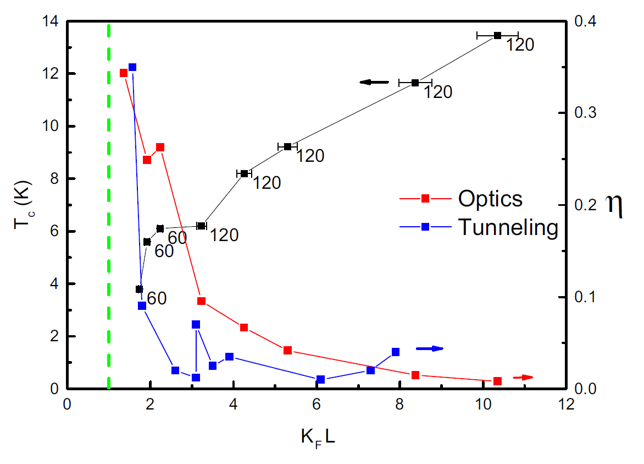
\includegraphics[width=0.49\textwidth]{T_c_disoreder_dependence.png}
	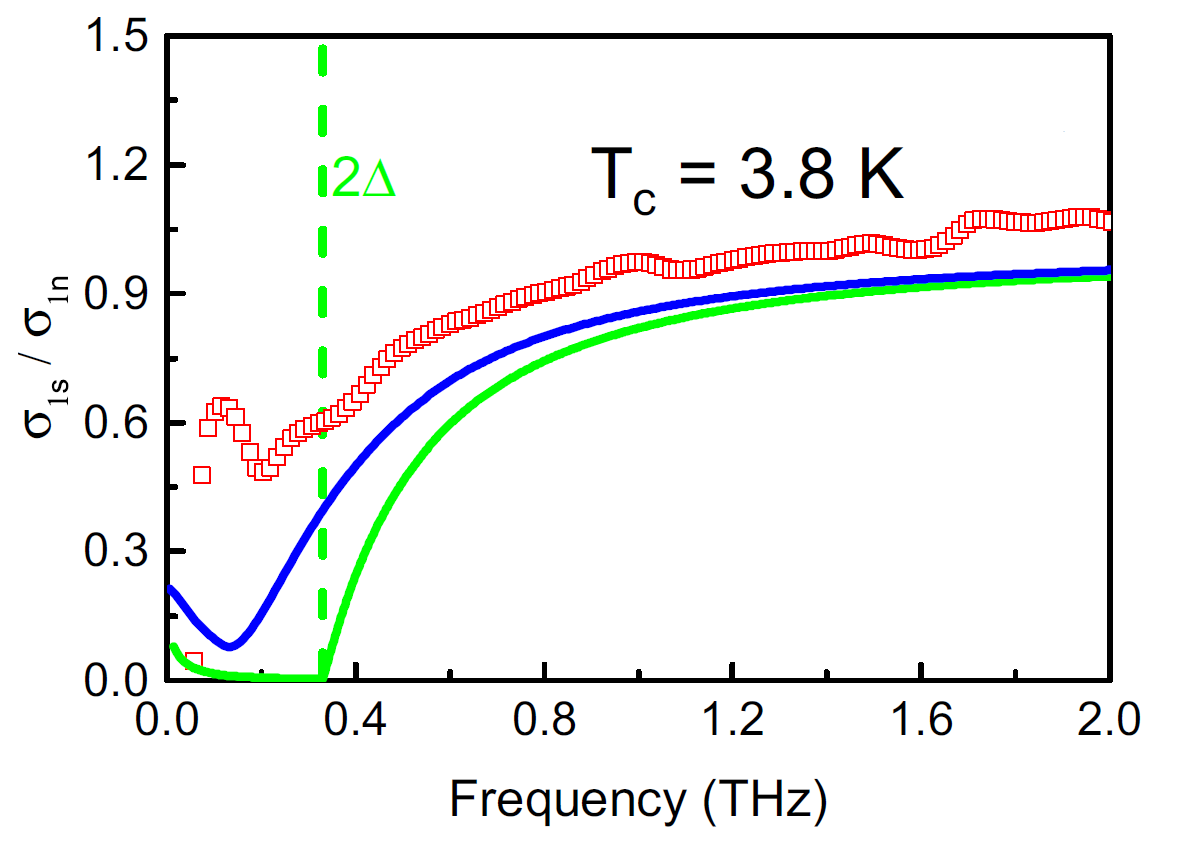
\includegraphics[width=0.4\textwidth]{Real_conductivity_frequency_dependence.png}
	\caption{Демонстрация влияния сильного беспорядка на ключевые свойства сверхпроводимости на примере плёнок NbN. Слева, чёрные символы: зависимость температуры сверхпроводящего перехода от степени загрязнения металла, измеряемой безразмерным параметром $k_F l$, где $k_F$ --- импульс Ферми, а $l$ -- длина свободного пробега. Параметр $k_F l$ определялся по сопротивлению при комнатной температуре. Данные взяты из работы \cite{Cheng_2016}. Справа, красные символы: зависимость действительной части проводимости металла от частоты внешнего излучения. Зелёной линией отмечено положение сверхпроводящей щели, найденное средствами туннельной микроскопии. Данные также взяты из работы \cite{Cheng_2016}.}	
\end{figure}
Выборка из экспериментальных данных, более детально демонстрирующих обсуждаемые эффекты на примере плёнок NbN, приведена на Рис. \ref{fig:Impur_Tc_and_radiation_absorb_data}. Существенно, что обсуждаемые эффекты происходят в макроскопически однородных образцах, где характерные масштабы неоднородностей существенно микроскопические. В частности, беспорядок в плёнках NbN создаётся за счёт вакансий Nb в кристаллической решётке \cite{Cheng_2016}. Схожими свойствами обладают также и ряд других образцов:
\begin{itemize} 
	\item плёнки InO, в которых также наблюдались описываемые явления \cite{Sherman_2015}, и беспорядок в которых имеет стехиометрическую природу, т. е. задаётся аморфной структурой вещества;
	\item плёнки из наногранул Al \cite{Pracht_2016}, в которых микроскопические неоднородности задаются непосредственно структурой из гранул алюминия размерами $\sim 2 nm$, разделённых оксидной плёнкой. В этом случае микроскопичность неоднородностей проявляется в том, что отдельно взятая гранула в силу своих малых размеров не обладает достаточными числом состояний для развития сверхпроводящих эффектов.
\end{itemize}

Эффект изменения температуры перехода $T_c$ в макроскопически однородных загрязнённых образцах уже получил теоретическое описание \cite{Feigelman2010}, и качественно объясняется влиянием эффектов Андерсоновской локализации и преформирования Куперовских пар (несколько подробнее эта эффекты мы разберём далее). Однако этого нельзя сказать о факте наличия низкоэнергетических возбуждений: существует лишь ряд эмпирических теорий, не дающих объяснения природе наблюдаемого явления (см., опять же, \cite{Cheng_2016}, \cite{Sherman_2015}). В данной работе будет произведена попытка разработать количественную микроскопическую модель, описывающую низкоэнергетические возбуждения в грязном сверхпроводнике. Теоретическое описание будет строиться на основе идей, развитых в \cite{Feigelman2010}, а также в значительной степени будет опираться на изложенные в работе \cite{FI_microwave} гипотезы по конкретной реализации упомянутой модели.



\section{Схема организации работы}
Данная работа организована следующим образом:
\begin{itemize}
	\item в \autoref{Theor}, посвящённой непосредственно теоретическому описанию явления низкоэнергетических возбуждений, будет дано подробное описание модельной задачи, предположительно содержащей ключевые эффекты.
	\begin{itemize}
		\item Сначала представлено феноменологическое введение, мотивирующее последующие упрощающие предположения. По итогу будет выписан т. н. псевдоспиновый гамильтониан на $K$-регулярном графе, использующийся далее для описания всей физики <<грязной>> сверхпроводимости.
		\item На его основе с помощью формализма семионного представления Попова-Федотова будут выведены основные уравнения, описывающее сверхпроводящее состояние: уравнение самосогласования и квадратичная часть функционала Гинзбурга-Ландау.
		\item Наконец, построенный формализм позволит поставить задачу, непосредственно описывающую в рамках данной модели низкоэнергетические возбуждения в сверхпроводнике. 
		\item Последним пунктом будут изложены упрощения, позволяющие решить поставленную задачу в терминах локальной плотности состояний некоторого линейного оператора на $K$-регулярном графе. Будут также приведены имеющиеся теоретические предсказания, связанные с этой упрощённой моделью.
	\end{itemize}

	\item в \autoref{Numer} будет подробно изложена теория метода популяционной динамики, предоставляющего способ численного решения поставленной в конце \autoref{Theor} упрощённой задачи.
	\begin{itemize}
		\item Для начала будет приведено введение в теорию, позволяющую установить соответствие между задачами на больших регулярных графах и на древесных графах с постоянным ветвлением.
		\item Далее будет приведён вывод и подробное описание алгоритма популяционной динамики вкупе с проделанными оптимизациями. Будет также установлена связь изучаемых величин с задачей локализации Андерсона с диагональным беспорядком.
		\item Затем будут приведено сравнение алгоритма с уже имеющимся методом исследования схожих задач и разобраны основные особенности поведения данной численной процедуры.
	\end{itemize}

	\item \autoref{Result} представит читателю обзор результатов численного исследования модели, физическую интерпретацию полученных сведений и вывода по дальнейшему изучению.
	\begin{itemize}
		\item Будут представлены подробные результаты, описывающие все важные аспекты статистики локальной плотности состояний упомянутого оператора. 
		\item Для основных характеристик статистики будет приведены имеющиеся численные данные, описывающие зависимости от параметра $K$.
		\item Полученные результаты будут интерпретированы с позиции уже известной теории задачи Андерсона. Будет представлен анализ сделанных ранее качественных и количественных предсказаний касательно этой модели.
		\item Наконец, будет представлена интерпретация полученных результатов в терминах исходной задачи описания низкоэнергетических возбуждений сверхпроводника и намечен план дальнейших исследований.
	\end{itemize}

	\item В финальной \autoref{Concl} приводится краткий обзор проделанной работы и резюмируются сделанные в процессе выводы.
\end{itemize}
%TODO: WRITE a paragraph about notations
% contraction rules, Heaviside function, Pauli matricies, E_F, k_F, l, \tau (Matrsubara imaginary time), \beta = 1/T, 
\chapter{Теоретическое описание} \label{Theor}
\section{Теоретический подход и феноменология неупорядоченных сверхпроводников}
При микроскопическом описании сверхпроводящего состояния традиционным подходом является БКШ-подобные гамильтонианы на основе точных состояний невзаимодействующей системы электронов:
\begin{equation}
\label{eq:BCS_type_Ham}
H_{BCS} = \sum_{j\sigma} \xi_j a_{j\sigma}^\dagger a_{j\sigma} - \frac{\lambda}{\nu_0} \sum_{ijkl} V_{ijkl} a_{i\uparrow}^\dagger a_{j\downarrow}^\dagger a_{k\downarrow} a_{l\uparrow}
\end{equation}
где использованы следующие обозначения:
\begin{itemize}
	\item $i$ --- индекс одночастичного собственного состояния невзаимодействующей системы c энергией $\xi_j$,
	\item $a_{j\sigma}^\dagger, a_{j\sigma}$ --- фермионные операторы рождения уничтожения соответствующего состояния,  $\sigma$ --- спиновый индекс,
	\item $\nu_0$ --- плотность одночастичных состояний системы,
	\item константа $\lambda$ характеризует притягивающее Куперовское взаимодействие, обрезаемое на некотором энергетическом масштабе $\varepsilon_0$; предполагается, что  зависимостью притягивающего взаимодействия от импульса можно пренебречь, т. е. считать его точечным;
	\item $V_{ijkl}$ содержит в себе информацию о перекрытии уровней и амплитуде туннелирования между этими состояниями
\end{itemize}

Для возможности теоретического рассмотрения задачи необходимо сделать дальнейшие упрощения, касающиеся деталей устройства одночастичных состояний и их перекрытий. К сожалению, до сих пор не построено последовательной теории, позволяющей эти упрощения обосновать и выяснить критерии их применимости, поэтому изложенные ниже предположения в значительной степени будут обоснованы исключительно качественно за счёт феноменологии и экспериментальных данных. Подробное обсуждение модели \eqref{eq:BCS_type_Ham} и постулируемых далее приближений можно также найти в \cite{Feigelman2010}.


\subsection{Преформирование электронных пар}
%ЗДЕСЬ ЕЩЕ ВПИСАТЬ ССЫЛКУ НА SACEPE, FEIGELMAN 2011 NATURE, есть в [7]
%Решил не включать, потому что ссылка на эту работу есть в \cite{Dubouchet_et_al_2018}, и изложено там +- тоже самое. Плюс, МВ кидал ссылку и на \cite{Dubouchet_et_al_2018}, так что все ок.
Для упрощения модели требуется уточнить структуру самих матричных элементов $V_{ijkl}$, для чего мы привлечём экспериментально наблюдаемое явление наличия т. н. псевдощели. Суть данной концепции заключается в видимом присутствии парных электронных образований даже при отсутствии коллективных сверхпроводящих эффектов. Это явление экспериментально обнаруживается по различию спектров одночастичных и двухчастичных возбуждений, выявленных методами туннельной андреевской спектроскопии \cite{Dubouchet_et_al_2018}, а также по данным измерения проводимости в некоторых изоляторах вблизи сверхпроводящего перехода, демонстрирующих термоактивационное поведение сопротивления \cite{Shahar_Ovadyahu_1992}. Важные для рассматриваемой нами модели феноменологические аспекты и выводы из экспериментальных данных для этого явления таковы:
\begin{itemize}
	\item В широком диапазоне температур, включающем в себя температуру сверхпроводящего перехода $T_c$, электроны в системе представлены связанными парами с суммарным нулевым спином, причём каждая пара занимает некоторое одночастичное состояние.
	\begin{itemize}
		\item Причина притяжения, обуславливающего такое поведение, является предметом обсуждения. Хорошим кандидатом выглядит непосредственно само Куперовское притяжение, поскольку локализационный объём одного состояния достаточно большой для развития этого эффекта. Это контролируется параметром $\nu_0 V_{loc} \varepsilon_0 \gg 1$, где $\varepsilon_0$ -- энергетическая обрезка Куперовского притяжения в гамильтониане \eqref{eq:BCS_type_Ham}.
	\end{itemize}
	
	\item Энергия разрыва этих пар $\Delta_P$ значительно превышает все сверхпроводящие масштабы энергий, вроде амплитуды параметра порядка $\Delta$ и температур перехода $T_c$. 
	\begin{itemize}
		\item По существу это означает, что электроны по системе перемещаются в основном парами, что также означает ярко выраженные эффекты чётности. Поскольку нашей исходной задачей является описание низкоэнергетической физики системы, то логичным предположением будет исключение одночастичных состояний из рассмотрения, и учёт лишь динамики состояний электронных пар.
	\end{itemize}
\end{itemize} 
Исходя из этих фактов, нашу модель можно дополнить следующими приближениями, упрощающими структуру члена со взаимодействием в гамильтониане \eqref{eq:BCS_type_Ham}.
\begin{itemize}
	\item В динамике системы участвуют только состояния с числами заполнения $n_i = 0\text{ или }2$, поскольку состояние с $n_i = 1$ отделено большой щелью.
	\item Соответственно, мы можем допустить, что основную роль играют процессы прыжков электронных пар между состояниями, так что из всех матричных элементов в гамильтониане \eqref{eq:BCS_type_Ham} мы оставим только полудиагональные вида $V_{iijj}$.
	\item Диагональные матричные элементы $V_{iiii}$, описывающие самовзаимодействие, мы также считаем нулевыми (считаем, что их эффект сводится к перенормировке энергии узла). 
\end{itemize}


\subsection{Одночастичная локализация точных состояний}
Поскольку образцы, в которых наблюдается исследуемый нами феномен наличия низкоэнергетических возбуждений, при температурах выше температуры перехода демонстрируют свойства изолятора, то это свидетельствует о проявлении в этих образцах эффектов одночастичной локализации Андерсона. Феноменология этого эффекта уже хорошо изучена, обзор основных результатов можно найти, например, в \cite{Lee_Ramakrishnan_1985}. Качественно важные для нас свойства Андерсоновской локализации можно резюмировать следующим образом: 
\begin{itemize}
	\item при достижении силы беспорядка (например, концентрации примесей) некоторого критического значения одночастичные волновые функции электронов перестают быть делокализованными по всему образцу (как это было бы в случае Блоховских волновых функций), и обретают некоторый конечный локализационный объём, за пределами которого их амплитуда экспоненциально мала.
	\item В широком диапазоне значения силы беспорядка (в т. ч. ниже критического) волновые функции характеризуются так называемой фрактальной структурой, которая количественно описывается степенной зависимостью от занимаемого объёма различных моментов амплитуды волновой функции с нетривиальным показателем:
	$$
	P^{(q)} := \left\langle |\psi_i(r)|^q \right\rangle \sim V_{loc}^{d_q}
	$$
	где усреднение ведётся по координате $r$, пробегающей весь объём образца. Качественно это поведение означает, что волновая функция сложным (самопободобным) образом хорошо выражена лишь в части занимаемого ей объёма.
	\item Перекрытия состояний также приобретают фрактальную статистику, характеризуемую степенной зависимостью перекрытий от разности энергий $\xi_i$ соответствующих состояний:
	$$
	C_{ij} := \left\langle \psi_i(r) \psi_j^{*}(r) \right\rangle \sim \left| \xi_i - \xi_j \right|^{d_{overlap}}
	$$
\end{itemize}
Подробное обсуждение этих эффектов также имеется в \cite{Feigelman2010}. К сожалению, строгий учёт этих эффектов представляется весьма трудоёмкой процедурой, не позволяющей до сих пор выделить ключевые феноменологические аспекты. Поэтому предлагается сделать качественные упрощения, которые сохраняют предположительно существенную феноменологию:
\begin{itemize}
	\item будем считать, что система находится неглубоко в фазе изолятора, т. е. в таких условиях, когда локализационный объём $V_{loc}$ уже не является макроскопической величиной порядка размеров  реальных систем, однако он все ещё содержит в себе большое количество одночастичных состояний, позволяя развиваться механизмам Куперовского притяжения, что контролируется параметром $\nu V_{loc} \epsilon_0 \gg 1$.
	\item Абсолютная величина перекрытия состояний воспроизводится довольно грубо: в рамках нашей модели перекрытие или имеется с некоторой постоянной амплитудой, не зависящей от выбранной пары узлов, или не имеется вовсе. Мы заменяем, вообще говоря, нетривиальное и коррелированное между различными парами узлов распределение совокупности матричных элементов $V_{iijj}$ в гамильтониане \eqref{eq:BCS_type_Ham} на его сильно упрощённый вариант, делящий все пары состояний на связанные и несвязанные. При этом характерным значением, определяющее это разделение, естественным образом будет являться энергия Куперовского притяжения.
	\item Учёт фрактальной структуры волновых функции внутри локализационного объёма мы также проведём очень качественно: будем считать, что у каждого узла имеется некоторое большое \textit{постоянное} число $K + 1 \gg 1$ ненулевых перекрытий \textit{случайно выбранным множеством состояний}. Разумеется, последнее предположение нарушает локальные свойства модели, потенциально разрешая перекрытия между двумя очень далёкими в реальном пространстве состояниями, однако здесь мы предполагаем, что ни флуктуации реального числа перекрытий от узла к узлу, ни  прыжки на большие расстояния не определяют реальную физику происходящего процесса.
	\item Плотность состояний невзаимодействующей системы мы будем моделировать простым распределением ширины $W \sim E_F$ с ненулевой плотностью состояний в центре зоны. Данное приближение обосновано постольку, поскольку по сравнению с характерным масштабом изменения плотности состояний (этот масштаб как раз $\sim E_F$) все прочие энергетические величины, не превышающие обменной энергии Куперовского взаимодействия $\varepsilon_0 \ll E_F$ пренебрежимо малы, так что изменением плотности состояний можно не учитывать. 
\end{itemize}
Подчеркнём, что приближения, моделирующие статистику перекрытий состояний, являются очень качественными, так как любые уточнение в сторону более точной картины на данный момент не позволяют добиться построения решаемой модели. Мы надеемся, что основная физика явления доставляется лишь тем фактом, что каждый узел связан с большим числом прочих узлов с близкими между собой значениями туннельных амплитуд, каждая из которых порядка энергии Куперовского взаимодействия $\varepsilon_0$, а редко встречающиеся флуктуации (их редкость, вообще говоря, тоже весьма условна) не являются определяющими.


\subsection{Итоговая модель}
Перед окончательной формулировкой модели дадим ещё один небольшой комментарий: гамильтониан \eqref{eq:BCS_type_Ham} не учитывает Кулоновское взаимодействие электронов. Количественная степень обоснованности этого пренебрежения до сих пор понята очень плохо, и основные аргументы в пользу такого приближения апеллируют к экспериментальным фактам, основным из которых является независимость поведения псевдощели и истинного параметра порядка при сверхпроводящем переходе, в то время как Кулоновское взаимодействие должно подавлять оба явления одинаковым образом. С имеющимися точками зрения а также основными аргументами в пользу пренебрежения Кулоновским взаимодействия можно ознакомиться в \cite{Feigelman2010}.

Резюмируя все рассуждения выше, можем перечислить итоговые предположения рассматриваемой в этой работе модели:
\begin{enumerate}
	\item Электроны во всём существенном для задачи диапазоне температур образуют пары с нулевым суммарным спином, каждая из которых занимает некоторое одночастичное состояние и физически локализована в конечном объёме.
	\item Разрывом этих пар в задаче можно пренебречь.
	\item Кулоновское взаимодействие также можно не учитывать.
	\item Перемещения электронов описываются прыжками пар между состояниями.
	\item Каждое состояние имеет \textit{постоянное} перекрытие с большим \textit{постоянным} числом соседей $Z = K + 1 \gg 1$.
	\item Соседствующие между собой узлы выбираются \textit{случайным} образом, без какой-либо регулярной структуры.
	\item Энергии парных состояний можно считать некоррелированными случайными величинами, подчиняющимися некоторому распределению конечной большой ширины $W \sim E_F$.
	\item В дальнейшем мы будем интересоваться низкотемпературным поведением модели
\end{enumerate}
Данные утверждения позволяют записать практически окончательную форму гамильтониана:
\begin{equation}
\label{eq:Ham_physical}
H_{model} = \sum_{j\sigma} \xi_j a_{j\sigma}^\dagger a_{j\sigma} - \frac{g}{K} \sum_{(ij)} a_{i\uparrow}^\dagger a_{i\downarrow}^\dagger a_{j\downarrow} a_{j\uparrow}
\end{equation}
где
\begin{itemize}
	\item $i,j$ --- узлы некоторого случайного $K$-регулярного графа (т. е. такого графа, у которого число соседей каждой вершины постоянно и равно $Z = K + 1$) с термодинамическим большим числом узлов $M$, а сумма в члене со взаимодействием происходит по рёбрам этого графа;
	\item $\xi_i$ --- энергии соответствующих состояний, представляемые \textit{независимыми одинаково распределенными случайными величинами} с плотностью распределения $P(\xi) = \frac{1}{2 W}\theta(W - |\xi|)$; заметим, что величина $W$ также определяет плотность состояний в невзаимодействующей системе: $\nu_0 \cdot 2 W = 1$;
	\item Сила взаимодействия определяется константой $g$, вбирающей в себя характеристики силы Куперовского спаривания и перекрытия состояний. Лишний множитель $1/K$ во взаимодействии призван корректно воспроизводить предел чистого сверхпроводника (по существу, он также является частью величины перекрытия состояний).
\end{itemize} 

Далее являются удобными следующие упрощения:
\begin{itemize}
	\item переход на новые энергетические единицы $W$, что избавляет от лишней константы, и потому можно положить
	$$
	P(\xi) = \frac{1}{2}\theta(1 - |\xi|)
	$$
	\item введение так называемых псевдоспиновых операторов, осуществляющих отображение на задачу системы взаимодействующих спинов $s = 1/2$ на случайном графе:
	\begin{align}
	\label{pseudospin_op}
		2s^z_j & = \sum_\sigma a_{j\sigma}^\dagger a_{j\sigma} - 1 &
		s^+_j & = a_{j\downarrow}^\dagger a_{j\uparrow}^\dagger &
		s^-_j & = a_{j\downarrow} a_{j\uparrow}
	\end{align}
\end{itemize}
В результате этих упрощений, окончательное выражение имеет хорошо известный вид т. н. псевдоспинового гамильтониана \cite{Ma_Lee_1985}:
\begin{equation}
\label{eq:Ham_final}
H_{PS} = \sum_{j} 2 \xi_j s_j^z - \frac{g}{K} \sum_{(ij)} (s_i^+ s_j^- + h.c) \equiv \sum_{j} 2 \xi_j s_j^z - \frac{2g}{K} \sum_{(ij)} (s_i^x s_j^x + s_i^y s_j^y)
\end{equation}
Таким образом, поставлена задача об изучении устройства основного состояний и элементарных возбуждений гамильтониана \eqref{eq:Ham_final}.

В заключение сделаем важное физическое замечание: гамильтониан \eqref{eq:Ham_final} \textit{полностью исключает из задачи} детали устройства одночастичных состояний в реальном пространстве. Поэтому полученные в рамках этой модели ответы, должны интерпретироваться, строго говоря, только в сочетании со знанием статистики взаимного расположения одночастичных состояний в реальном пространстве.



\section{Основные уравнения теории сверхпроводимости}
\subsection{Представление семионов Попова-Федотова}
Отправной точкой построения функционального интеграла для псевдоспинового гамильтониана \eqref{eq:Ham_final} будет являться хорошо известное \textit{семионное представление Попова-Федотова} \cite{Popov_Fedotov}. 
%Более полный формализм, обобщающий данное представление, а также дающий полезные математические сведения касательно этого метода, можно найти в \autoref{App_Semion}. 
Эта техника получила обобщение на случай произвольного спина $s$ (с некоторыми оговорками), с примером её применения в общем виде можно ознакомиться, например, в \cite{Veits_etal_1994}. В этой работе же будут даны только необходимые для дальнейшего вывода сведения.

\subsubsection{Определения}
Рассмотрим стандартное представление спиновой алгебры $\mathfrak{su}_2$ со спином $s = 1/2$.
\begin{itemize}
	\item Спиновые операторы будем обозначать маленькими буквами: $s^x, s^y, s^z$. Эти операторы весьма очевидным образом связаны с матрицами Паули. Элементы алгебры мы будем далее отождествлять с их каноничным представлением.
	\item Пространство состояний, на котором строится представление, обозначим $V^S$. В качестве базиса возьмём собственные вектора оператора $z$-проекции спина: $\left\{ \left|s, m\right>: m\in[-s,s] \right\}$. Полная размерность пространства, очевидно, равна $\dim V^S = 2s+1$.
	\item Коммутационные соотношения в алгебре стандартны: $ \left[ s^i, s^j \right]_{-} = i \epsilon^{ijk} s^k $.
\end{itemize}
Введём также алгебру $\mathfrak{f}$ операторов рождения и уничтожения фермионов, которые могут находиться в одном из $2s+1 = 2$ состояний.
\begin{itemize}
	\item Операторы рождения и уничтожения фермиона в соответствующем состоянии будем нумеровать нижним индексом:	$\left\{ c_k, c_k^\dagger: k\in[-s,s] \right\} $
	\item Полное Фоковское пространство состояний, обозначим как $V^F$. Базисными векторами в этом пространстве будут собственные вектора оператора числа частиц в конкретном состоянии: $\left\{ \left| n_1,...n_{2s+1} \right>: n_k \in \{0, 1\} \right\}$. Полная размерность есть $\dim V^F = 2^{2s+1} = 4$
	\item Фермионные операторы обладают стандартными правилами коммутации с обычными антикоммутационными соотношениями	$\left\{ c_i, c^\dagger_j \right\}_{+} = \delta_{ij} $, 
	где $\{a,b\}_{+} =: ab + ba$ --- антикоммутатор.
	\item Здесь нам также понадобятся инвариантные подпространства оператора полного числа частиц
	$$N = \sum_{k = -s}^{s} c^\dagger_k c_k \equiv \sum_{k = -s}^{s} N_k$$.
	Подпространство с полным число частиц $n$ мы будем обозначать за $V^F_n$, а базисные вектора это подпространства, являющиеся подмножеством полного набора базисных векторов, мы переобозначим так, что будем указывать там множество занятых состояний: 
	$$\left\{ \left| B \right>: B \subset \overline{\{1,n\}}, |B| = n, N_k \left| B \right> = \begin{cases}
	1, & k\in B\\
	0, & k\notin B
	\end{cases}  \right\}$$
	Очевидно, размерность соответствующего подпространства $\dim V^F_n = C_{2s+1}^n$. Конкретно в случае $s = 1/2$ имеем три подпространства $\dim V^F_0 = 1$, $\dim V^F_1 = 2$,  $\dim V^F_2 = 1$.
\end{itemize} 

\subsubsection{Запись представления}
Представление определяется следующим оразом: каждому оператору $a \in \mathfrak{su}_2$ сопоставляется оператор $A \in \mathfrak{f}$ по формуле
\begin{equation}
\label{eq:semion_repr}
A = \sum_{m, n = - s}^s c^\dagger_m \left\langle m \left| a \right| n \right\rangle c_n
\end{equation}
Для этого представления выполнены следующие важные свойства:
\begin{itemize}
	\item на подпространстве $V^F_1$ ферминонного пространства состояний осуществляется мономорфизм представления спиновой алгебры в представление фермионной Иными словами, на $V^F_1$ матричные элементы соответствующих операторов одинаковые:
	$$ \left\langle {m} \left| A \right| {n} \right\rangle =  \left\langle m \left| a \right| n \right\rangle $$
	Это очевидно из построения.
	
	\item Для $s = 1/2$ верно дополнительно следующее: на ортогональном дополнении к физическому пространству состояний $\left( V^F_1 \right)^\perp$ все операторы вида \eqref{eq:semion_repr} тождественно равны нулю:
	$$ A \left| 1, 1\right\rangle = A \left| 0, 0 \right\rangle = 0$$
	Это является следствием того факта, что представление алгебры $\mathfrak{su}_2$ --- бесследовое: $ \Tr s^i = 0 $.
	
	\item Наконец, если теперь рассмотреть тензорное произведение алгебр, соответствующей, скажем, локальным операторам на узлах графа, то очевидным является распространение вышеуказанных утверждений и на этот случай. Иными словами, это представление без изменений применимо и для системы спинов.
\end{itemize}

\subsubsection{Воспроизведение статистических свойств}
Полученное представление даёт возможность взаимно однозначно отобразить задачу исследования равновесной термодинамики псевдоспинового гамильтониана \eqref{eq:Ham_final} на оную для взаимодействующей системы фермионов с тем же парным взаимодействием. Формально это выглядит следующим образом:
\begin{enumerate}
	\item Пусть имеется произвольный спиновый гамильтониан $H^S$, действующий на пространстве состояний некоторого множества спинов $s = 1/2$. Сопоставим ему фермионный гамильтониан $H^F$, получаемый из $H^S$ формальной заменой всех спиновых операторов на фермионные по формуле \eqref{eq:semion_repr} (ну или же можно применить формулу \eqref{eq:semion_repr} сразу ко всему гамильтониану $H^S$, рассматривая при этом тензорное произведение представлений алгебры на узле). Тогда статистические суммы для спинового гамильтониана отличается лишь фазовым множителем от статистической суммы фермионного гамильтониан с мнимым хим. потенциалом $\mu_0 = \frac{i \pi}{2 \beta}$:
	$$
	Z^S(\beta) := \Tr \exp \left\{-\beta H^S\right\} = i^M \Tr \exp \left\{ -\beta H^F + \beta \mu_0 N\right\} =: i^M \mathcal{Z}^F(\beta, \mu_0)
	$$
	где $M$ --- полное число узлов в системе, а $\beta \equiv \frac{1}{T}$ --- обратная температуры. Обратим ещё раз внимание, что в левой части равенства след берётся по спиновому пространству состояний, а в правом --- по полному Фоковскому пространству фермионов.
	\item Немедленным следствием предыдущего утверждения является важное для практического применение утверждение о совпадении средних: среднее \textit{любого} оператора $x$ на системе спинов (будь то одного оператора спина, или любого их произведения) совпадает со средним для оператора $X$, получаемого из $x$ формальной заменой спиновых операторов по формуле \eqref{eq:semion_repr}, с таким же образом полученным фермионным гамильтонианом с мнимым хим. потенциалом:
	\begin{equation}
		\label{eq:semion_mean_correspondence}
		\left\langle x \right\rangle := \frac{\Tr\left[ x \exp\left\{-\beta H^S\right \} \right]}{Z^S} =  \frac{\Tr\left[ X \exp\left\{-\beta H^F + \beta \mu_0 N\right\} \right]}{\mathcal{Z}^F} =: \left\langle X \right\rangle
	\end{equation}
	Это легко увидеть, рассмотрев производящую функцию средних, которая также является стат. суммой некоторого гамильтониана.
\end{enumerate}

\subsubsection{Формулировка исходной задачи в терминах семионов}
Резюмируем полученный результат конкретно для интересующего нас случая: вместо исходной системы \eqref{eq:Ham_final} можно рассматривать равновесную термодинамику следующего фермионного гамильтониана
\begin{equation}
	\label{eq:Ham_semion}
	H_{PS}^F = \underset{H^F_0}{\underbrace{ \sum_{j} \xi_j \sigma^z_{\alpha \beta} c^\dagger_{j\alpha} c_{j\beta} }} \underset{H^F_{int}}{\underbrace{ - \frac{2g}{K} \sum_{(ij)} \frac{1}{4} \left( \sigma^x_{\alpha \beta} \sigma^x_{\rho \eta} + \sigma^y_{\alpha \beta} \sigma^y_{\rho \eta} \right) c^\dagger_{i\alpha} c_{i\beta} c^\dagger_{j\rho} c_{j\eta} }}
\end{equation}

Пояснения:
\begin{itemize}
	\item $c^\dagger_{j\alpha},  c_{j\alpha}$ --- операторы рождения и уничтожения фермиона на узле $j$ в состоянии $\alpha$. Таким образом, подразумевается, что на каждом узле имеется $2s+1 = 2$ внутренних состояния, в которых может находиться фермион. 
	
	\item $\sigma^i_{\alpha\beta}$ --- матрицы Паули, воспроизводящие матричные элементы соответствующих спиновых операторов в каноничном базисе собственных состояний $z$-проекции спина. Во всей записи по повторяющимся греческим индексам подразумевается суммирование. Таким образом, мы получили систему фермионов с \textit{парным локальным взаимодействием}.
	
	\item В формуле также явно отражён факт разделения на голый гамильтониан фермионов $H^F_0$ и член взаимодействия $H^F_{int}$.
	
	\item Более общо, любому оператору исходной задачи с псевдоспиновым гамильтонианом \eqref{eq:Ham_final} ставится в соответствие его семионное представление посредством замены каждого спинового оператора по правилу \eqref{eq:semion_repr}.
	
	\item При этом в статистической сумме хим. потенциал принимает чисто мнимое значение $\mu_0 = \frac{i \pi}{2 \beta}$.
\end{itemize}


\subsection{Функциональный интеграл для псевдоспинового гамильтониана}
Благодаря построенному семионному представлению, к задаче теперь можно применять методы функционального интегрирования. Функциональный интеграл по фермионным переменным для многочастичной задачи строится стандартным образом \cite{Altland_Simons}.
\begin{enumerate}
	\item Введём набор Грассмановых антикоммутирующих переменных, соответствующих операторам рождения и уничтожения исходной задачи
	\begin{equation}
		\label{eq:Grassman_field_def}
		\begin{split}
			& \left\{ \overline{\psi}_{i\alpha}, \psi_{i\alpha}: \alpha \in \overline{[-s,s]}, i \in \overline{1,M}\right\} \\
			& \forall i,j,\alpha,\beta \hookrightarrow
			\left\{  \psi_{i\alpha}, \psi_{j\beta} \right\} _{+} = 
			\left\{  \overline{\psi}_{i\alpha}, \psi_{j\beta}  \right\} _{+} = 
			\left\{  \overline{\psi}_{i\alpha}, \overline{ \psi_{j\beta} } \right\} _{+} = 0
		\end{split}
	\end{equation}
	
	\item Определим функцию Гамильтона от этих переменных, которая получается формальной подстановкой $c^\dagger_{i\alpha} \mapsto \overline{\psi}_{i\alpha}, c_{i\alpha} \mapsto \psi_{i\alpha}$ в \textit{нормально упорядоченный} фермионный гамильтониан \eqref{eq:Ham_semion}. К счастью, благодаря тому, что в рассматриваемой системе узел не взаимодействует непосредственно сам с собой (во взаимодействии нет слагаемых с $i = j$), за счёт нормального упорядочения новых членов не появится, так что упомянутая функция будет иметь вид
	\begin{equation}
		\label{eq:Ham_grassman}
		H^G\left( \overline{\psi}, \psi \right) = \underset{H_0^G}{\underbrace{ \sum_{j} \xi_j \tau^z_{\alpha \beta} \overline{\psi}_{j\alpha} \psi_{j\beta} }} \underset{H_{int}^G}{\underbrace{ - \frac{2g}{K} \sum_{(ij)} \frac{1}{4}(\sigma^x_{\alpha \beta} \sigma^x_{\rho \eta} + \sigma^y_{\alpha \beta} \sigma^y_{\rho \eta}) \overline{\psi}_{i\alpha} \psi_{i\beta} \overline{\psi}_{j\rho} \psi_{j\eta} }}
	\end{equation}
	где снова явно отражено разделение членов, аналогичное \eqref{eq:Ham_semion}.
	Требуется также ввести функцию числа частиц
	\begin{equation}
		\label{eq:N_grassman}
		N^{G}\left( \overline{\psi}, \psi \right) = \sum_{j} \overline{\psi}_{j\alpha} \psi_{j\alpha}
	\end{equation}
	
	\item Для определения функционального интеграла отрезок $[0,\beta]$ мнимого Мацубаровского времени разбивается на $N_0 \rightarrow \infty$ одинаковых кусков, и поля $\overline{\psi}_{i\alpha}, \psi_{i\alpha}$ имеют на участке $\left[ (n-1)\frac{\beta}{N_0}, n\frac{\beta}{N_0} \right]$ значение соответственно $\overline{\psi}_{i\alpha}[n], \psi_{i\alpha}[n]$. Грассмановы поля починяются условию антипериодичности 
	\begin{equation}
		\label{eq:Psi_boundary_cond}
		\psi_{i\alpha}(\tau=0) \equiv \psi_{i\alpha}[n = 0] = - \psi_{i\alpha}[n = N_0] \equiv -\psi_{i\alpha}(\tau=\beta),
	\end{equation}
	и аналогично для сопряжённого поля $\overline{\psi}_{i\alpha}$.
	
	\item Вводится мера функционального интегрирования
	$$
	D\left(\overline{\psi},\psi\right) = \prod_{n = 0}^{N_0 - 1} \prod_{i = 1}^{M} \prod_{\alpha = 1}^{2} d\overline{\psi}_{i\alpha}[n] d\psi_{i\alpha}[n]
	$$
	и действие (вес функционального интегрирования)
	\begin{equation}
		\label{eq:Action_discretized}
		\begin{split}
			\mathcal{A} \left[\overline{\psi}, \psi\right] & = \frac{\beta}{N_0} \sum_{k = 0}^{N_0 - 1}  \left[ \frac{\overline{\psi}_{i\alpha}[n] - \overline{\psi}_{i\alpha}[n + 1]}{\beta/N_0} \psi_{i\alpha}[n] - \right. \\ 
			& \left. -  H^{G}\left(\overline{\psi}[n+1],\psi[n] \right) + \mu_0 N^{G}\left(\overline{\psi}[n+1],\psi[n] \right) \right]
		\end{split}
	\end{equation}
	
	\item Наконец, статистическая сумма посредством использования аппарата когерентных состояний \cite{Altland_Simons} выражается через функциональный интеграл:
	\begin{equation}
		\label{eq:Part_sum_discretized}
		\mathcal{Z}^{F} = \lim_{N_0 \rightarrow \infty} \int \limits_{\mathbb{R}} D\left(\overline{\psi}, \psi\right) \exp\left\{ - \mathcal{A} \left[\overline{\psi}, \psi\right] \right\}
	\end{equation}
	Это выражение также принято записывать в виде непрерывного перехода:
	\begin{align}
		\label{eq:Part_sum_func_int}
		\mathcal{Z}^{F} & = \int \limits_{ \begin{array}{cc}
			\psi(0) = - \psi(\beta)\\
			\overline{\psi}(0) = - \overline{\psi}(\beta)
			\end{array} } 
		D\left(\overline{\psi},\psi\right) \exp\left\{ -\mathcal{A} \left[\overline{\psi}, \psi\right] \right\} \\
		\label{eq:Action}
		\mathcal{A} \left[\overline{\psi}, \psi\right] & = \int\limits_{0}^{\beta} d\tau \left[\sum_{i} \frac{\partial \overline{\psi}_{i\alpha} }{ \partial \tau } \psi_{i\alpha} - H^{G}\left(\overline{\psi},\psi\right) + \mu_0 N^{G}\left(\overline{\psi},\psi\right) \right]
	\end{align}
	В такой записи надо иметь в виду, что поля $\overline{ \psi}$ берутся инфинитезимально позже полей $\psi$. Это будет важно при вычислений средних.
	
	\item Для полного описания равновесной термодинамики исходной системы \eqref{eq:Ham_final} необходимо уметь считать Мацубаровские разновременные корреляторы вида
	\begin{equation}
		\label{eq:Spin_correl_def}
		C^{j_1 j_2 ... j_n}_{i_1 i_2 ... i_n} \left( \tau_1, \tau_2, ... \tau_n \right) := \left\langle T_\tau\left\{ s^{j_1}_{i_1}(\tau_1) s^{j_2}_{i_2}(\tau_2) ... s^{j_n}_{i_n}(\tau_n) \right\} \right\rangle
	\end{equation}
	где использовано обозначение
	$$
	s^j_{i}(\tau) = \exp \left\{ \tau H_{PS} \right\} s^j_i \left\{ - \tau H_{PS} \right\}
	$$
	оператора $j$-ой проекции спина на $i$-ом узле в представлении Мацубары, а $T_\tau$ -- оператор упорядочения по времени, расставляющий операторы в порядке убывания времени $\tau$ слева направо.
	Используя соответствие \eqref{eq:semion_mean_correspondence} и аппарат когерентных состояний устанавливается формула (пределы функционального интегрирования и аргументы действия $\mathcal{A}$ опущены для краткости):
	\begin{align}
		\label{eq:Correlator_funct_int_expression}
		C^{j_1 j_2 ... j_n}_{i_1 i_2 ... i_n} & = \frac{1}{\mathcal{Z}^F} \int D\left(\overline{\psi},\psi\right) \left\{ S^{j_1}_{i_1}(\tau_1) S^{j_2}_{i_2}(\tau_2) ... S^{j_n}_{i_n}(\tau_n) \right\} \exp\left\{ -\mathcal{A} \right\} \\
		\label{eq:Operator_grassman_expression}
		S^j_i(\tau) & = \frac{1}{2} \overline{\psi}_{i\alpha}(\tau + 0) \sigma^j_{\alpha\beta} \psi_{i\beta}(\tau)
	\end{align}
	Снова обращаем внимание, что в последнем определении явно выделено, что поле $\overline{\psi}$ берётся инфинитезимально позже поля $\psi$.
	
	\item В заключение заметим, что путём формального разложения экспоненты в \eqref{eq:Part_sum_func_int} по степеням члена взаимодействия и последующего использования теоремы Вика можно получить правила стандартной Мацубаровской диаграммной техники, которые будут описаны ниже.
	
\end{enumerate}

\subsection{Введение поля параметра порядка}
Чтобы корректно отразить эффекты качественной перестройки основного состояния, происходящие при сверхпроводящем переходе, в задачу следует ввести поле параметра порядка. Эта процедура производится обычном образом \cite{Altland_Simons}, который далее будет кратко изложен. Общий физический смысл введения параметра состоит в построении эффективной длинноволновой теории поля  для исходной задачи.

\subsubsection{Введение бозонного поля параметра порядка}
Проделаем преобразование Хаббарда-Стратановича над функциональным интегралом для члена со взаимодействием. Для этого рассмотрим на каждом узле $i$ векторное поле $\Delta^k_i$ с двумя компонентами $k = x,y$. Заметим, что у бозонного поля $\Delta$ граничные условия по мнимому времени соответствуют периодическим, в отличие от фермионного случая \eqref{eq:Psi_boundary_cond}, что явно отражено в пределах интегрирования нового функционального интеграла.
\begin{align}
	\label{eq:Hubbard_Stratanovich_transrom}
	& \exp\left\{ -\mathcal{A}\left[ \overline{\psi}, \psi \right] \right\}  = \int\limits_{\Delta^k_i(0) = \Delta^k_i(\beta)} D(\Delta) \exp\left\{ -\mathcal{A}_{0}\left[ \overline{\psi}, \psi, \Delta \right] -\mathcal{A}_{int}\left[ \overline{\psi}, \psi, \Delta \right] \right\} \\
	\label{eq:Total_quadratic_action}
	& \mathcal{A}_{0} = \int\limits_{0}^{\beta} d\tau \left[ \frac{1}{2} \left(\frac{K}{2g}\right) 4\sum_{ij} \sum_k \Delta^k_i J^{-1}_{ij} \Delta^k_j + \sum_{i} \frac{\partial \overline{\psi}_{i\alpha} }{ \partial \tau } \psi_{i\alpha} - H^{G}_0 + \mu_0 N^{G} \right] \\	
	\label{eq:Boson_fermion_interaction_action}
	& \mathcal{A}_{int} = -\int\limits_{0}^{\beta} d\tau \left[ - \sum_{i} \sum_k \Delta^k_i \overline{\psi}_{i\alpha} \sigma^k_{\alpha\beta} \psi_{i\beta} \right] 
\end{align}
где введено обозначение $J_{ij}^{-1}$ обращения матрицы смежности графа. В общем случае эта матрица может быть необратимой, что, однако, исправляется посредством введения постоянной сдвижки, к которой финальные ответы будут нечувствительны, так что далее будем считать эту матрицу всегда обратимой. Поскольку мера матриц $J_{ij}$ с наличием строго нулевого собственного числа равна 0 (это можно показать, например, используя Лемму Сарда $\det J$ как функции своих аргументов), то данная процедура регуляризации не испортит исследуемый ансамбль.
%TODO: WRITE verify the statement above. Lyubshin?

Таким образом, осуществлён переход к системе из фермионного и бозонного полей, взаимодействующих контактным (лишь на совпадающих узлах) потенциалом. Физический смысл введённой величины состоит в описании аномального среднего, возникающего в сверхпроводнике, и характеризующего нарушение $U(1)$-симметрии.

\subsubsection{Избавление от фермионных степеней свободы}
Следующим шагом следует перейти к описанию динамики чисто бозонных полей. Для этого следует явно взять функциональный интеграл по фермионным степеням свободы, что возможно благодаря тому, что полное действие $\mathcal{A}_0 + \mathcal{A}_{int}$ является квадратичным по Грассмановым полям $\psi$. Взятие Грассманового интеграла тогда приводит к следующему результату:
\begin{align}
	\label{eq:Part_sum_thorugh_boson_functional_integral}
	& \mathcal{Z}^F = \int D(\Delta) \exp\left\{ -\int\limits_{0}^{\beta} d\tau \left[ 2 \left(\frac{K}{2g}\right) \sum_{ij} \sum_k \Delta^k_i J^{-1}_{ij} \Delta^k_j \right]
	 \right\} \det L_{i\alpha,j\beta} \left[ \Delta \right] \\
	\label{eq:Fermion_linear_operator}
	& L_{i\alpha,j\beta} \left[ \Delta \right] := \delta_{ij} \left[ \left(\partial_\tau + \mu_0 \right) \delta_{\alpha\beta} - \xi_i \sigma^z_{\alpha\beta} + \sum_k \Delta^k_i \sigma^k_{\alpha\beta} \right]
\end{align}
где под определителем линейного оператора $L$ подразумевается произведение всех его собственных чисел. Факт формальной расходимости этого определителя устраняется выбором нормировки функционального интеграла. 

Таким образом, можно осуществить переход к описанию задачи в терминах функционального интеграла для чисто бозонного поля с действием
\begin{equation}
	\label{eq:Boson_action}
	\mathcal{A}_{b} \left[ \Delta \right] = \int\limits_{0}^{\beta} d\tau \left[ 2 \left(\frac{K}{2g}\right) \sum_{ij} \sum_k \Delta^k_i J^{-1}_{ij} \Delta^k_j \right] - \ln \det L_{i\alpha,j\beta} \left[ \Delta \right]
\end{equation}
В этом действии второе слагаемое явным образом осуществляет, вообще говоря, многочастичное взаимодействие полей.
Логарифм этого определителя может быть также представлен как след от логарифма этого оператора: $$\ln \det L \equiv \Tr \ln L$$. 

Наконец, после введения бозонного поля параметра порядка по аналогии с формулой \eqref{eq:Correlator_funct_int_expression} вводятся корреляторы бозонных полей (они также могут быть выражены через функциональный интеграл):
\begin{equation}
	\label{eq:Boson_correlator_definition}
	\begin{split}
		B^{k_1 k_2 ... k_n}_{i_1 i_2 ... i_n} \left( \tau_1, \tau_2, ... \tau_n \right) := \left\langle T_\tau\left\{ \Delta^{k_1}_{i_1}(\tau_1) \Delta^{k_2}_{i_2}(\tau_2) ...\Delta^{k_n}_{i_n}(\tau_n) \right\} \right\rangle = \\
		= \frac{1}{\mathcal{Z}^F} \int D(\Delta) \left\{ \Delta^{k_1}_{i_1}(\tau_1) \Delta^{k_2}_{i_2}(\tau_2) ...\Delta^{k_n}_{i_n}(\tau_n) \right\} \exp\left\{ -\mathcal{A}_{b} \right\}
	\end{split}	
\end{equation}


\subsection{Седловая точка функционального интеграла}
Прежде чем искать седловою точку функционального интеграла \eqref{eq:Part_sum_thorugh_boson_functional_integral}, исследуем ещё одно полезное соответствие: на сей раз между бозонной и спиновой задачами.

\subsubsection{Связь линейного оператора $L$ с исходной спиновой задачей}
Определитель оператора \eqref{eq:Fermion_linear_operator} может проинтерпретирован в терминах исходной системы спинов. Чтобы продемонстрировать этот факт, рассмотрим наборов спинов $s = 1/2$ в непостоянном магнитном поле, имеющем на каждом узле своё независимое значение $h^j_i(\tau)$, т. е. с гамильтонианом:
\begin{equation}
	\label{eq:Time_dependent_spin_hamiltonian}
	H^S_{ext}[h](\tau) = - \sum_i \sum_k h^k_i (\tau) s^k_i
\end{equation}
Подчеркнём, что здесь поля $h$ являются внешними по отношению к задаче, так что все величины вроде средних будут являться функционалами от этих полей.

Рассмотрим всевозможные спиновые корреляторы в данной задаче (в обозначении мы явно выделяем их зависимость от конфигурации и динамики полей $h$)
\begin{equation}
	\label{eq:Field_dependent_spin_correlators_definition}
	\mathcal{C}^{j_1 j_2 ... j_n}_{i_1 i_2 ... i_n}[h] \left( \tau_1, \tau_2, ... \tau_n \right) := \left\langle T_\tau\left\{ s^{j_1}_{i_1}(\tau_1) s^{j_2}_{i_2}(\tau_2) ... s^{j_n}_{i_n}(\tau_n) \right\} \right\rangle
\end{equation}
Обратим внимание, что по физическому смыслу рассматриваемые корреляторы отличаются от введённых ранее в \eqref{eq:Spin_correl_def} --- у них попросту другой гамильтониан, поэтому мы и обозначаем их другим символом $\mathcal{C}$, вместо $C$. Между ними, однако существует связь, которую мы продемонстрируем позже.

Далее, введём производящую функцию всевозможных корреляторов по следующему определению (из которого в виде ряда восстанавливается выражение для самой производящей функции):
\begin{equation}
	\label{eq:Field_dependent_spin_correlators_generating_function}
	\mathcal{C}^{j_1 j_2 ... j_n}_{i_1 i_2 ... i_n} \left( \tau_1, \tau_2, ... \tau_n \right) = \frac{1}{Z[h]} \frac{\delta^n Z[h] }{\delta h^{i_1}_{j_1}(\tau_1) ... \delta h^{i_n}_{j_n}(\tau_2) }
\end{equation}
а $\delta / \delta H^{i}_{j}(\tau)$ означает вариационную производную по значению поля в некоторый момент времени:
$$
\frac{ \delta \mathcal{F}[f] }{ \delta f(\tau_0) } := \lim_{\alpha \rightarrow 0} \frac{\partial \mathcal{F} \left[f(\tau) + \alpha \delta(\tau - \tau_0) \right] }{\partial \alpha}
$$

Известно, что определённая таким образом производящая функция для этой задачи выражается через $\tau$-упорядочение:
$$
Z[h] = \Tr T_\tau \left[ \exp \left\{ -\int_0^\beta H^S_{ext}(\tau) d\tau \right\}  \right]
$$
Проводя теперь вышеописанную процедуру построения семионного функционального интеграла к этой задаче, можно убедиться, что её результатом будет соотношение
$$
Z[h] = \det L_{i\alpha,j\beta} [h]
$$
Отсюда следует очевидный вывод о том, что это определитель является производящей функцией средних в данной задаче, а именно:
\begin{equation}
	\label{eq:Generating_function_for_field_dependent_spin_correlatros}
	\mathcal{C}^{j_1 j_2 ... j_n}_{i_1 i_2 ... i_n} \left( \tau_1, \tau_2, ... \tau_n \right)[h] = \frac{\delta^n \det L_{i\alpha,j\beta} [h] }{\delta h^{i_1}_{j_1}(\tau_1) ... \delta h^{i_n}_{j_n}(\tau_2) }
\end{equation}
В частности, это означает, что в общем виде этот определитель не может быть вычислен.


\subsubsection{Соответствие между бозонными и спиновыми корреляторами}
Вновь вернёмся к теме вычисления Мацубаровских разновременных корреляторов. Используем формулу для производящей функции спиновых корреляторов \eqref{eq:Generating_function_for_field_dependent_spin_correlatros} \textit{с дополнительным ограничением} $j_1, j_2, ...j_n \in {x, y}$ (т. е. не рассматривая динамику $z$-проекции спина). В этой формуле роль внешних магнитных полей будут играть, очевидно, компоненты параметра порядка, а также энергия состояния на узле:
$$
h^x_i = 2\Delta^x_i, h^y_i = 2\Delta^y_i, h^z_i = - 2\xi_i
$$
Далее для раскрытия вариации определителя в \eqref{eq:Generating_function_for_field_dependent_spin_correlatros} используем тождество
$$
\lim_{\alpha \rightarrow 0} \frac{\partial}{\partial \alpha} \ln \det \left(L_0 + \alpha \delta L \right) = \left( \ln \det L_0 \right) \Tr \left[ L_0^{-1} \delta L \right]
$$
и получим следующее выражение для связи Мацубаровских корреляторов с корреляторами полей параметра порядка:
\begin{equation}
	\label{eq:Spin_Boson_correlators_correspondence}
	C^{k_1 k_2 ... k_n}_{i_1 i_2 ... i_n} = \sum_{j_1,..j_n} \left[ J_{i_1 j_1}^{-1}...J_{i_n j_n}^{-1} \right] B^{k_1 k_2 ... k_n}_{j_1 j_2 ... j_n}
\end{equation}
И ещё раз обратим внимание, что в этой формуле уже фигурируют \textit{полные термодинамические средние для исходной спиновой задачи} с гамильтонианом \eqref{eq:Ham_final}.

Полученная формула, в частности, проясняет физический смысл введённых полей $\Delta$: они линейным образом связаны с поведением термодинамических средних $x,y$-проекций спина на узлах. Также это несколько проясняет роль параметра порядка как эффективного внешнего потенциала, действующего на исходные электроны (см. также \cite{deZhen}).

\subsubsection{Седловая точка функционального интеграла и уравнение самосогласования}
После перехода к функциональному интегралу для бозонного поля параметра порядка можно применять к нему метод стационарной фазы, суть которого состоит в приближении статистической суммы \eqref{eq:Part_sum_thorugh_boson_functional_integral} значением действия в его стационарной точке (или т. н. седловом решении):
\begin{equation}
	\label{eq:Partition_sum_saddle_point_approximation}
	 \mathcal{Z}^F \approx \exp\left\{ -\mathcal{A}_b \left[ \widetilde{\Delta} \right]	\right\}
\end{equation}
Седловое решение $\widetilde{\Delta}(\tau)$ бозонного действия \eqref{eq:Boson_action} задаётся нулём первой вариации:
$$
\frac{\delta \mathcal{A}_b }{\delta \Delta^k_j(\tau_0)} = 0
$$
Прямолинейное вычисление с использованием формулы \eqref{eq:Generating_function_for_field_dependent_spin_correlatros} даёт следующий результат:
\begin{equation}
	\label{eq:Saddle_point_equation}
	4 \frac{K}{2 g} \sum_j J^{-1}_{ij} \Delta^k_{j}(\tau) = 2\mathcal{C}^{k}_{i}[\Delta](\tau)
\end{equation}
где, напоминаем, $\mathcal{C}$ есть спиновые корреляторы \eqref{eq:Field_dependent_spin_correlators_definition}. 

Чтобы вычислить правую часть полученного уравнения на седловую точку, необходимо выдвинуть дополнительное предположение о том, что седловое решение не зависит от мнимого времени $\tau$. В таком случае правая часть является обычным термодинамическим средним для спина в \textit{постоянном} магнитном поле, которое легко вычисляется. Это приводит нас к \textit{уравнению самосогласования на параметр порядка}:
\begin{equation}
	\label{eq:Order_paramter_self_consistency}
	\Delta^k_i = \frac{1}{2} \frac{2g}{K} \sum_j J_{ij} \mathcal{C}^k_j[\Delta] \equiv \frac{2g}{K} \sum_j J_{ij} \frac{\Delta^k_j}{ \sqrt{ |\Delta_j|^2 + \xi_j^2} } \frac{ \tanh \beta \sqrt{ |\Delta_j|^2 + \xi_j^2} }{2}
\end{equation}
где $|\Delta_j|^2 := \sum_k \Delta^k_j \Delta^k_j$. 

В частности, пределу $K\rightarrow \infty$ соответствует предел бесконечного корреляционного объёма. Рассматривая этот предел в уравнении \eqref{eq:Order_paramter_self_consistency} и применяя центральную предельную теорему к правой части, приходим к стандартному \textit{однородному по всей системе} параметру порядка с $\delta$-функциональным распределением (т. е. имеющим одно и тоже значение независимо от реализации беспорядка), в полном согласии с теорией БКШ для чистого сверхпроводника \cite{deZhen}:
\begin{equation}
	\label{eq:Order_parameter_self_consitency_BCS_limit}
	\begin{split}
		\lim_{K\rightarrow \infty} \Delta_i^k(K) & \equiv g \left\langle \frac{\Delta^k_j}{ \sqrt{ |\Delta_j|^2 + \xi_j^2} } \frac{ \tanh \beta \sqrt{ |\Delta_j|^2 + \xi_j^2} }{2} \right\rangle_{\xi} \equiv \\
		& \equiv \Delta^k(\infty) g \int\limits_0^1 d\xi \frac{ \tanh \beta \sqrt{ |\Delta|^2 + \xi_j^2} }{ \sqrt{ |\Delta|^2 + \xi_j^2} }
	\end{split}	 
\end{equation}
Однородность параметра порядка возникает как очевидное следствие независимости правой части уравнения от узла, кроме как через сам параметр порядка.
Например, в пределе низких температур $T \ll |\Delta|$ и малой константы связи $g \ll 1$ имеем буквально ответ теории БКШ:
\begin{equation}
	\label{eq:Order_parameter_BCS_limit}
	\Delta = 2 \exp \left\{ - \frac{1}{g} \right\}
\end{equation}

В общем случае, поведение решений этого уравнения и следующая из неё фазовая диаграмма для перехода <<сверхпроводник-изолятор>> уже не раз исследовались ранее, например, в работе \cite{Feigelman_et_al_2010}.

\subsubsection{Теория среднего поля}
Уравнение на седловую точку может быть получено сравнительно простым способом с помощью так называемого метода среднего поля. По существу, он состоит в замене потенциала парного взаимодействия частиц на эффективный внешний потенциал, поведение которого самосогласованно задаётся коллективным состоянием всей системы. Степень его применимости определяется силой взаимодействия и тем выше, чем более сильно коррелированной является система. В нашем случае этот метод выглядит следующим образом: введём внешнее поле $m$ и в члене со взаимодействием сделаем подстановку $s^k_j \rightarrow m^k_j + (m^k_j - m^k_j)$:
\begin{equation}
	\label{eq:Ham_semion_with_self_consistency}
	\begin{split}
		H_{PS}^F & = \underset{H^F_0}{\underbrace{ \sum_{j} \left(\xi_j \sigma^z_{\alpha \beta} + \frac{1}{2} \sum_k \left[ \frac{2g}{K} \sum_j J_{ij} m^k_j \right] \sigma^k_{\alpha\beta} \right) c^\dagger_{j\alpha} c_{j\beta} }} - \\
		& \underset{H^F_{int}}{\underbrace{ - \frac{2g}{K} \sum_{(ij)} \left[ \sum_k \frac{1}{4} \left(\sigma^k_{\alpha \beta} - m^k_i \delta_{\alpha\beta} \right) \left(\sigma^k_{\rho\eta} - m^k_j \delta_{\rho\eta} \right) \right]  c^\dagger_{i\alpha} c_{i\beta} c^\dagger_{j\rho} c_{j\eta} }} + \\ 
		& + \underset{E^F_0}{\underbrace{ \frac{1}{2} \frac{2g}{K} \sum_{ij} \sum_k m^k_i m^k_j }}
	\end{split}
\end{equation}
Предполагая, что отклонения от среднеполевого решения малы (смысл этой малости нужно выяснять отдельно), пренебрежём гамильтонианом взаимодействия и потребуем минимальности свободной энергии полученной системы по введённому полю $m$. Результатом будет уже знакомое нам уравнение 
$$
m^k_j = \mathcal{C}^k_j
$$
т. е. требование равенства введённого поля термодинамическому среднему соответствущего оператора спина. Заметим, что этот подход по существу является эквивалентным аппроксимации статистической суммы \eqref{eq:Part_sum_thorugh_boson_functional_integral} значением подынтегрального выражения в седловой точке, т. е. формуле \eqref{eq:Partition_sum_saddle_point_approximation}. 

Подробную информацию о среднеполевом формализме и его обобщении, известном в контексте сверхпроводимости также как метод самосогласованного поля Боголюбова, можно найти в \cite{deZhen}.


\subsection{Варианты диаграммной техники}
В данной секции мы опишем способы графического исследования теории возмущений над основным состоянием в данной задаче. Рассмотрение, как и раньше, происходит при заданной реализации случайного $K$-регулярного графа и случайных энергий $\xi_i$ состояний на узлах. Исследование свойств всего ансамбля является отдельной трудной задачей, которую мы обсудим позднее.

\subsubsection{Мацубаровская диаграммная техника для семионов}

\begin{figure}[h]
	\label{fig:Semion_diagram_technique}
	\centering
	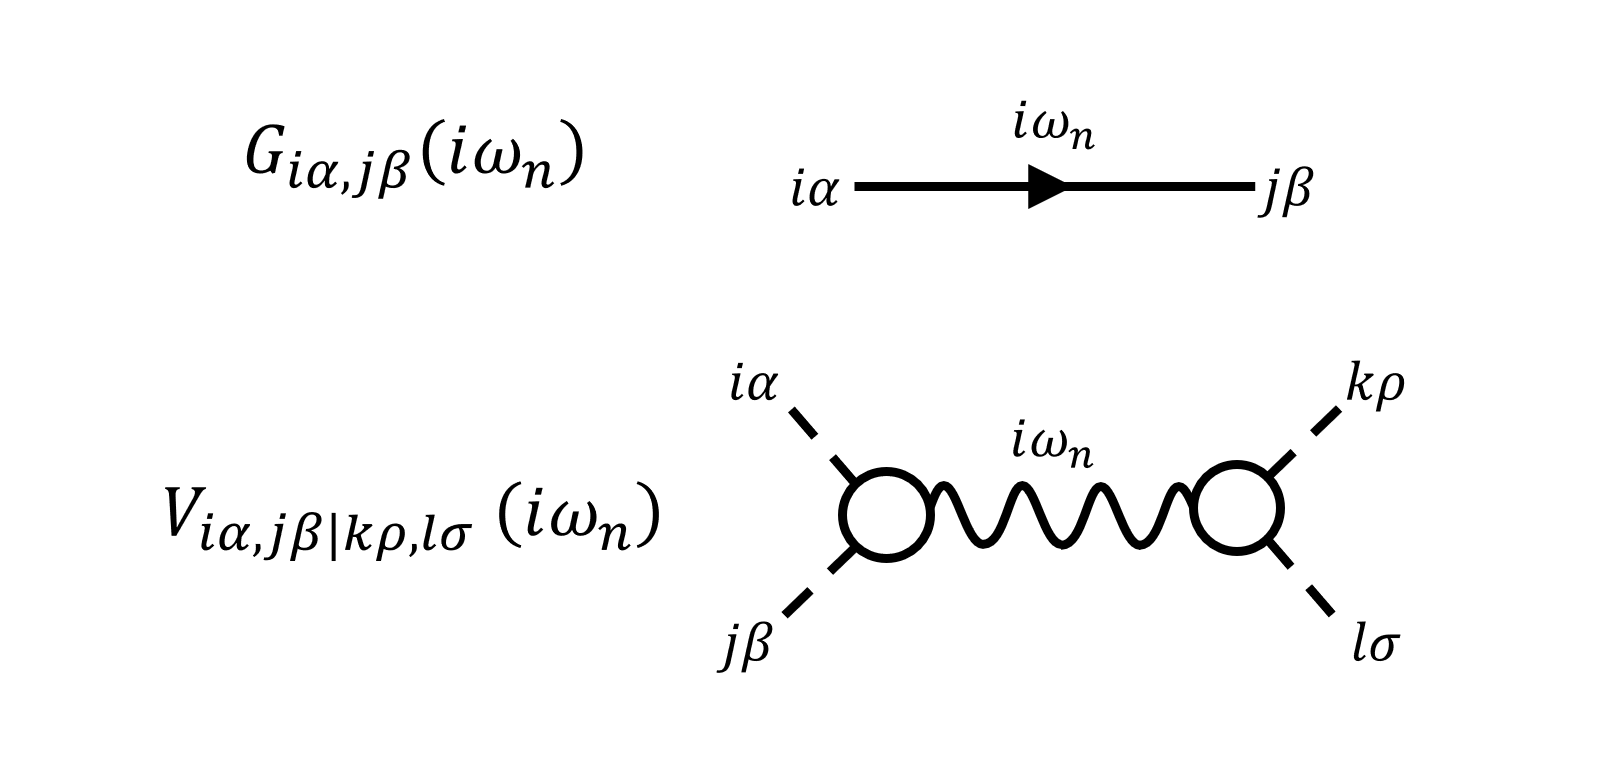
\includegraphics[width=0.8\textwidth]{Semion_diagram_elements.png}
	\caption{Графические изображения для семионной диаграммной техники.}	
\end{figure}

Задача исследования равновесной термодинамики гамильтониана \eqref{eq:Ham_semion} может быть  описана непосредственно через стандартную Мацубаровскую диаграммную технику \cite{AGD} со следующими правилами:
\begin{itemize}
	\item выражении для функции Грина невзаимодействующих семионов
	\begin{equation}
	\label{eq:Semion_Green_function}
	\begin{split}
		G_{i\alpha,j\beta}(i\omega_n) & := \left\langle T_\tau \left\{ c_{i\alpha} c^\dagger_{j\beta} \right\} \right\rangle 
		\equiv \delta_{ij} \left( i\omega_n - \xi_i \sigma^z_{\alpha\beta} + \mu_0 \right)^{-1} = \\ & = \delta_{ij} \frac{ i\omega_n +\mu_0 + \xi_i \sigma^z_{\alpha\beta} }{ \left( i\omega_n +\mu_0 \right)^2 - \xi_i^2 }
	\end{split}
	\end{equation}Традиционно, многочастичные функции Грина могут быть выражены через двухчастичную с помощью теоремы Вика.
	
	\item Выражение для вершины взаимодействия
	\begin{equation}
		\label{eq:Semion_interaction_vertex}
		V_{i\alpha, m\beta|j\rho, n\eta}(i\omega_n) = - \frac{2 g}{K} \cdot \delta_{im} \delta_{jn} J_{ij} \frac{1}{4} (\sigma^x_{\alpha \beta} \sigma^x_{\rho \eta} + \sigma^y_{\alpha \beta} \sigma^y_{\rho \eta}) \cdot \theta\left( \varepsilon_0 - |\omega_n| \right)
	\end{equation}
	где $J_{ik}$ -- матрица смежности $K$-регулярного графа, на котором определена задача. Зависимость от частоты диктуется Куперовской природой взаимодействия и отражает тот факт, что характерные передачи энергии не превышают $\varepsilon_0$, что и отражает наличие $\theta$-функции Хевисайда.
	
	\item В каждой точке встречи линий по всем индексам производится свёртка: суммирование латинских индексов по всем узлам и свёртка по спиновым греческим индексам.
	
	\item В точках соединения линия выполняется закон сохранения Мацубаровских частот: сумма всех исходящих равна сумме всех входящих. По незафиксированным законами сохранения и не относящимся ко внешним линиям диаграммы частотам происходит суммирование.
	
	\item Вычисление разновременных корреляторов различных операторов производится стандартным образом --- выражением этих корреляторов через многочастичные функции Грина и подсчётом соответствующей диаграммы.
\end{itemize}
Графические обозначения элементов техники представлены на Рис. \ref{fig:Semion_diagram_technique}.

\subsubsection{Учёт параметра порядка в семионной диаграммной технике}
У Мацубаровской техники в исходной редакции есть существенный недостаток: она плохо отражает  качественную перестройку основного состояния, происходящую при сверхпроводящем переходе. Однако, ситуацию можно исправить, воспользовавшись идеей в духе среднего поля. Именно, рассмотрим стандартную диаграммную технику Мацубары для гамильтониана \eqref{eq:Ham_semion_with_self_consistency}, но теорию возмущений будем строить по новому гамильтониану взаимодействия $H^F_{int}$. В таком случае, выражения \eqref{eq:Semion_Green_function} и \eqref{eq:Semion_interaction_vertex} изменятся, соответственно, следующим образом:
\begin{equation}
	\label{eq:Semion_Green_function_with_OP}
	\begin{split}
		G_{i\alpha,j\beta}(i\omega_n) & = \delta_{ij} \left( i\omega_n - \xi_i \sigma^z_{\alpha\beta} - \sum_k \widetilde{\Delta}^k_i \sigma^k_{\alpha\beta} + \mu_0 \right)^{-1} = \\ & = \delta_{ij} \frac{ i\omega_n +\mu_0 + \xi_i \sigma^z_{\alpha\beta} - \sum_k \widetilde{\Delta}^k_i \sigma^k_{\alpha\beta} }{ \left( i\omega_n +\mu_0 \right)^2 - \xi_i^2 - \left| \widetilde{\Delta}_i \right|^2 }
	\end{split}
\end{equation}
\begin{equation}
	\label{eq:Semion_interaction_vertex_with_OP}
		V_{i\alpha, m\beta|j\rho, n\eta}(i\omega_n) = - \frac{2 g}{K} \cdot \delta_{im} \delta_{jn} J_{ij} \cdot \sum_k \frac{1}{4} \left( \sigma^k_{\alpha \beta} - \mathcal{C}^k_i \delta_{\alpha\beta} \right) \left( \sigma^k_{\rho \eta} - \mathcal{C}^k_j \delta_{\rho\eta} \right)
\end{equation}
где $\widetilde{\Delta}$ --- параметр порядка, определяемый из уравнения самосогласования \eqref{eq:Order_paramter_self_consistency}, а $\mathcal{C}$ --- все то же термодинамическое среднее для задачи спина в постоянном магнитном поле, определяемом значением $\widetilde{\Delta}$. Постоянное слагаемое $E^F_0$ является температурно-зависимой сдвижкой энергии, так что его наличие влияет аддитивным образом лишь на свободную энергию и её температурные производные. Кроме перечисленных выше модификаций, правила техники не изменяются. 

Эта техника работает по параметру $1/K$, и является последовательным способом выяснять степень применимости седлового приближения.

\subsubsection{Диаграммная техника для поля параметра порядка}
Другим способом исследовать задачу является рассмотрение диаграммного ряда теории возмущений непосредственно для пропагатора флуктуаций параметра порядка. Изложение этой техники в формализме диаграммной техники Келдыша имеется в \cite{Kiselev_Oppermann_2000}.
\begin{enumerate}
	\item Определим флуктуацию следующим образом:
	\begin{equation}
	\label{eq:Order_paramter_fluctuation_definition}
	r^k_i(\tau) := \Delta^k_i(\tau) - \widetilde{\Delta}^k_i
	\end{equation}
	где $\widetilde{\Delta}$ --- параметр порядка, определяемый из уравнения \eqref{eq:Order_paramter_self_consistency}.
	
	\item Используя формулу
	$$
	\ln \det \left( L_0 + \delta L \right) = \ln \det L_0 + \ln \det \left( 1 + L_0^{-1} \delta L \right)
	$$
	бозонное действие \eqref{eq:Boson_action} можно переписать в виде:
	\begin{align*}
	\mathcal{A}_{b} \left[ \Delta \right] & = \mathcal{A}_{b} \left[ \widetilde{\Delta} \right] + \int\limits_{0}^{\beta} d\tau \left[ 2 \left(\frac{K}{2g}\right) \sum_{ij} \sum_k r^k_i J^{-1}_{ij} r^k_j \right] - \ln \det \left( 1 + G \delta L \right) \\
	\delta L & = - \sum_i \sum_k \sigma^k_{\alpha\beta} r^k_i \\
	\end{align*}
	где оператор $L_0^{-1}$ есть функция Грина семионной задачи с учётом параметра порядка \eqref{eq:Semion_Green_function_with_OP}.
	
	\item Далее, используя тождество
	$$
	\ln \det (1 + A) = \Tr \ln (1 + A) \equiv \sum_{n = 1}^\infty \frac{(-1)^{n-1}}{n} \Tr \left[A^n\right]
	$$
	перепишем $r$-зависимую часть действия в форме
	\begin{equation*}
	\mathcal{A}_b[r] = \int\limits_{0}^{\beta} d\tau \left[ 2 \left(\frac{K}{2g}\right) \sum_{ij} \sum_k r^k_i J^{-1}_{ij} r^k_j \right] - \sum_{n = 1}^\infty \frac{1}{2n} \Tr \left[- \left(L_0^{-1} \delta L \right)^n\right]
	\end{equation*}
	где учтено, что все нечётные порядки старше первого в сумме обнулятся после взятия функционального интеграла в силу нечётности по полям $r$. Обращение в нуль первого порядка этого ряда эквивалентно выполнению уравнения самосогласования \eqref{eq:Order_paramter_self_consistency} по определению.
	
	\item Наконец, заметим, что выражение под знаком суммы имеет очевидную интерпретацию в терминах Мацубаровской диаграммной техники с учётом параметра порядка, описанной выше: диаграмма, соответствующая выражению $F_n[r] := \Tr \left[- \left(L_0^{-1} \delta L \right)^{2 n}\right]$,  показана на Рис. \ref{fig:n_particle_renormed_vertex}. Она представляет из себя отклик $n$-го порядка на переменное внешнее поле. 
	\begin{figure}[h]
		\label{fig:n_particle_renormed_vertex}
		\centering
		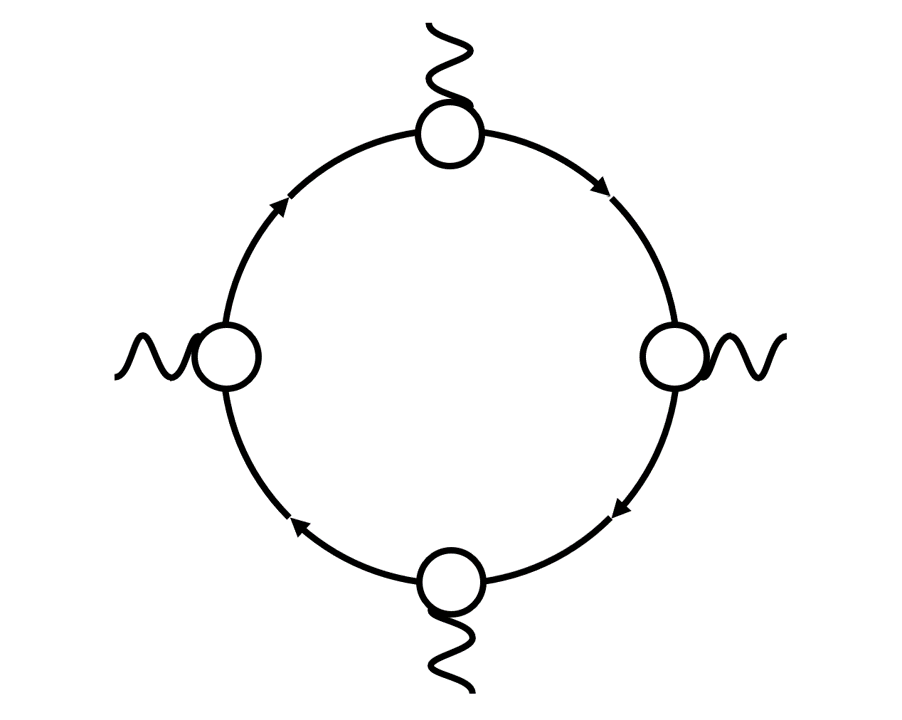
\includegraphics[width=0.5\textwidth]{N_particle_renormed_vertex.png}
		\caption{Диаграммное представление для слагаемого $n$-го порядка в действии, обозначенного в тексте как $F_n[r]$. На рисунке $n = 2$.}
	\end{figure}
	Определим также ядро этого отклика $R[n]_{ij}^{mn}\left(\tau_1,...\tau_{2n}\right)$, даваемое диаграммой на Рис. \ref{fig:n_particle_renormed_vertex}, но с усечёнными бозонными концами (т. е. просто фермионной петлёй с $2n$ вершинами в виде операторов спина). Очевидно, $R[n]$ зависит лишь от разностей времён, т. е. от $2n-1$ переменных.
	%TODO: PROP make a better description of R[n] diagram
	
	\item Таким образом, пока что полученная диаграммная техника представляет из себя задачу изучения бозонного поля с многочастичным взаимодействием. При этом следует явно отщепить слагаемое с $n = 1$, которое даёт вклад непосредственно в пропагатор поля флуктуаций $r$. Поскольку квадратичная часть действия в функциональном интеграле однозначно определяется обратной функции Грина невозмущенной задачи, то имеем тогда для пропагатора:
	\begin{equation}
	\label{eq:Order_parameter_fluctuations_propagator_definition}
		\begin{split}
			D^{mn}_{ij}(\tau) & := \left\langle T_\tau \left\{ \delta^k_i(\tau_0)    	\delta^k_i(\tau_0 + \tau) \right\} \right\rangle = \\
			& = \left[ 2 \times \frac{K}{2g} J_{ij}^{-1} \delta^{mn} - 2 \times \frac{1}{2} R[1]_{ij}^{mn}(\tau) \right]^{-1}
		\end{split}
	\end{equation}
	
	\item Итоговая диаграммная техника формулируется в терминах элементов $D$ и $R[n]$: $k$-ый порядок теории возмущении соответствует сумме всевозможных диаграмм, составленных из семионных петлей с различным чётным числом вершин $2k$ и флуктуационных пропагаторов \eqref{eq:Order_parameter_fluctuations_propagator_definition}, соответствующих волнистой линии в исходной Мацубаровской диаграммной технике для семионов. Каждая семионная петля порядка $2k$ при этом имеет дополнительный коэффициент $1/{2k}$.
\end{enumerate}  

Отметим, в частности, что обрезание теории возмущений на 4-ом порядке, что означает учёт единственной диаграммы с вершиной $\frac{1}{4}R[2]$, соответствует формализму теории Гинзбурга Ландау. Таким образом, величина петель $R[n]$ на нулевой переданной частоте задаёт коэффициенты функционала Гинзбурга-Ландау. При этом, как и раньше, тензорная инвариантность, которой по построению обладают все диаграммы, напрямую связана с калибровочной $U(1)$-инвариантностью задачи сверхпроводимости.


\subsection{Некоторые заключительные физические замечания}
Важным физическим примечанием будет соответствие полученных результатов общепринятой картине описания сверхпроводимости как нарушения зарядовой $U(1)$-симметрии: компоненты введённого бозонного векторного поля соответствуют действительной и мнимой части комплексного параметра порядка, рассматриваемого в теории сверхпроводимости. В частности, такая картина хорошо соотносится с очевидной вращательной инвариантностью полученного уравнения самосогласования \eqref{eq:Order_paramter_self_consistency}. Например, в данную теорию легко ввести внешнее электромагнитное поле методом минимального спаривания. Краткое обсуждение соответствия симметрийных аспектов теории имеется в работе \cite{Poboiko_Feigelman_Paraconductivity}.

Следующим важным физическим комментарием будет вопрос о критерии применимости метода стационарной фазы, формализма среднего поля и прочих родственных вещей. Строго говоря, все эти методы работают по параметру $1/K$, и в общем случае необходимо следить за взаимодействиями эффектов одного порядка при попытках выяснять поправки к среднеполевым ответам. Качественно, отклонения от среднеполевой картины появляются за счёт двух эффектов:
\begin{itemize}
	\item Флуктуаций параметра порядка вокруг своих средних, определяемые конечным числом соседей. Эти явления мы опишем далее.
	
	\item Эффекты неоднородностей, вносимые распределением энергий $\xi_i$ на узле, которые также уменьшаются с увеличением числа соседей. Влияние этих неоднородностей сказывается на этапе решения уравнения самосогласования, и потому их учёт является отдельной сложной задачей.
\end{itemize}
Предел $K \rightarrow \infty$, как показано в уравнении \eqref{eq:Order_parameter_self_consitency_BCS_limit}, соответствует стандартной модели БКШ, в рамках которой в системе развивается однородный параметр порядка, а все термодинамические характеристики системы, согласно теореме Андерсона, испытывают влияние беспорядка исключительно за счёт изменения одночастичной плотности состояний.

Наконец, заметим, что полученные результаты могут быть также воспроизведены с помощью формализма аномальных средних Намбу-Горькова, изложенного, например, в \cite{AGD}. Между этим и приведённым в данной работе формализмом имеется простое соответствие: средние операторов $s^{x,y}$ на узле соответствуют Горьковских аномальным средним вида $\left\langle a^\dagger a^\dagger \right\rangle$ в исходной задаче взаимодействующих электронов, в то время как оператор $s^z$ несёт информацию о диагональной части функции Грина и, соответственно, средних вида $\left\langle a^\dagger a\right\rangle$. 



%\section{Исследование решения уравнения самосогласования}
%TODO: DERIVE subsubsection{1/K-диграммная техника для параметра порядка} -- если она вообще существует



\section{Изучение свойств низкоэнергетических мод}
Нашей задачей будет изучение низкоэнергетических возбуждений над основным состоянием системы при низкой температуре $T << T_c$. При этом мы считаем, что этих возбуждений при низких температурах очень мало, а потому их взаимодействием можно пренебречь, что соответствует рассмотрению в функциональном интеграле только квадратичной по флуктуациями части бозонного действия. В таком случае, возбуждения  описываются своим пропагатором \eqref{eq:Order_parameter_fluctuations_propagator_definition}, который очевидным образом содержит все одночастичные свойства этих возбуждений.

\subsection{Связь свойств флуктуаций с их функцией Грина}
\subsubsection{Локальная плотность состояний}
В первую очередь, нас интересует статистика локальной плотности состояний на узле $\rho_i(\omega)$ этих возбуждений при низких частотах. Определение этой величины и ее связь с функцией Грина следующие:
\begin{equation}
	\label{eq:LDoS_through_GF}
	\rho_i(\omega)  := \lim_{M \rightarrow \infty} \sum_i \sum_\alpha \left| \psi^\alpha_i \right|^2 \delta(\omega - \varepsilon^\alpha) =  \lim_{\gamma \rightarrow +0} \lim_{M \rightarrow \infty} \frac{1}{\pi} \Im D_{ii}(\omega + i \gamma)
\end{equation}
где $\varepsilon^\alpha$ -- энергия возбуждения с волновой функцией $\psi^\alpha$, а также введено инфинитезимальное уширение уровней $\gamma$, отвечающее за корректный переход к термодинамическому пределу $M \rightarrow \infty$ или, эквивалентно, за регуляризацию входящей в определение локальной плотности состояний $\delta$-функции от энергии.

Как следует из определения, $\rho_i$ показывает вероятность наличия на данном узле состояния с заданной энергией $\omega$. В частности, именно эта величина будет определять исход эксперимента по туннельной микроскопии (а точнее, её среднее на масштабе порядка размера иглы). Очевидно, что в металлической системе эта величина совпадает со стандартной плотностью состояний, которая в нашей модели задаётся беспорядком и равна $1/2$. 

Важно, однако, отметить, что с интерпретацией этой величины как буквально локальной \textit{в реальном пространстве} плотности состояний следует быть осторожным, поскольку определённая в \eqref{eq:LDoS_through_GF} величина является плотностью состояний \textit{на одном узле графа}, который, в свою очередь, соответствует одноэлектронному локализованному состоянию, занимающему некоторый конечный корреляционный объём. При этом взаимное пространственное расположение различных состояний, соответствующее различным узлам графа, является отдельной задачей, поэтому физический смысл эта величина имеет лишь как среднее по масштабу меньше или порядка локализационного объёма $V_{loc}$.

\subsubsection{Inverse Participation Ratio}
Ещё одной характеристикой возбуждений, статистика которой нас будет интересовать, является т. н. Inverse Participation Ratio (далее IPR), характеризующая объём, который занимает соответствующая волновая функция. Её формальное определение и связь со свойствами функции Грина выглядят следующим образом:
\begin{equation}
	\label{eq:IPR_through_GF}
	L(\omega) := \lim_{M \rightarrow \infty} \sum_i \sum_\alpha \left| \psi^\alpha_i \right|^4 \delta(\omega - \varepsilon^\alpha) = \lim_{\gamma \rightarrow +0} \lim_{M \rightarrow \infty} \frac{\gamma}{\pi} \left| D_{ii}(\omega + i \gamma) \right|^2 
\end{equation}
Как буквально следует из определения, эта величина содержит в себе информацию о втором моменте амплитуды волновой функции, усреднённом по всем узлам системы $i$ и всем состояниям $\alpha$  с заданной энергией $\omega$.

Основным свойством IPR является то, что в термодинамическом пределе $m \rightarrow 0$ она равна 0, если состояния делокализованы, и некоторому конечному числу $\sim V_{loc}^{-1} $, если у состояний имеется конечный локализационный объём $V_{loc}$. 

Здесь также следует отметить, что нужно с осторожностью интерпретировать эту величину как характеристику структуры возбуждений в реальном пространстве из-за сложного взаимного расположения одночастичных электронных состояний, соответствующих различным узлам графа. Однако, у этой величины, тем не менее, имеется конкретный физический смысл: поскольку локализация в пространстве узлов по построению модели означает локализацию в реальном пространстве в конечном объёме $\sim V_{loc}$, то возбуждения с таким свойством не будут непосредственно приводить к диссипации энергии.


\subsection{Выражение для пропагатора флуктуаций параметра порядка}
Для начала установим явный вид пропагатора флуктуаций. Схожие вычисления в формализме диаграммной техники Келдыша можно найти в работе \cite{Poboiko_Feigelman_Paraconductivity}. 
Явный вид фермионной петли $R[1]$:
\begin{equation*}
	\begin{split}
		R[1]_{ij}^{mk}(i\omega_n) & = -T \sum_{\epsilon_n} \left[ G_{i\alpha,j\beta}(i\omega_n + i \epsilon_n) \frac{1}{2}\sigma^m_{\beta\rho} G_{j\rho,i\eta}(i \epsilon_n) \frac{1}{2} \sigma^m_{\eta\alpha} \right] = \\
		& = -\frac{1}{2} \delta_{ij} \frac{\tanh(\beta h)}{2 h} \left[ -\frac{ h^2 \delta^{mk} }{ h^2 + \frac{\omega_n^2}{4} } + \frac{ \omega_n h^s \epsilon^{smk} + 2 h^m h^k - h^2 \delta^{mk} }{h^2 + \frac{\omega_n^2}{4}} \right]
	\end{split}
\end{equation*}
где
$$
h^x_i = \widetilde{\Delta}^x_i, h^y_i = \widetilde{\Delta}^y_i, h^z_i = - \xi_i, h^2 = \left| \widetilde{\Delta}_i \right|^2 + \xi_i^2
$$
Обращаем внимание, что частотный аргумент петли и пропагатора $\omega_n$ представляет из себя бозонной Мацубаровскую частоту, а внутренняя частота петли $\varepsilon_n$ --- фермионную. Используя формулу \eqref{eq:Order_paramter_fluctuation_definition}, выпишем явный вид обратного пропагатора:
\begin{equation}
	\label{eq:Order_parameter_fluctuation_inverse_propagator_explicit}
	\begin{split}
		\left[ D^{mk}_{ij}(i \omega_n) \right]^{-1} & =  2\left[ \frac{K}{2g} J_{ij}^{-1} \delta^{mk} - \frac{1}{2} R[1]_{ij}^{mk}(i\omega_n) \right] = \\
		& = \frac{K}{g} J_{ij}^{-1} \delta^{mk} + \delta_{ij} \frac{\tanh(\beta h)}{h} \left[ \frac{ h^m h^k - h^2 \delta^{mk} }{h^2 + \frac{\omega_n^2}{4}} + \frac{ \frac{\omega_n}{2} h^s \epsilon^{smk} }{h^2 + \frac{\omega_n^2}{4}} \right]
	\end{split}
\end{equation}
Симметричная по $m,k$ часть этого выражения содержит в себе информацию о функции Грина двух мод флуктуаций: поперечной и продольной, соответственно тому, как направления колебаний соотносятся с направлением параметра порядка. В терминах комплексного параметра порядка это соответствует фазовой моде Голдстоуна и амплитудной моде Хиггса. Недиагональный же член несёт в себе информацию о смешивании двух мод между собой.

Заметим, что \textit{всегда} имеется хотя бы одно поперечное возбуждение с $\omega = 0$, поскольку оно является следом нарушенной $U(1)$-симметрии: уравнение самосогласования \eqref{eq:Order_paramter_self_consistency} инвариантно относительно этой симметрии, и в частности, относительно инфинитезимально малых поворотов параметра порядка на некоторый угол без изменения модуля, что и соответствует описанному возбуждению.


\subsection{Итоговая задача изучения низкоэнергетических поперечных мод}
Чтобы сделать задачу более конкретной, примем ряд дальнейших упрощений:
\begin{enumerate}
	\item Поскольку нас интересуют низкоэнергетические моды, то далее будем считать $\omega_n \ll |\Delta|$. Как следствие, взаимодействием продольной и поперечной мод можем пренебречь
	\item В рамках теории сверхпроводимости для чистого металла, Хиггсовская мода должна быть массивной, что соответствует наличию щели в низкоэнергетическом спектре продольных возбуждений. Некоторые расчёты, качественно обосновывающие данное приближение, имеются в работе \cite{Shtyk_Feigelman_2017}. Поэтому мы будем считать, что такая картина сохраняется и далее, так что в дальнейшем будем изучать только поперечную моду. 
	\item Также сделаем одно упрощение, касающееся статистики поля параметра порядка $\widetilde{\Delta}$. Для дальнейших расчётов мы будем считать, что его значение на каждом узле \textit{равно своему значению в пределе теории БКШ \eqref{eq:Order_parameter_BCS_limit}}. Мотивация этого приближения состоит в следующем: 
	\begin{enumerate}
		\item[а.] ранее для этой задачи уже были проведены оценки типичных значений $K$, при которых будет происходить основная физика \cite{FI_microwave}. Мы ещё вернёмся к этим оценкам.
		\item[б.] Эти оценки, по данным \cite{Feigelman_et_al_2010}, лежат в области, где параметр порядка флуктуирует довольно слабо. 
	\end{enumerate}
	Таким образом, роль беспорядка в этом приближении сводится только к непосредственному влиянию величин $\xi_i$, явным образом входящего в выражение петли $R[1]$, определяющей флуктуационный пропагатор \eqref{eq:Order_parameter_fluctuation_inverse_propagator_explicit}. Сделаем пару важных замечаний:
	\begin{enumerate}
		\item[а.] строго говоря, это приближение не вполне обоснованно, так как лидирующий порядок изучаемых эффектов есть $1/K$, равно как и порядок флуктуаций параметра порядка. Однако мы надеемся, что качественная картина от этого не изменится. В дальнейшем это приближение будет явно проверено.
		\item[б.] Важным замечанием является также и то, что игнорирование истинного распределения параметра порядка приводит к потере симметрийной поперечной моды с $\omega = 0$, описанной ранее.
	\end{enumerate}
\end{enumerate}

Теперь можно дать окончательную формулировку задачи, которую мы собираемся далее решать, и которая должна описывать появление в сверхпроводнике низкоэнергетических возбуждений. А именно, мы хотим выяснить статистику локальной плотности состояний \eqref{eq:LDoS_through_GF} и IPR \eqref{eq:IPR_through_GF} собственных мод \textit{на нулевой энергии} для линейного оператора 
\begin{equation}
	\label{eq:Investigated_linear_operator}
	A_{ij}(\omega) = \frac{K}{g} J_{ij}^{-1} - \delta_{ij} \eta_i (\omega)
\end{equation}
где величина $\eta_i$ определяется формулой
\begin{equation}
	\label{eq:eta_definition}
	\eta_i(\omega) = \frac{ \sqrt{ |\Delta_i|^2 + \xi_i^2 } }{ |\Delta_i|^2 + \xi_i^2 - \frac{\omega^2}{4} }
\end{equation}
а величины $\Delta_i$ все являются одинаковыми и задаются как параметр модели формулой \eqref{eq:Order_parameter_BCS_limit}. Поясним, что нас интересует именно нулевое собственное значение, так как, согласно формулам \eqref{eq:LDoS_through_GF}-\eqref{eq:IPR_through_GF}, вся информация содержится буквально в операторе $A^{-1}$, что соответствует его функции Грина $G(E) = (E - A)^{-1}$ именно при $E = 0$. Реальная физическая энергия возбуждений входит в задачу как параметр $\omega$.


\subsection{Основные изучаемые характеристики ансамбля}
Напомним, что в конечном итоге мы интересуемся статистическими свойствами ансамбля, задаваемого присутствующими в определении \eqref{eq:Investigated_linear_operator} случайностями. Для этого удобно ввести две величины, в значительной степени характеризующие распределение -- среднее и типичное значение:
$$ x_{mean} := \langle x \rangle $$
$$ x_{typ} := \exp \langle \ln x \rangle $$
где $\langle \cdot \rangle$ означает усреднение по ансамблю. Эти величины обладают следующими качественными свойствами:
\begin{itemize}
	\item среднее значение, как известно благодаря центральной предельной теореме, характеризует то, как устроены самоусредняющиеся в реальном образце аддитивные величины.
	\item В тоже время типичное значение характеризует те вещи, которые являются существенно локальными, и потому чувствительны к конкретной реализации. Математически это выражается в том, что, поскольку логарифм -- медленная функция, то типичное значение, согласно своему названию, будет близко к положению максимума функции распределения, т. е. к значению, которое будет реализовываться чаще всего.
\end{itemize}


\subsection{Связь поставленной задачи с локальными свойствами}
К сожалению, поставленная задача об исследовании функции Грина оператора \eqref{eq:Investigated_linear_operator} обладает тем недостатком, что она нелокальна по узлам: в общем случае матрица $J^{-1}$ имеет большое число ненулевых матричных элементов, так что каждый узел исходного графа связан с большим число других узлов, в том числе находящихся от него на большом расстоянии по графу. Однако, если интересоваться лишь фактом \textit{наличия} конечной в термодинамическом пределе плотности возбуждений, то оказывается, что задачу можно свести к локальной. Делается это следующим образом:
\begin{enumerate}
	\item Обозначим
	$$
	\hat{\eta}_{ij} = \delta_{ij} \eta_i, \hat{R}_{ij} = \frac{g}{K} J_{ij}
	$$
	Также введём оператор
	\begin{equation}
		\label{eq:Local_operator_definition}
		\hat{C} = \sqrt{\hat{\eta}} \hat{R} \sqrt{\hat{\eta}}
	\end{equation}
	и его функцию Грина на собственном значении $1$ с некоторым уширением уровней:
	\begin{equation}
		\label{eq:Local_operator_Green_function_definition}
		\hat{G}(\gamma) = \left( \left[ 1 + i \gamma \right] - \hat{C} \right)^{-1} 
	\end{equation}
	Под числами здесь подразумеваются соответствующие скалярные матрицы, пропорциональные единичной.
	Далее будет продемонстрировано, что интересующая нас задача может быть сведена к исследованию \textit{локального} оператора $\hat{C}$ и его функции Грина $\hat{G}$
	\item Проделаем следующие преобразования над флуктуационным пропагатором $D$:
	\begin{equation}
		\label{eq:Connection_between_GF}
		\begin{split}
			D(\gamma \rightarrow +0) & \equiv \left( \hat{A} + i 0 \right)^{-1} \overset{\eqref{eq:Investigated_linear_operator}}{=} \left( \hat{R}^{-1} - \hat{\eta} + i 0 \right)^{-1} \equiv \\
			& \equiv \sqrt{\hat{\eta}} \hat{R}  \left( \sqrt{\hat{\eta}} \hat{R} \sqrt{\hat{\eta}} - \sqrt{\hat{\eta}} \hat{R} \left[ \hat{\eta} - i 0 \right] \hat{R} \sqrt{\hat{\eta}} \right)^{-1} \hat{R} \sqrt{\hat{\eta}} = \\
			& = \hat{C} \hat{\eta}^{-1/2} \left( \hat{C} - \hat{C}\left[1 - i 0 \hat{\eta}^{-1} \right] \hat{C} \right)^{-1} \hat{\eta}^{-1/2} \hat{C} = \\
			& = \hat{C} \hat{\eta}^{-1/2} \underset{\hat{G}(+0)}{\underbrace{  \left( \left[1 - i 0 \hat{\eta}^{-1} \right]^{-1} - \hat{C} \right)^{-1}  }} \left[1 - i 0 \hat{\eta}^{-1} \right]^{-1} \hat{C}^{-1} \hat{\eta}^{-1/2} \hat{C} = \\
			& = \left/ \hat{\eta}^{-1} > 0 \right/ = \hat{C} \hat{\eta}^{-1/2} \hat{C}^{-1} \hat{C} \hat{G}(+0) \hat{C}^{-1} \hat{\eta}^{-1/2} \hat{C} = \\
			& = \left/ \hat{C} = 1 + i0 - \hat{G}(+0)^{-1} \right/ = \\
			& = \hat{C} \hat{\eta}^{-1/2} \hat{C}^{-1} \left( \hat{G}(+0) - 1 \right) \hat{C}^{-1} \hat{\eta}^{-1/2} \hat{C}
		\end{split}
	\end{equation}
	При преобразованиях использовалось условие $\hat{\eta} > 0$, означающее положительную определённость соответствующей матрицы. Также операторы $\hat{R}, \hat{\eta}$ считались обратимыми: матрица $\hat{\eta}$ и все её ненулевые степени обратимы из-за положительной определённости, а обратимость матрицы $\hat{R} \propto J$ уже обсуждалась ранее.
	
	\item В таком случае, для локальной плотности состояний возбуждений верно следующее:
	\begin{equation}
		\label{eq:Connection_of_LDoS_with_Im_part_of_local_GF}
		\begin{split}
			\rho_i & \equiv \frac{1}{\pi} \Im \left\langle i \right| D \left| i \right\rangle = \frac{1}{\pi}\Im \left\langle i \right| \hat{C} \hat{\eta}^{-1/2} \hat{C}^{-1}  \left( \hat{G}(+0) - 1 \right) \hat{C}^{-1} \hat{\eta}^{-1/2} \hat{C} \left| i \right\rangle = \\
			& = \left/ \hat{C}_{ij}, \hat{\eta}_{ij} \in \mathbb{R} \right/ = \left\langle i \right| \hat{C} \hat{\eta}^{-1/2} \hat{C}^{-1} \left[ \frac{1}{\pi}\Im \hat{G}(+0) \right] \hat{C}^{-1} \hat{\eta}^{-1/2} \hat{C} \left| i \right\rangle = \\
			& =  \left/ C^{-1} \left[ \Im \left(\lambda + i0 - C \right)^{-1} \right] C^{-1} = \frac{1}{\lambda^2} \left[ \Im \left(\lambda + i0 - C \right)^{-1} \right] \right/ = \\
			& = \left\langle i \right| \hat{C} \hat{\eta}^{-1/2} \left[ \frac{1}{\pi}\Im \hat{G}(+0) \right] \hat{\eta}^{-1/2} \hat{C} \left| i \right\rangle \equiv \\
			& \equiv \frac{1}{\eta_i} \left\langle i \right| R \left[ \frac{1}{\pi}\Im \hat{G}(+0) \right] R \left| i \right\rangle
		\end{split}
	\end{equation}
	Поскольку операторы $R$ предполагаются обратимыми, то из этой формулы можно сделать следующий вывод: \textit{у исходного оператора \eqref{eq:Investigated_linear_operator} существует локальная плотность состояний тогда и только тогда, когда существует ненулевая плотность собственных состояний оператора $C$ с собственным числом 1}.
	
	\item Наконец, рассмотрим связь между IPR для двух задач. Поскольку нас интересует IPR в случае с конечной плотностью состояний, то чтобы предел $\gamma \rightarrow 0$ в определении IPR \eqref{eq:IPR_through_GF} был отличен он нуля, необходимо, чтобы малость $\gamma$ компенсировала вещественная часть функции Грина:
	\begin{equation}
		\label{eq:Condition_on_GF_real_part_for_localized_states}
		L > 0 \Rightarrow \lim_{\gamma \rightarrow 0} \lim_{M \rightarrow \infty} \left| \Re D_{ii} \right| = \infty
	\end{equation}
	В таком случае, верно следующее: \textit{свойство локализации собственных мод интересующего нас оператора \eqref{eq:Investigated_linear_operator} имеется тогда и только тогда, когда это свойство наличествует у собственных мод локального оператора \eqref{eq:Local_operator_definition} с единичным собственным числом}.
\end{enumerate}
Итогом этих рассуждения является следующее важное следствие: качественные характеристики, такие как наличие конечной плотности состояний и локализация низкоэнергетических возбуждений, задаваемых оператором \eqref{eq:Investigated_linear_operator}, можно изучать по аналогичным свойствам локального оператора \eqref{eq:Local_operator_definition}. А потому исследование может быть переведено в плоскость исследования функции Грина локального оператора \eqref{eq:Local_operator_Green_function_definition} на единичном собственном числе. 
Подчеркнём, однако, что полученное сопоставление не сохраняет численные значения, а потому, строго говоря, может потенциально вносить некоторые дополнительные параметрические зависимости в получаемые ответы.


\subsection{Качественные предсказания о поведении локальной модели}
Прежде чем приступить к исследованию новой локальной задачи, необходимо упомянуть, что задача изучения локального оператора \eqref{eq:Local_operator_definition} в интересующей нас связи была сформулирована в работе \cite{FI_microwave}, и там же был сделан ряд качественных и количественных предсказаний касательно поведения этой модели, которые мы сейчас кратко изложим. Основный их смысл состоит в наличии \textit{двух характерных значений параметра $K$} со следующими свойствами:
\begin{enumerate}
	\item Точка
	\begin{equation}
		\label{eq:K2_definition}
		K_2 = \frac{g}{4} \exp \left\{ \frac{1}{g} \right\}
	\end{equation}	
	характеризует значение $K$, начиная с которого (при движении из бесконечных $K$) в системе появляются низкоэнергетические моды со сколь угодно низкой энергией.
	\item Точка
	\begin{equation}
		\label{eq:K1_definition}
		K_1 = g \exp \left\{ \frac{1}{2g} \right\}
	\end{equation}
	характеризующая момент, начиная с которого (при движении из бесконечных $K$) возбуждения со сколь угодно низкой энергией становятся делокализованными.
	\item В работе также исследована асимптотика положения этих точек на малых частотах $\omega \ll \Delta$. Утверждается, что она может быть описана как
	$$
	K_1(\omega) = K_1(0) \left(1 + \frac{1}{\sqrt{6}g} \frac{\omega}{2 \Delta} \right)
	$$
	$$
	K_2(\omega) = K_2(0) \left(1 + \frac{1}{2} \frac{\omega^2}{4 \Delta^2} \right)
	$$
\end{enumerate}
Заметим также, что с учётом результатов по исследованию поведения уравнения самосогласования \eqref{eq:Order_paramter_self_consistency} вблизи $T_c$, проведённого в работе \cite{Feigelman_et_al_2010}, предсказывается следующая картина при уменьшении $K$:
\begin{itemize}
	\item при достижении $K = K_2 \gg 1$ (самый большой масштаб для $K$ в задаче) появляются низкоэнергетические возбуждения. Но на момент появления они ещё локализованы, и поэтому не приводят к диссипации.
	\item При достижении $1 \ll K = K_1 \ll K_2$ низкоэнергетические моды делокализуются. Одновременно с этим, беспорядок вносит сильную неоднородность в поле параметра порядка, делая одноузельное распределение величины $\Delta$ по узлам крайне широким, так что в этой области приближение $\Delta = \const$ перестаёт быть применимым.
	\item Наконец, при достижении некоторого критического значения $1 \ll K = K_c \ll K_1$ беспорядок вносит критическую неоднородность в распределение параметра порядка, что разрушает сверхпроводящее состояние.
\end{itemize}
Таким образом, интересующая нас область $K \ge K_1$, которую должна описывать исследуемая нами модель, согласно этим предсказаниям, правильно описывает наблюдаемую экспериментально качественную картину. Дальнейшее исследование, проделанное в данной работе, в первую очередь проверяет сделанные выше утверждения.
\chapter{Алгоритм численного исследования упрощённой модели}  \label{Numer}
К сожалению, авторами не придумано аналитического способа решения поставленной задачи в терминах операторов \eqref{eq:Investigated_linear_operator} или даже \eqref{eq:Local_operator_definition}. Однако стремление исследовать локальную задачу для функции Грина \eqref{eq:Local_operator_Green_function_definition} основано на том, что для неё существует мощный метод численного исследований вопроса, который мы далее опишем. Также этот метод позволяет исследовать статистику решения уравнения самосогласования, что нами также будет проделано.



\section{Теория алгоритма популяционной динамики}
В данной секции будет дано краткое теоретическое обоснование и формулировка численного алгоритма для исследования локальных задач на регулярных графах.


\subsection{Связь свойств большого $K$-регулярного со свойствами деревьев с постоянными числом ветвления}
Большие $K$-регулярные графы обладают следующим набором полезных свойств, которые позволяют их на физическом уровне строгости считать не содержащими циклов. Более детально, рассуждение выглядит следующим образом:
\begin{itemize}
	\item Математически строгим фактом является следующее утверждение: среднее число циклов в большом регулярном графе является некоторой константой и не зависит от его размера в термодинамическом пределе $M \rightarrow \infty$. Формально, на уровне теоремы, это выглядит так: рассмотрим последовательность ансамблей $R(M)$ случайных графов размера $M$ с заданным числом ветвления $K$. Обозначим через $\left\langle \cdot \right\rangle_M$ среднее от некоторой величины по ансамблю $R(M)$, а через $c_k$ обозначим число циклов длины $k$ в заданном графе. Тогда
	\begin{equation}
		\label{eq:Theorem_average_number_of_cycles}
		\forall k > 0 \hookrightarrow \left\langle c_k \right\rangle_M = \frac{K^k}{2k} \left(1 + o(1) \right), M \rightarrow \infty 
	\end{equation}
	Доказательство этого утверждения можно восстановить по \cite{McKay_1981}. 
	
	\item Физическая интерпретация этой теоремы состоит в том, что вероятность у случайно выбранного узла принадлежать циклу заданной длины в термодинамическом пределе равна нулю: действительно, число узлов, лежащих в каком-нибудь цикле длины $k$ в термодинамическом пределе является постоянным числом $K^k / 2$, так что доля таких узлов во все системе исчезающе мала.
	
	\item Очевидным следствием будет следующее утверждение про некоторое подмножество узлов небольшого радиуса: вероятность того, что внутри этого подмножества содержится \textit{какой-либо цикл}, также равна нулю в термодинамическом пределе. Это свойство носит название \textit{локально древовидной структуры}.
	
	\item Важное физическое проявление указанного свойства состоит в том, что все физические величины, обладающие конечной характерной длиной, не будут различать достаточно большой $K$-регулярный граф и дерево с постоянным числом ветвления $K$. Такими величинами являются, например, свойства волновых функций в локализованной фазе, все характеристики конечных систем, а также все характеристики системы на конечной частоте \cite{Tikhonov_2016}.
\end{itemize}
Далее мы будем активно пользоваться этими рассуждениями, а именно, мы предположим, что в рассматриваемом нами графе нету циклов, т. е. он является деревом. Здесь необходимо сделать некоторые физические комментарии:
\begin{itemize}
	\item Разумеется, роль циклов в нелокальных свойствах весьма существенна. Например, исследование задач буквально на деревьях требует очень аккуратного обращения с граничными условиями, поскольку на дереве граница даёт доминирующий вклад в общий объём системы, в то время как на больших регулярных графах выполнение правильных граничных условий самосогласованно обеспечивается именно циклами размерами порядка диаметра системы. В частности, известно \cite{Tikhonov_2016}, что у статистики свойств состояний и уровней энергии в делокализованной фазе наблюдаются существенные качественные различие в случае дерева и регулярного графа. Поэтому в исследуемых нами системах необходимо озаботиться механизмами, гарантирующих правильное поведение подобных величин.
	
	\item Также заметим, что замена случайного регулярного графа на дерево по сути является способом избавиться от беспорядка, вносимого распределением ансамбля $K$-регулярных графов.
	
	\item Замена большого регулярного графа на дерево с постоянным числом ветвления с дополнительными условиями самосогласования также может быть рассмотрена в терминах реплично-симметричного приближения и соответствующей седловой точки некоторого функциональньного интеграла, что проделано в работе \cite{Metz_Castillo_2017}.
\end{itemize}


\subsection{Вывод уравнений популяционной динамики}
Итак, перед нами стоит задача вычисления статистики диагональных элементов функции Грина \eqref{eq:Local_operator_Green_function_definition} для оператора $C$, живущего теперь уже на дереве. Для \textit{статистики} буквально в этой задаче существует мощная численная процедура, называемая \textit{методом популяционной динамики}. Она уже неоднократно использовалась для изучения задач одночастичной Андерсоновской локализации \cite{Biroli_2010} и показала себя крайне эффективно. Далее мы продемонстрируем обоснование и некоторые полезные свойства этого метода на основании работы \cite{Rogers_2008}.

\subsubsection{Обозначения}
Примем ряд обозначений для дальнейшего изложения (большинство из них нужны лишь для записи вывода основных результатов и не потребуются для использования и обсуждения этих результатов):
\begin{enumerate}
	\item Далее мы будем обозначать одинаково граф, множество его узлов, рёбер и прочие характеристики --- из контекста всегда будет понятно, о чем идёт речь. 
	
	\item Кроме самого графа $T$ исходной системы нам также понадобится граф $T[j]$, получаемы из исходного удалением вершины $j$ (и, соответственно, всех смежных ей рёбер).
	
	\item Для нас существенен следующий факт: если граф $T$ был деревом, то все графы $T[j]$ будут набором несвязанных деревьев, каждое из которых можно быть однозначно задано своим корнем $k \in \partial j$, являющимся одним из непосредственных удалённого узла $j$ в исходном дереве. Эти новые поддеревья мы обозначим как $T[j]\{k\}$
	
	\item Далее мы будем вычислять некоторые функции $f$ для заданного графа $T$. Если это делается для графов $T[j]$ или $T[j]\{k\}$, то мы будем такие характеристики обозначать, соответственно, как $f[j], f[j]\{k\}$.
	
	\item В частности, для некоторого узла $i \in T$ графа мы будем обозначать множество его соседей как
	$$
	\left\{ k : \langle ik \rangle \in T \right\} \equiv \partial i
	$$
	Если речь будет идти о графах $T[j],T[j]\{k\}$, то границу мы будем обозначать соответственно $\partial[j]i, \partial[j]\{k\}i$
		
\end{enumerate}

\subsubsection{Определение локальных полей}
Итак, пусть у нас имеется некоторое дерево или система деревьев $T$, и нас интересуют диагональные элементы функции Грина вида
$$
G(\mu = 1 + i0)_{ii} := \left( \mu - \hat{C} \right)^{-1}_{ii} 
$$
где матрица $\hat{C}$ выражается через матрицу смежности графа $T$ посредством определения \eqref{eq:Local_operator_definition}. Для нас существенно, что у матрицы $C$ множество индексов ненулевых элементов является подмножеством множества таких индексов для матрицы смежности графа $T$. Далее дадим следующи ряд определений:
\begin{itemize}
	\item Введём на каждом узле $i$ графа некоторое вещественное поле $\phi_i \in \mathbb{R}$ и рассмотрим ансамбль значений этих полей, задаваемых следующим весом:
	\begin{equation}
	\label{eq:Cavity_method_generating_function}
	P\{\phi\} := \exp\left\{ \frac{i}{2} \left(\mu\sum_{i \in T}\phi_i^{2} - \sum_{i,j \in T} \phi_i C_{ij} \phi_j \right)\right\} 
	\end{equation}
	
	\item Определим также стат. сумму этого распределения
	\begin{equation}
	\label{eq:Cavity_method_partition_function_definition}
	Z := \int \left( \prod_{k \in T} d\phi_k \right) P\{\phi\}
	\end{equation}
	
	\item Среднее от некоторой функции значения полей $f\left( \{\phi\} \right)$ определяется как
	\begin{equation}
	\label{eq:Cavity_method_average_definition}
	\left\langle f \right\rangle = \frac{1}{Z} \int \left( \prod_{k \in T} d\phi_k \right) f\left( \{\phi\} \right) P\{\phi\} 
	\end{equation}
	Поскольку у $\mu$ имеется положительная мнимая часть, то все интегралы являются сходящимися. 
	
	\item Элементы функции Грина $G$ могут быть выражены как
	\begin{equation}
	\label{eq:Cavity_method_Green_function_expression}
	G_{ij} = i \left\langle \phi_i \phi_j \right\rangle
	\end{equation}
	
	\item Также нам понадобятся функции одноузельных распределений введённых полей, определяемые как
	\begin{equation}
	\label{eq:Cavity_method_single_field_distribution_definition}
	p_i(x) := \left\langle \delta(\phi_i - x) \right\rangle
	\end{equation}
	
	\item Очевидным свойством является то, что одноузельные распределения содержат всю интересующую нас информацию о диагональных элементах функции Грина:
	\begin{equation}
	\label{eq:Cavity_method_GF_diagonal_elements_through_single_field_distrivution}
	G_{ii} = \int p_i(y) dy
	\end{equation}
	\item Как указано в начале, все эти определения и утверждения валидны также для $T[j], T[j]\{k\}$.
\end{itemize}
Отметим, что подход производящего функционала также может быть использован для аналитического исследования некоторого класса задача на графах методом реплик, что проделано, например, в \cite{Rodgers_Bray_1988}.

\subsubsection{Рекуррентные уравнения на одноузельные распределения}
Рассмотрим функции $p[j]_i(x)$ в системе с выкинутым узлом $j$. Прежде всего, заметим, что поскольку поддеревья $\left\{ T[j]\{i\}: i \in \partial j \right\}$ не связаны между собой рёбрами, то из определения $p$ тривиально следует равенство одноузельных распределений для узлов новых поддеревьев, если эти распределение вычислять во всей системе $T[j]$ и в отдельном поддереве $T[j]\{k\}$:
$$
i \in  T[j]\{k\} \Rightarrow p[j]_i(x) \equiv p[j]\{k\}_i(x)
$$
С другой стороны, определение $p[j]$ с помощью преобразований над весом усреднения \eqref{eq:Cavity_method_generating_function} позволяет показать следующее тожество для одноузельных распределений в корнях деревьев $T[j]\{k\}$:
\begin{equation}
	\label{eq:Single_field_cavity_distribution_recurrence_relation}
	p[j]\{k\}_k(x) = \frac{\exp\left\{ \frac{i}{2}\mu x^2\right\} }{Z[j]\{k\}} \prod\limits_{s \in \partial[j]k} \left[Z[k]\{s\} \int p[k]\{s\}_s(y) \exp\left\{ -i x y С_{sk} \right\} dy \right]
\end{equation}
Аналогичным образом можно установить связь между системой $T$ и $T[j]$
\begin{equation}
	\label{eq:Single_field_distribution_though_cavity_distributions}
	p_j(x) = \frac{\exp\left\{ \frac{i}{2}\mu x^2\right\} }{Z} \prod\limits_{k \in \partial j} \left[Z[k] \int p[j]_k(k) \exp\left\{ -i x y С_{jk} \right\} dy \right]
\end{equation}

\subsubsection{Рекуррентные уравнения на диагональные элементы функции Грина}
Следующим шагом будет заметить, что уравнения \eqref{eq:Single_field_cavity_distribution_recurrence_relation}-\eqref{eq:Single_field_distribution_though_cavity_distributions} допускают следующий анзатц:
\begin{equation}
	\label{eq:Single_site_distribution_gaussian_ansatz}
	p...(x) = A... \exp\left\{- \frac{x^2}{2 v...} \right\}, v... \in \mathbb{C}
\end{equation}
где $...$ - индексы, задающие граф и узел. Данный анзатц приводит к следующим уравнениям на величины $v$:
\begin{equation}
	\label{eq:Cavity_amplitude_recurrence_relation}
	v[j]_k = \left[ \sum_{s \in \partial[j]k} C_{ks}^{2} v[k]_s - i\mu \right]^{-1}
\end{equation}
\begin{equation}
	\label{eq:Dispersion_though_cavity_amplitudes}
	v_j = \left[ \sum_{k \in \partial j} C_{jk}^{2} v[j]_k - i\mu \right]^{-1}
\end{equation}
Заметим, что поскольку $\Im \mu > 0$, то можно показать, что данные рекуррентные уравнения сохраняют свойство $\Re v > 0$, так что все рассматриваемые интегралы являются Гауссовым образом сходящимися.

Наконец, важным наблюдением будет то, что гауссов анзатц \eqref{eq:Single_site_distribution_gaussian_ansatz} напрямую связан с желаемыми диагональными элементами функции Грина посредством уравнения \eqref{eq:Cavity_method_GF_diagonal_elements_through_single_field_distrivution}:
$$
G_{jj} \equiv i v_j
$$

Введём общепринятые для полученного метода обозначения:
$$
v[j]_k =: G_{j \rightarrow k}
$$
$$
i v_j =: G_j \equiv G_{jj}
$$
Тогда метод популяционной динамики формулируется как следующий набор рекуррентных уравнений:
\begin{equation}
	\label{eq:Population_dynamics_equations}
	\begin{split}
		G_{j \rightarrow k} & = \left[ \sum_{s \in \partial[j]k} C_{ks}^{2} G_{k \rightarrow s} - i\mu \right]^{-1} \\
		G_j & = i \left[ \sum_{k \in \partial j} C_{jk}^{2} G_{j \rightarrow k} - i\mu \right]^{-1}
	\end{split}
\end{equation}
Таким образом, система уравнений \eqref{eq:Population_dynamics_equations} является замкнутым способом определить значение диагональных элементов функции Грина \eqref{eq:Local_operator_Green_function_definition} на заданном древесном графе.

\subsubsection{Комментарии по использованию полученных уравнений}
На полученные рекуррентные уравнения может смотреть двумя способами:
\begin{itemize}
	\item во-первых, как на способ найти диагональную функцию Грина на любом узле графа \textit{в заданной реализации беспорядка} и \textit{без явной диагонализации соответствующей матрицы}. Здесь важно два аспекта:
	\begin{itemize}
		\item Во-первых, такая интерпретация явным образом указывает на разницу между деревом и регулярным графом: в первом случае указанные уравнения сопровождаются указанием граничных условия, в то время как во втором требуется условие согласования на всех циклах системы.
		\item Полученная система уравнений требует двух процедур рекурсии от краёв дерева к центру и обратно, причём можно показать, что алгоритм имеет сложность и затраты памяти $O(M)$, где $M$ --- число узлов. Это даёт огромный выигрыш по сравнению с методами диагонализации разреженных матриц, которые в лучшем случае требуют $O(M^2)$ времени и памяти. 
	\end{itemize}
	\item Во-вторых, можно интерпретировать эти рекуррентные соотношения как \textit{уравнения на распределения по ансамблю беспорядка}. Более конкретно, система \eqref{eq:Population_dynamics_equations} может быть переписана в замкнутое интегральное уравнение на распределение величин $P(G_{j \rightarrow k}), P(G_i)$ при известном распределении величин $\xi_i$, организующим в системе беспорядок. Здесь тоже сделаем два важных физических замечания
	\begin{itemize}
		\item Полученные численные уравнения в таком случае являются ничем иным, как способом итеративного численного решения указанного интегрального уравнения. В связи с этим заметим также, что возникающее таким образом уравнение на стационарную точку рекурсии в реальной системе на графе является следствием упомянутых уравнения самосогласования, возникающих в результате присутствия в системе циклов размером порядка диаметра графа. 
		\item Такой подход к этим уравнениями приводит к известным результатам по описанию локализации Андерсона \cite{AAT}. Обратим внимание, что это возможно только благодаря локально древовидной структуре графа. 
	\end{itemize}
\end{itemize}

Наконец, как уже отмечено в начале этой главы, нам нужно гарантировать, что получаемые нами, вообще говоря, нелокальные свойства, вроде плотности состояний на узле и IPR будут относиться именно к $K$-регулярному графу. В общем случае (т. е. если априори неизвестно, является ли фаза локализованной) это достигается правильным порядком предельного перехода по имеющимся параметрам: числу итераций рекурсии $N$, размеру системы $M$ и уширению уровней $\gamma$. Правильный порядок предельного перехода получается, если вспомнить, что ответы для деревьев и графов не отличаются для величин с некоторым конечным масштабом длины. При конечном значении регуляризации $\gamma$ такой характерной величиной будет длина $L_{char} \propto \ln \gamma^{-1}$, которую способна пролететь частица без диссипации \cite{Tikhonov_2016}. А значит, правильный порядок таков:
\begin{itemize}
	\item сначала необходимо найти стационарную точку уравнений рекурсий, обеспечив тем самым выполнение самосогласования за счёт больших циклов,
	\item затем требуется перейти к термодинамическому пределу бесконечной системы $M \rightarrow \infty$,
	\item и, наконец, взять предел $\gamma \rightarrow 0$.
\end{itemize}
Физически взятие этих пределов соответствует тому, что:
\begin{itemize}
	\item Число итераций метода должно быть много больше диаметра системы, чтобы гарантировано обойти все циклы: 
	$$N \gg d \sim \frac{ \ln M}{\ln K} $$
	\item размер системы $M$ должен много превышать объём, содержащий указанную характерную длину:
	$$
	M \gg K^{L_{char}} \sim \exp \left\{ \sharp \ln K \ln \frac{1}{\gamma} \right\}
	$$
	\item Оценку для характерного масштаба $\gamma$ провести из таких качественных рассуждений нельзя, однако существование данного предела определяется внутренними масштабами уравнений самосогласования, возникающих на циклах. 
\end{itemize}

\subsubsection{Эквивалентность задаче локализации Андерсона с диагональным беспорядком на дереве}
При конкретном виде \eqref{eq:Local_operator_definition} матрицы $C$ в уравнениях популяционной динамики \eqref{eq:Population_dynamics_equations} можно провести следующую замену:
\begin{equation}
\label{eq:Population_dynamics_change_of_variables}
G_{j \rightarrow k} \longmapsto \frac{ G_{j \rightarrow k} }{ \frac{g}{K} \eta_k}
\end{equation}
после которой уравнения приобретут вид
\begin{equation}
\label{eq:Population_dynamics_final_equations}
\begin{split}
\begin{split}
G_{j \rightarrow k} & = \left[ \frac{g}{K} \sum_{s \in \partial[j]k} G_{k \rightarrow s} - \frac{  i \mu}{\eta} \frac{K}{g} \right]^{-1} \\
G_j & = i \left[ \frac{g}{K} \eta \sum_{k \in \partial j} G_{j \rightarrow k} - i\mu \right]^{-1}
\end{split}
\end{split}
\end{equation}
Эта замена имеет очень большое значение, поскольку теперь первое уравнение \textit{идентично} тому, что возникает при изучении стандартной задачи локализации Андерсона с диагональным беспорядком в центре зоны \cite{Biroli_2010}. Это позволяет в дальнейшем применять к нашей модели многочисленные результаты теоретического исследования задачи Андерсона, полученные, например, в \cite{AAT}.


\subsection{Формулировка итоговой численной процедуры}
Приведём подробную формулировку численной процедуры метода популяционной динамики применительно к нашей задаче.

\subsubsection{Алгоритм популяционной динамики}
Сформулируем конкретную процедуру, которая далее авторами данной работы реализована на \textit{С++} и \textit{Wolfram Mathematica}. 
\begin{enumerate}
	\item \textit{Инициализация}: заводится два одинаково больших (размером $M \sim 10^{7} \div 10^{9}$) массива комплексных чисел $G_{i \rightarrow j}$, первый из них инициализируется случайными комплексными числами с $\Re G_{i \rightarrow j} > 0$. Первый массив помечается меткой текущего $cur$ а второй --- меткой обновляемого $upd$.
	
	\item \textit{Один шаг} метода состоит в следующем:
		\begin{itemize}
			\item в массиве $upd$ зафиксировать один элемент (его индекс)
			\item Выбрать случайным образом массива $cur$ $K$ элементов
			\item Сгенерировать случайным образом величину $\eta$, согласно её определению \eqref{eq:eta_definition} через случайную величину $\xi$
			\item Вычислить новое значение величины $G_{i\rightarrow j}$ по формуле \eqref{eq:Population_dynamics_final_equations} и записать его в выбранный элемент массива $upd$
			\item сменить индекс зафиксированного элемента массива $upd$
		\end{itemize}
		
	\item \textit{Одна итерация} метода состоит в том, чтобы этот самый \textit{один шаг} метода повторяется до тех пор, пока все элементы в массиве $upd$ не будут обновлены, т. е. $M$ раз, после чего метки $upd$ и $cur$ переставляются (т. е. текущий и обновляемый массив меняются ролями).
	
	\item \textit{Одна итерация} метода повторяется некоторое большое число раз $N$, до тех пор, пока не будет достигнута стационарная точка отображения, задаваемого первым из уравнений \eqref{eq:Population_dynamics_final_equations}.
	
	\item Наконец, идентичными образом применяется в \textit{одной итерации} алгоритма второе из уравнений \eqref{eq:Population_dynamics_final_equations} вместо первого, после чего алгоритм завершается. Результатом работы является массив $upd$, содержащий \textit{статистическую выборку из распределения величин $G_j$}. Она предъявляется как решение интегрального уравнения на это самое распределение.
\end{enumerate}
Наглядная схема работы одного шага алгоритма показана на Рис. \ref{fig:Population_dynamics_algorythm_scheme}.
\begin{figure}[h]
	\label{fig:Population_dynamics_algorythm_scheme}
	\centering
	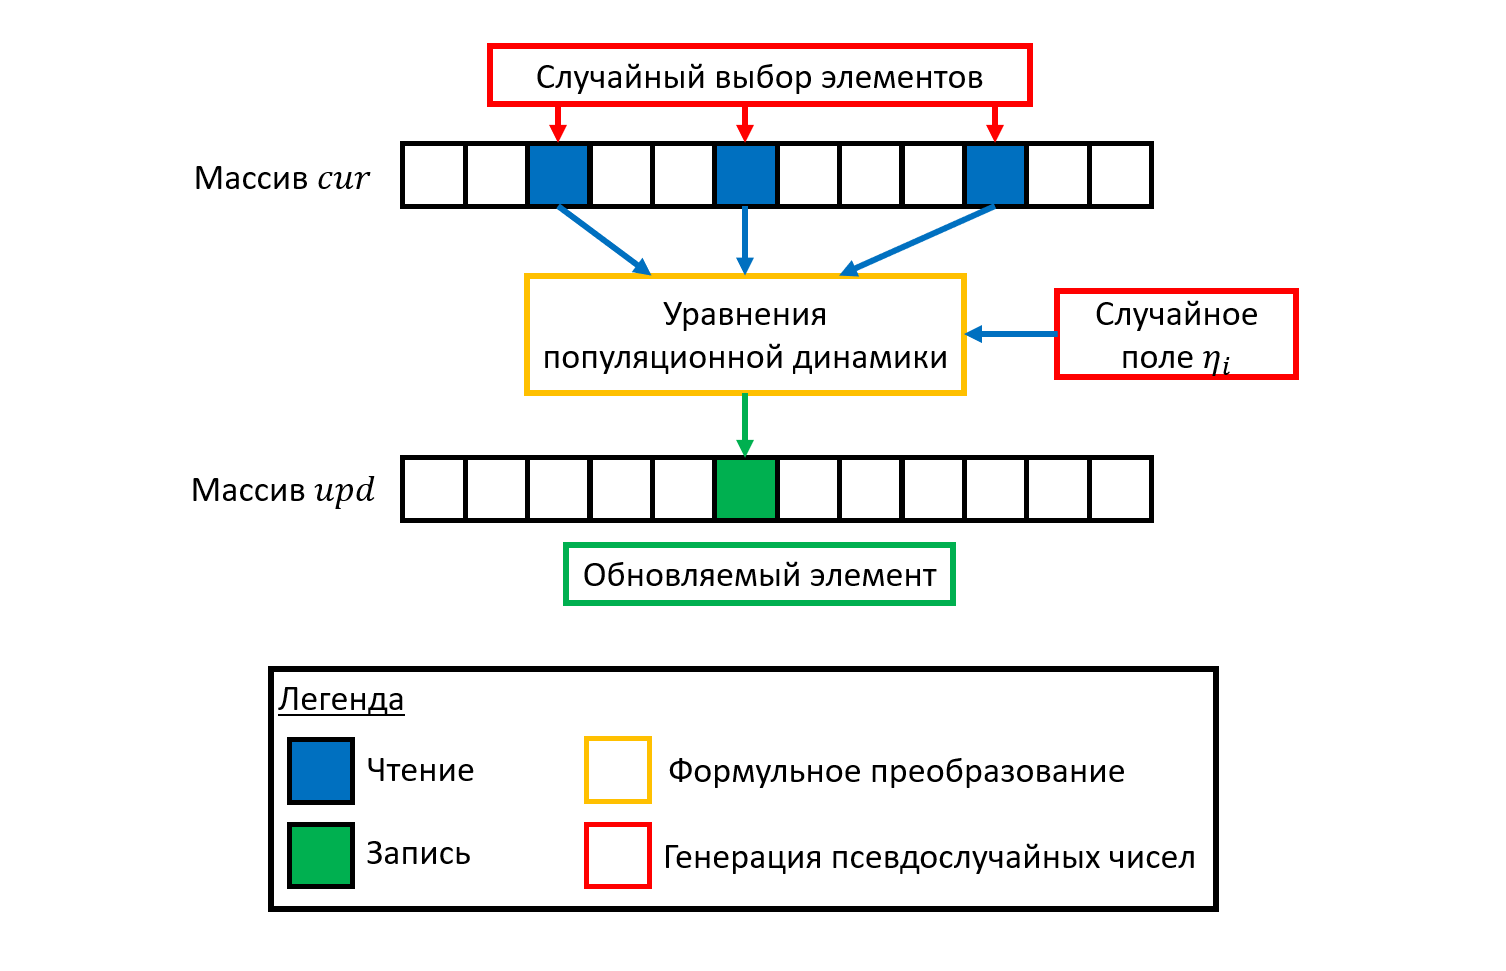
\includegraphics[width=0.8\textwidth]{Convetional_population_dynamics_scheme.png}
	\caption{Принципиальная схема одного шага алгоритма популяционной динамики.}
\end{figure}

\subsubsection{Вопросы сходимости алгоритма}
У алгоритма есть два набора параметров:
\begin{enumerate}
	\item внешние параметры (физические): $\Delta$, $g$, $K$
	\item Внутренние параметры алгоритма: размеры массивов $M$, число итераций $N$, значение параметра уширения уровней $\gamma$. 
\end{enumerate}
Как уже обсуждалось ранее в теоретическом описании алгоритма, физическая ситуация соответствует взятию пределов в следующем порядке:
$$
\lim_{\gamma \rightarrow +0} \lim_{M \rightarrow \infty} \lim_{N \rightarrow \infty}
$$
так что величина $M$ имеют роль схожую с тем, которую в исходной задаче выполняло число узлов графа. Однако, на практике взятие этих пределов сводится к надежде, что начиная с некоторого момента получаемые распределения перестают видимым образом зависеть от этих внутренних параметров. Иными словами, эти пределы берутся только численно, так что полная процедура сводится к следующему
\begin{enumerate}
	\item При фиксированных $\gamma, M$ провести достаточное большое число итераций алгоритм $N^*$, чтобы эмпирическое распределение $P[\gamma, M ,N](G_{i \rightarrow j})$ перестало видимым образом изменяться. Это можно фиксировать, например, по динамике моментов распределения (которые легко поддерживать), а также различными статистическими критериями, вроде Критерия Колмогорова-Смирнова. Оценка на минимальное число необходимых итераций имеет вид $N^{*} \gtrsim \frac{\ln M}{\ln K}$.
	\item Далее, при заданном $\gamma$ ровно тем же способом находится значение $M^*$, после которого распределение $P[\gamma, M, N^*(\gamma, M)]$ перестаёт изменяться. Трудности состоят в том, что оценка на необходимую величину размера выборки в случае делокализованной фазы является очень быстро растущей с уменьшением $\gamma$: $\ln M^{*} \gtrsim \ln K \ln \frac{1}{\gamma}$. 
	Отметим, что полученная оценка получается очень быстро растущей с $\gamma$, что в общем случае усложняет интерпретацию результатов, требуя тщательного анализа данных на предмет насыщения по данным пределам.
	\item Наконец, точно также подбирается параметр $\gamma^*$, характеризующий сходимость численного приближения к истинному распределению $$P\left[ \gamma^*, M^*(\gamma^*), N^*\left( \gamma^*, M^{*}(\gamma^*) \right) \right]$$. Отметим, однако, что для некоторых величин зависимость от регуляризации $\gamma$ будет присутствовать на любых масштабах. В таких случаях требуется изучать факт выхода этих зависимостей на их асимптотическую форму. Примером является величина IPR \eqref{eq:IPR_through_GF}: в зависимости от устройства состояний она будет вести себя или как $L \propto \gamma$ (делокализованная фаза) или выходить на некоторое постоянное значение (соответствует локализации). Разумеется, трудность представляет установления того или иного поведения при анализе данных численного счёта. Далее мы проиллюстрируем практический критерий, по которому будем определять насыщение по данному параметру.
\end{enumerate}
Детали и тонкости практической реализации этой сходимости мы проиллюстрируем далее.  


\subsection{Оптимизация}
Автором данной работы также предлагается оптимизация описанного алгоритма, заключающаяся в том, чтобы не различать обновляемые и текущий массивы. Иными словами, в памяти держится только один массив, который служит и источником для случайного выбор элементов, и местом записи результата вычислений по уравнениям популяционной динамики \eqref{eq:Population_dynamics_final_equations}. Наглядным образом эта модификация представлена в виде схемы на Рис. \ref{fig:Optimized_PD_scheme}.
\begin{figure}[h]
	\label{fig:Optimized_PD_scheme}
	\centering
	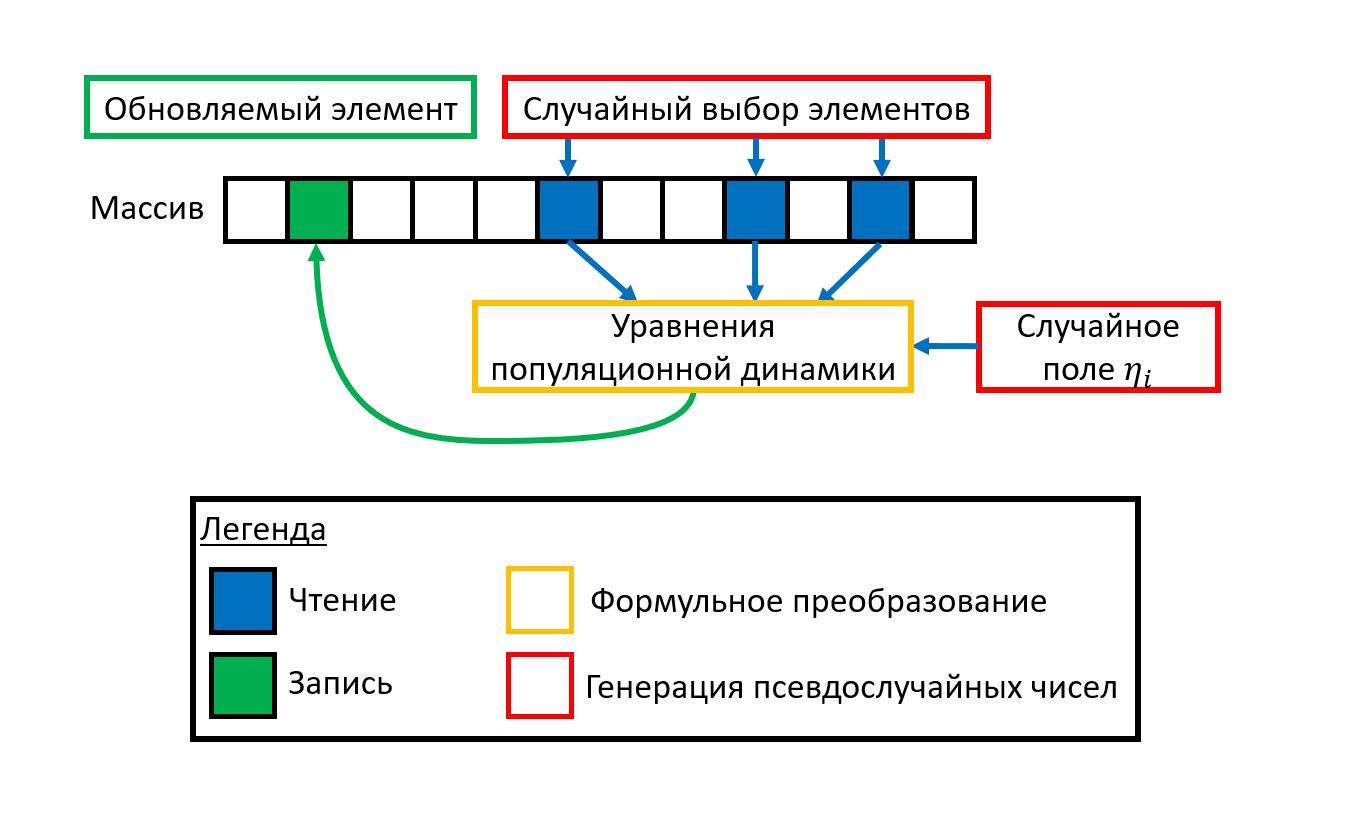
\includegraphics[width=0.8\textwidth]{Optimized_population_dynamics_scheme.png}
	\caption{Принципиальная схема одного шага оптимизированного алгоритма популяционной динамики. Следует сравнивать с Рис. \ref{fig:Population_dynamics_algorythm_scheme}: разница состоит в объединении ролей массивов $cur$ и $upd$}
\end{figure} 

Целями этой оптимизации является
\begin{itemize}
	\item очевидная экономия памяти, которая необходима для достижения упомянутой сходимости по размеру выборки $M$, так как характерные значения $M \sim 10^8$ лежат на границе доступных для вычислений ресурсов
	\item Гораздо менее очевидная оптимизация по количеству необходимого для сходимости количества итераций $N$. Строгих доводов о том, почему оптимизированный вариант алгоритма должен работать быстрее, нету, однако качественно получаемое на практике ускорение можно объяснить тем, что при подходе к концу массива в рамках одной итерации массив уже эффективно содержит обновлённую выборку, поэтому при генерации нового значения элементы из конца массива будут с большей вероятностью воспроизводить результат работы на большем количестве итераций. Тем самым, за одну итерацию этот алгоритм эффективно совершает несколько итераций классического варианта.
\end{itemize} 

Отметим, тем не менее, что строго говоря, существует вопрос о степени правильности получаемый выборки, поскольку, как отмечено выше, конец массива эффективно претерпел большее число итераций, нежели его начало. Однако, поскольку мы занимаемся поиском \textit{стационарной точки} отображения \eqref{eq:Population_dynamics_final_equations}, то на поздних этапах распределение эффективно <<забывает>> количество сделанных итераций, а потому результаты работы обоих алгоритмов (классического и оптимизированного) идентичны. Разумеется, данные рассуждения являются сугубо качественными, и серьёзным аргументом будет лишь практическая проверка степени схожести ответов для двух версий алгоритма.



\section{Тестирование и интерпретация особенностей работы алгоритма}
В этом разделе будут обсуждены основные практические аспекты применения описанного выше алгоритма популяционной динамики. При обсуждении рассматриваться будет только поведение локальной плотности состояний, как более наглядной величины для демонстрации ключевых особенностей.

\subsection{Эффективность использованных оптимизаций}
Прежде всего, проверим, является ли предложенная оптимизированная версия алгоритма рабочей. Критерием идентичности алгоритмов служит идентичность распределений плотности после выхода в стационарный режим. Детали проверки следующие:
\begin{itemize}
	\item на каждой итерации записывалась полная выборка, из которой потом вычислялись все нужные характеристики распределения.
	\item Параметры симуляций выбирались так, чтобы наблюдалось наиболее широкое распределение $\rho$, что даёт больше возможностей для явления потенциальных различий в алгоритмах. Численные значения следующие:
		\begin{itemize}
			\item Внешние физические параметры: $ K = 2, g = 0.15, \Delta = 2\exp \left\{ - \frac{1}{g} \right\}$
			\item Постоянные параметры алгоритма: $ \gamma = 10^{-7}, M = 2^{22} \approx 4.2 \cdot 10^6$
			\item Полное число итераций $N = 256$.
		\end{itemize}
	\item Стационарное значение оценивалось усреднением по большому числу итераций в области видимого постоянства значения. В данном случае, это диапазон  $N \in [60, 256]$.
\end{itemize}
Сравнение получающихся распределений приведено на Рис. \ref{fig:Methods_comparison_stationary_distribtution}, а демонстрация скорости сходимости на примере первых моментов приведена на Рис. \ref{fig:Methods_comparison_moments_convergence}.
\begin{figure}[h]
	\label{fig:Methods_comparison_stationary_distribtution}
	\centering
	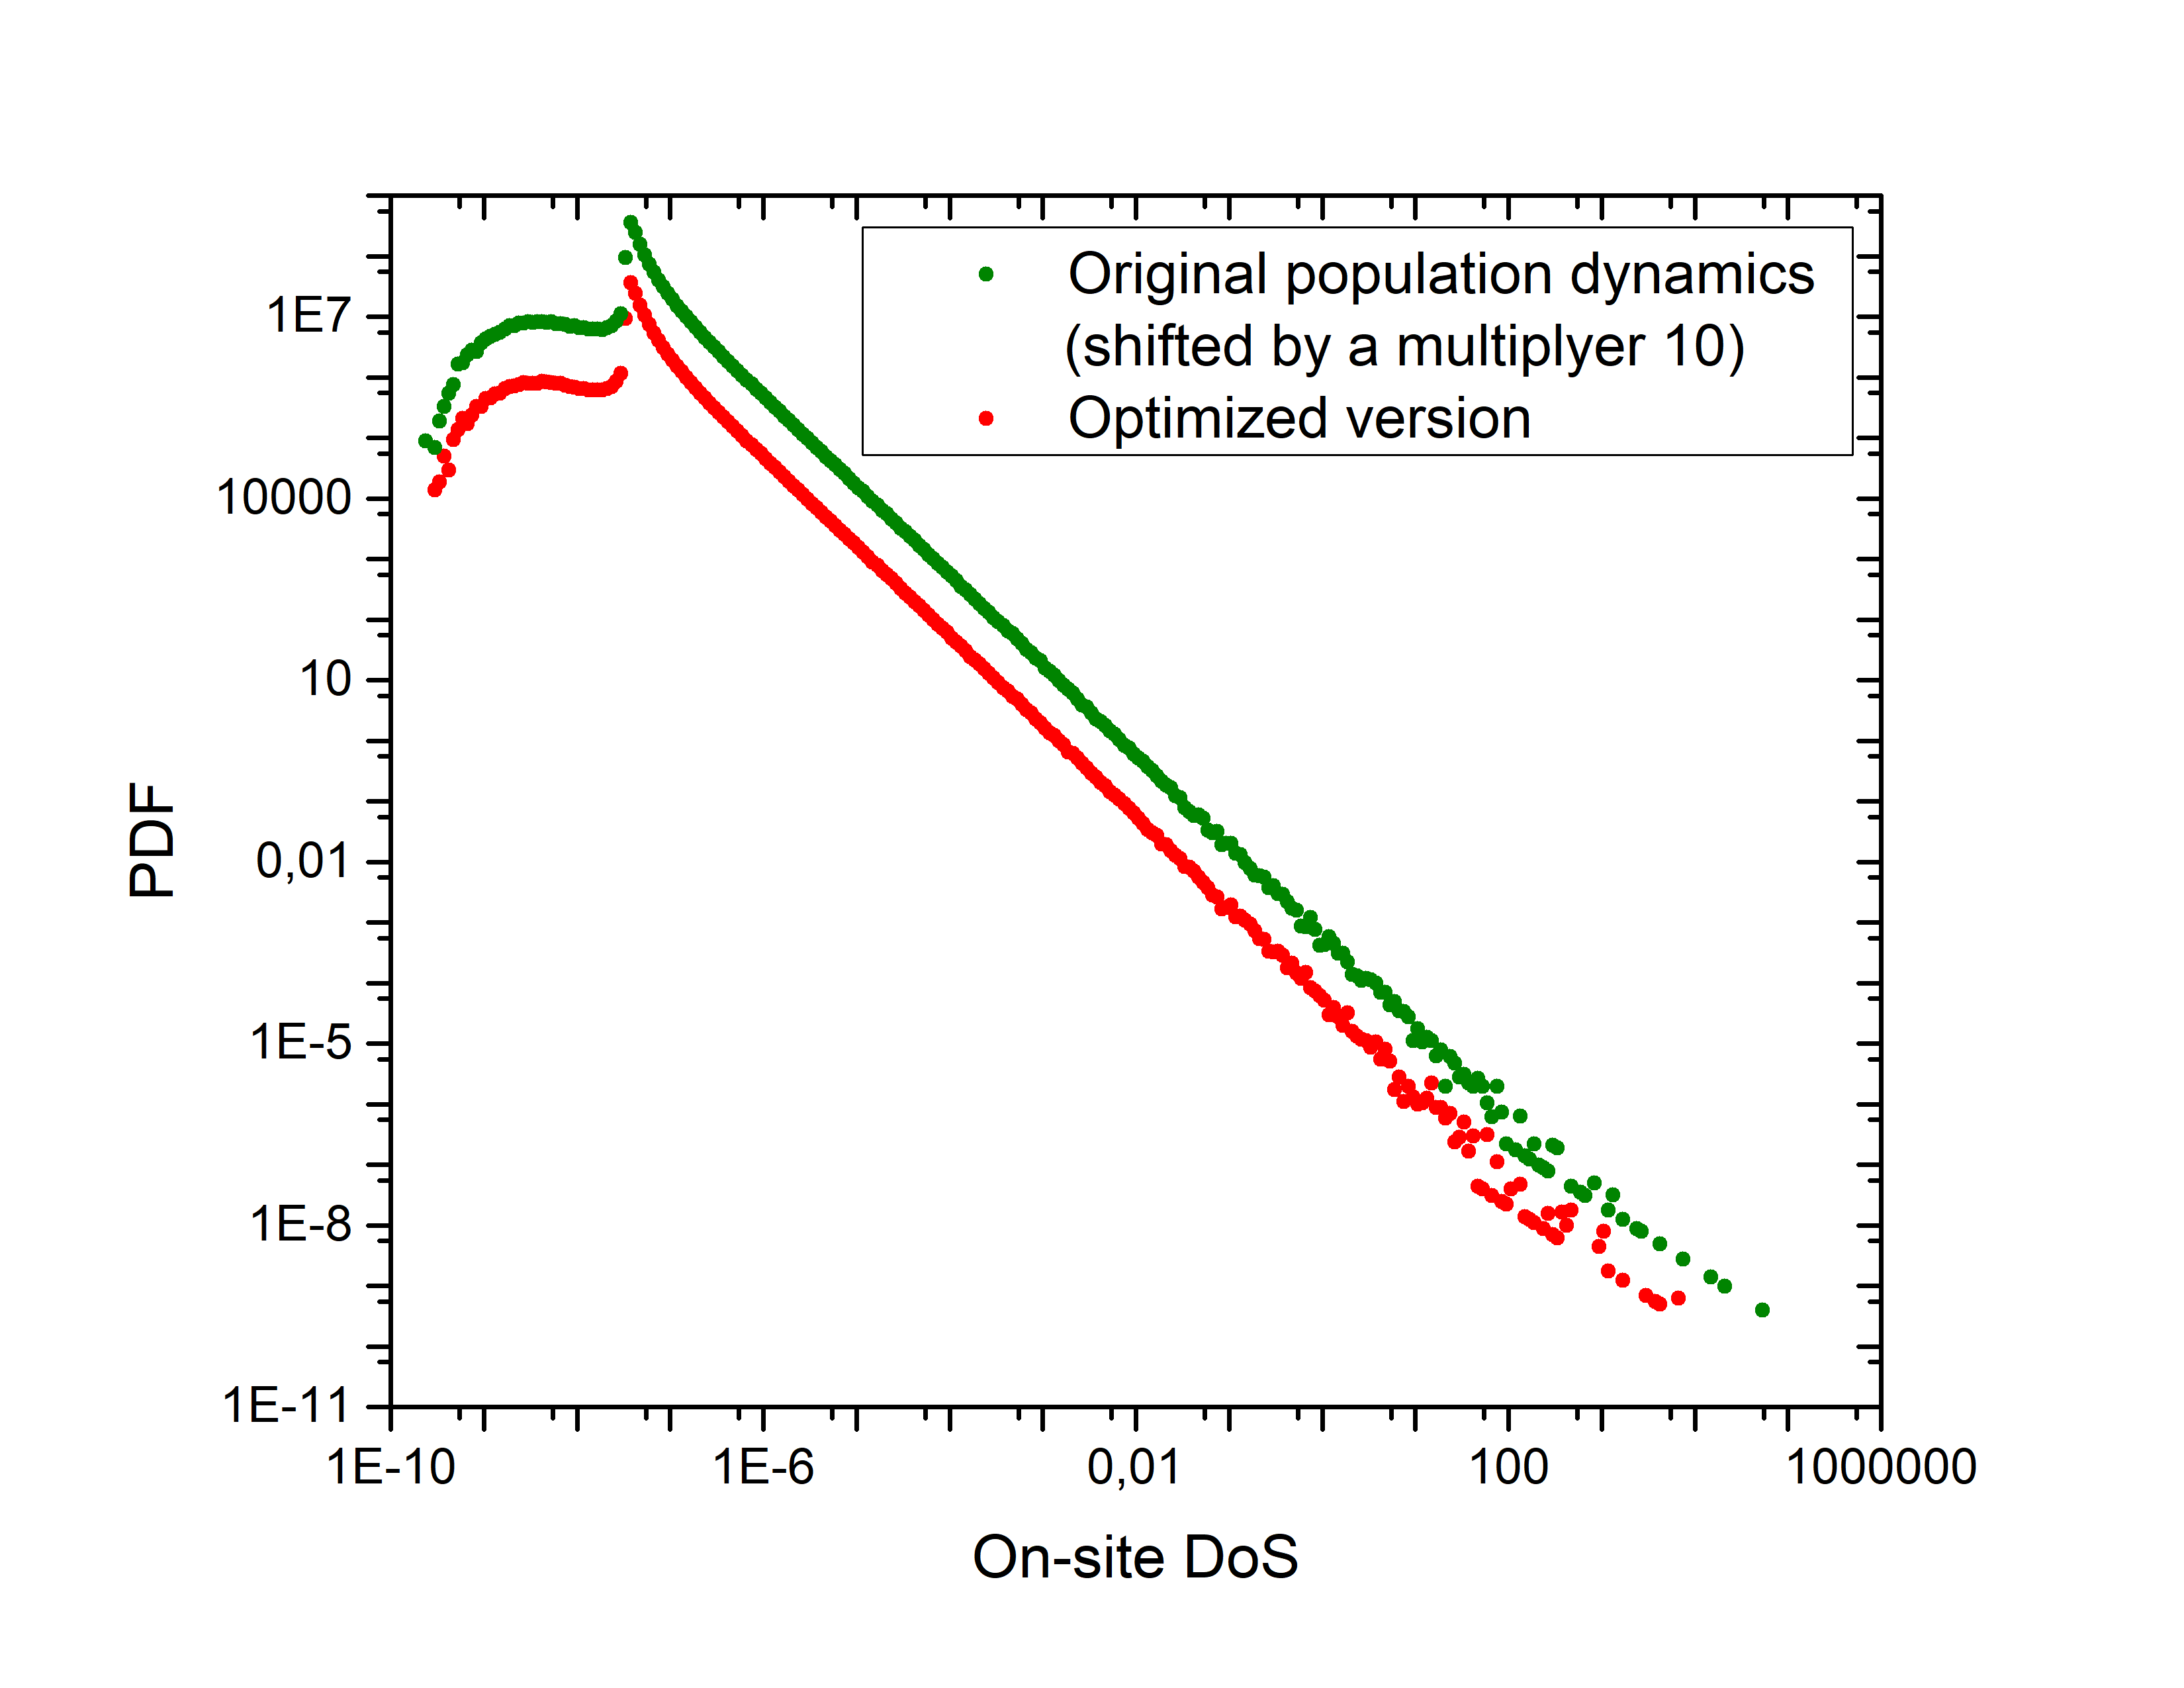
\includegraphics[width=0.8\textwidth]{Algo_comp_versions_distr.png}
	\caption{Стационарное ($N = 128$) эмпирическое распределение плотности для обеих версий, причём данные для наглядности сдвинуты постоянным множителем $10$, так как при наложении они совпадают (очевидно, постоянный множитель портит только нормированность распределения, но не его форму). Подробные технические данные симуляции см. в тексте.}
\end{figure}

\begin{figure}[h!]
	\label{fig:Methods_comparison_moments_convergence}
	\centering
	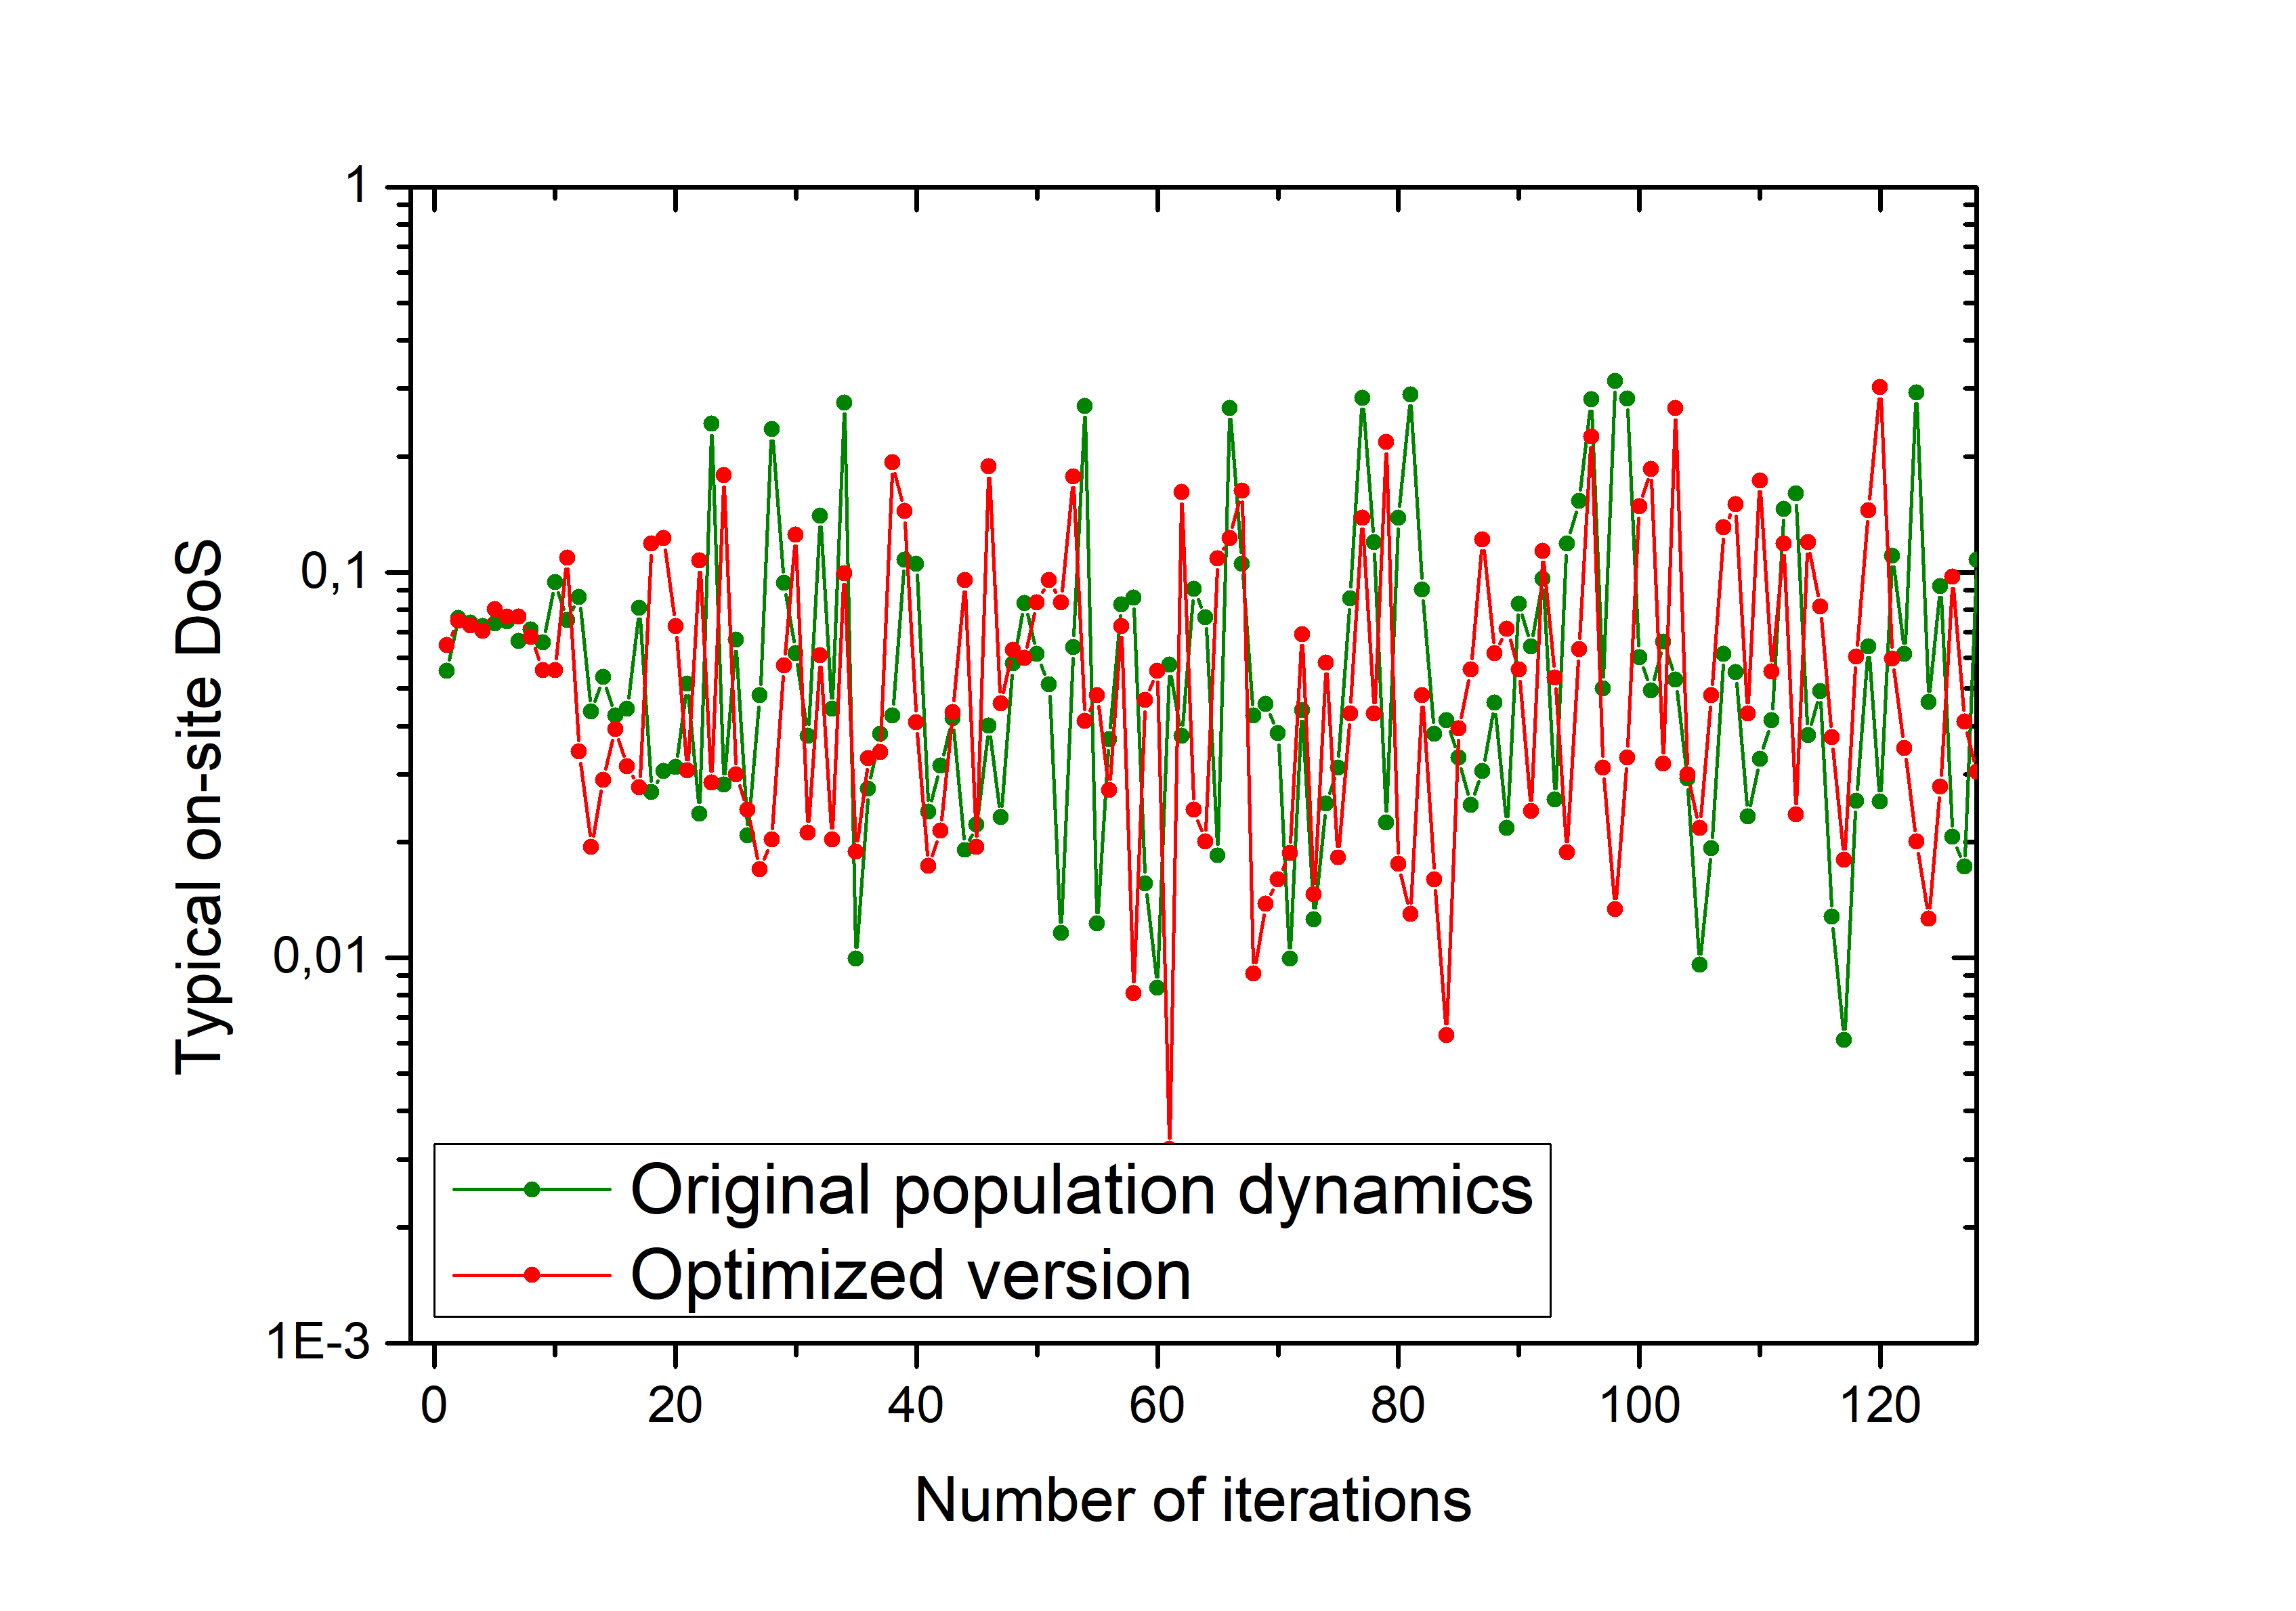
\includegraphics[width=0.49\textwidth]{Algo_comp_versions_mean.png}
	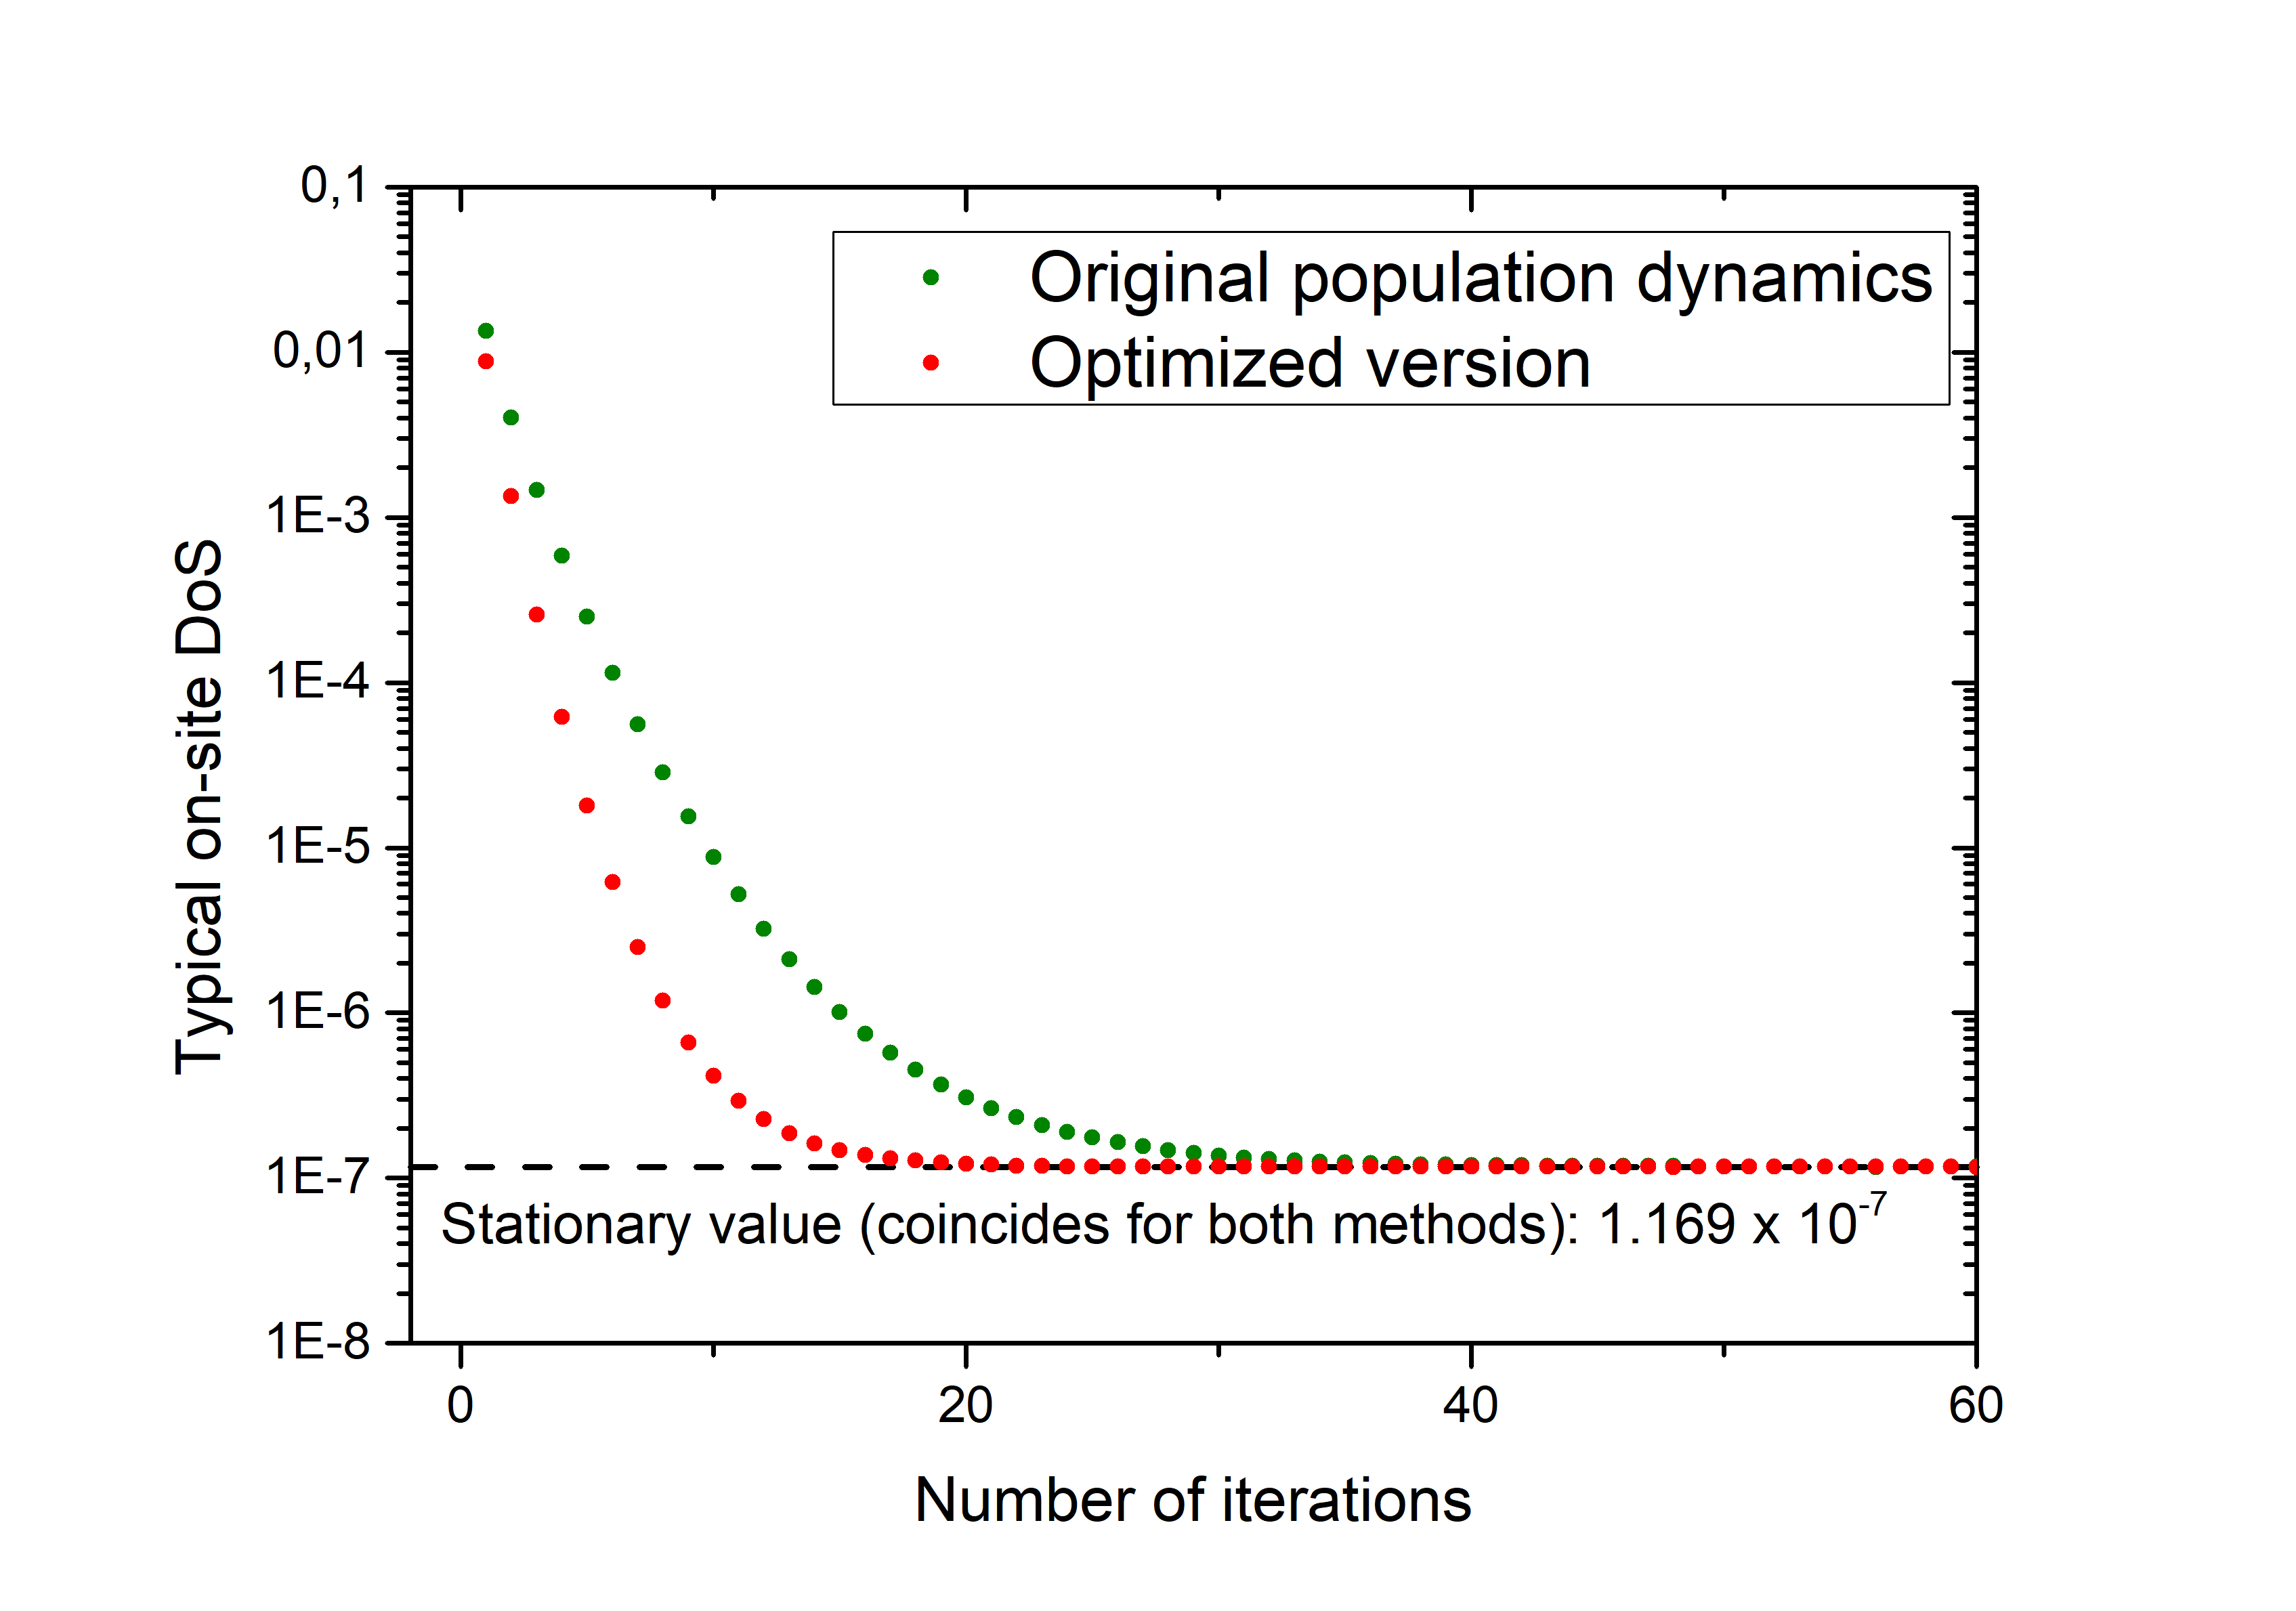
\includegraphics[width=0.49\textwidth]{Algo_comp_versions_typical.png}
	\caption{Слева: зависимость средней плотности состояний $\langle \rho \rangle$ от числа итераций для обеих версий. Справа: зависимость типичной плотности состояний $\exp{\langle \ln \rho \rangle}$ от числа итераций для обеих версий. Подробные технические данные симуляции см. в тексте.}
\end{figure}

Обзор специфики формы распределения см. в \autoref{Result}, а на данный момент основные выводы по данным следующие:
\begin{itemize}
	\item как наглядно видно из Рис. \ref{fig:Methods_comparison_stationary_distribtution}, алгоритмы дают абсолютно идентичные результаты, так как формы графиков полностью одинаковые, а при наложении они тождественно совпадают.
	\item Как показывают данные для зависимости типичной плотности состояний от числа итераций на Рис. \ref{fig:Methods_comparison_moments_convergence} слева, оптимизированная версия работает примерно в два раза быстрее, что для неигрушечных симуляций сэкономило автору работы недели компьютерного времени.
	\item Данные по средней плотности состояний на Рис. \ref{fig:Methods_comparison_moments_convergence} справа говорят о том, что оба метода в одинаковой степени чувствительны к статистическим флуктуациям, обусловленным конечным размером выборки (об этом подробнее см. далее).
\end{itemize}
Как итог, можно утверждать, что оптимизация явно имеет ощутимый смысл.


\subsection{Сравнение с точной диагонализацией}
Для проверки общей валидности применяемого метода предлагается сравнить его с процедурой \textit{точной диагонализации}, гарантированно воспроизводящей правильное распределение плотности состояний для конечных системы. Суть этой процедуры кратко описывается следующим образом:
\begin{enumerate}
	\item генерируется случайный $K$-регулярный граф некоторого размера $M \sim 10^3$.
	\item Генерируется случайный набор полей $\eta_i$, и по определению \eqref{eq:Local_operator_definition} составляется матрица $C$. 
	\item Применяется численный алгоритм <<FEAST>> поиска всех собственных векторов матрицы с собственным числом, лежащим в конечной малой окрестности $\delta E$ требуемого собственного числа ($1$ в нашем случае).
	\item Локальная плотность состояний на каждом узле оценивается по формуле
	$$
	\rho_i = \frac{1}{\delta E} \sum_k \left| \left\langle \psi_k | i \right\rangle \right|^2
	$$
	где $\psi_k$ -- найденные вектора, $i$ -- номер узла.
	\item По значениям найденных плотностей в нескольких реализациях беспорядка составляется выборка.
\end{enumerate}

\begin{figure}[h!]
	\label{fig:Exact_digonalization_different_matrix_sizes}
	\centering
	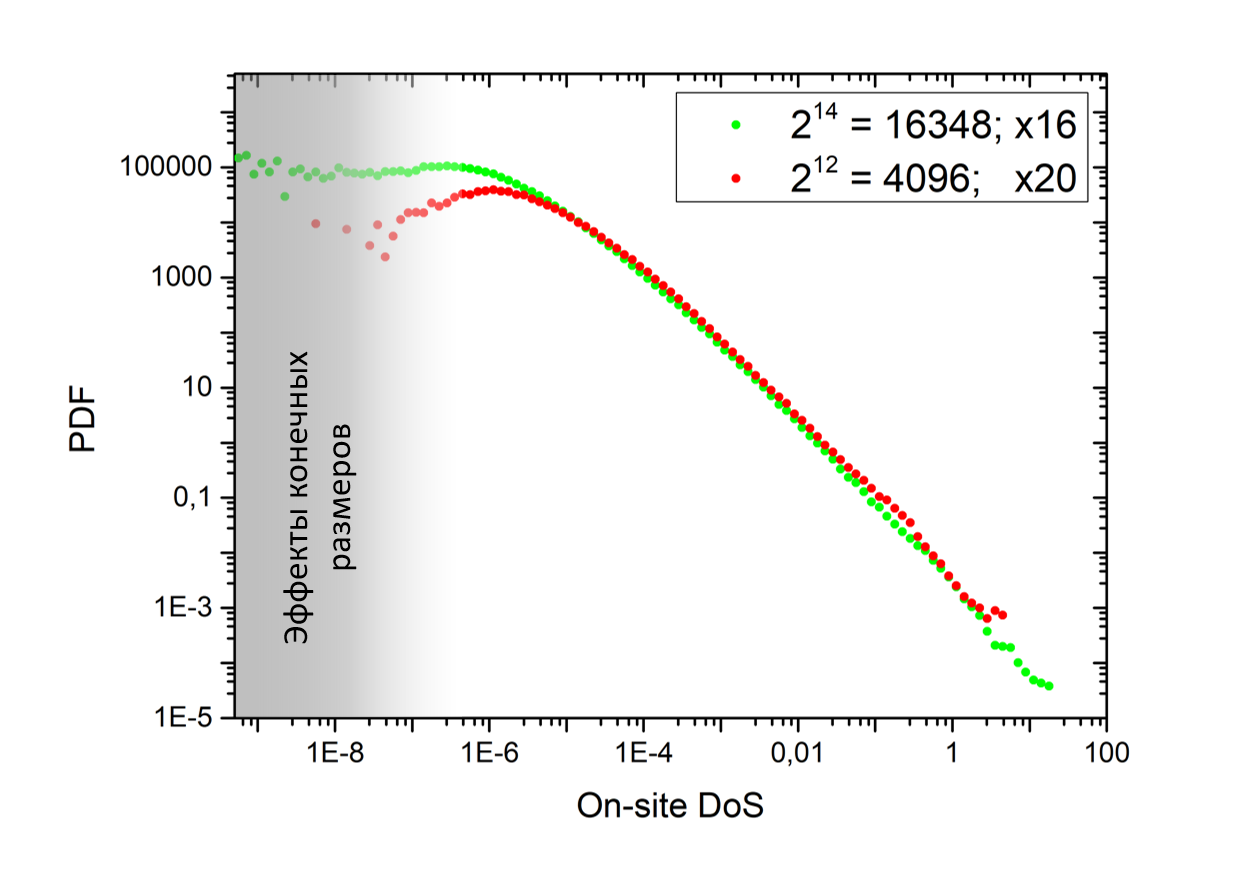
\includegraphics[width=0.8\textwidth]{ED_different_sizes_comp_distr.png}
	\caption{Эмпирическое распределение плотности состояний, полученное методом точной диагонализации для двух различных размеров матриц: 16 реализаций системы с $2^{14} = 16348$ узлами и 20 реализаций системы с $2^{12} = 4096$ узлами. Ширина окна по энергии $\delta E$ подстраивалась так, чтобы плотность состояний оценивалась по примерно одному и тому же количеству найденных состояний независимо от размера системы. Серым выделена область, в которой заметны существенные различия между данными из-за эффектов конечных размеров.}
\end{figure}

Особенности реализации и детали получения физически правильных результатов этой процедурой мы здесь обсуждать не будем. Продемонстрируем лишь тот факт, что полученная выборка, как и ожидается от такой этого метода, сильно чувствительна к размеру системы: данные для двух различных размеров матриц показаны на Рис. \ref{fig:Exact_digonalization_different_matrix_sizes}. Как видно из этих результатов, чтобы аккуратно исследовать термодинамический предел, необходимы гораздо большие размеры матриц, однако сложность $O(M^2)$ и такая же асимптотика для объёма занимаемой памяти делают этот метод малопригодным для наших целей.

\begin{figure}[h!]
	\label{fig:Comparison_PD_vs_ED}
	\centering
	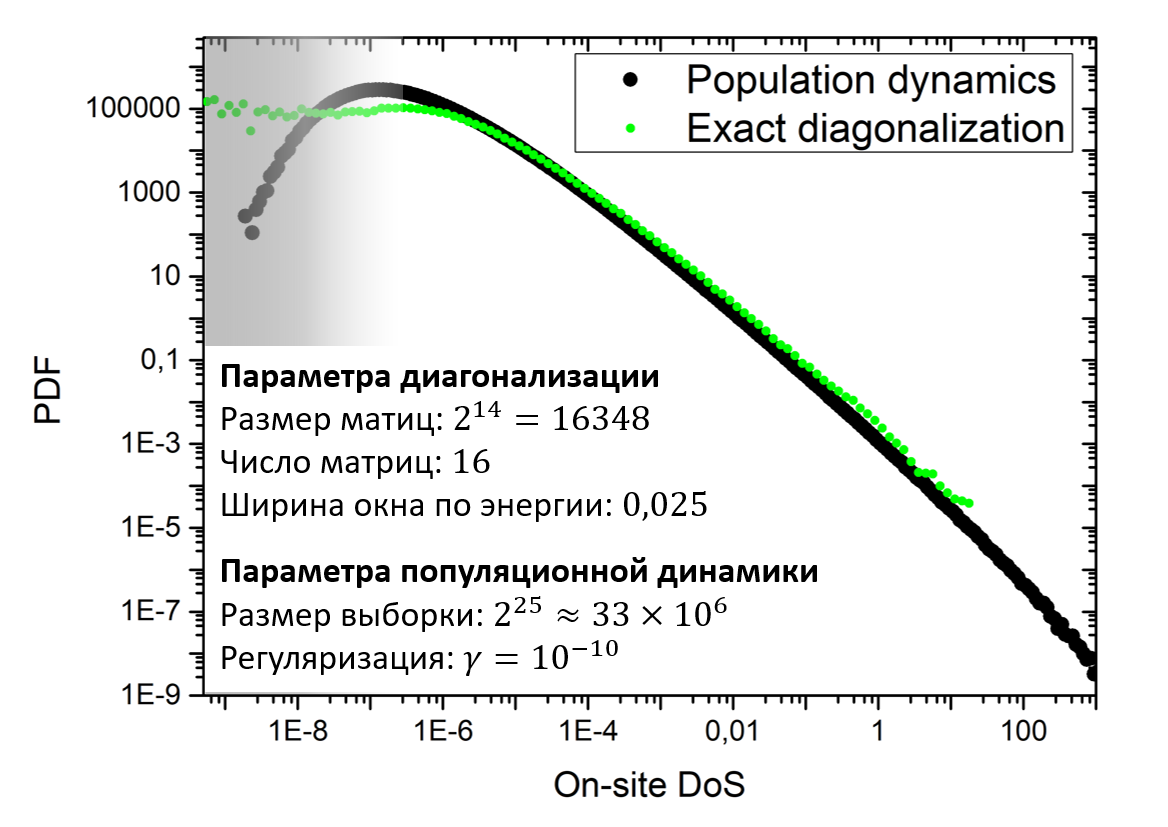
\includegraphics[width=0.8\textwidth]{Comparison_ED_vs_PD.png}
	\caption{Сравнение эмпирического распределения плотности состояний, полученных методами популяционной динамики и точной диагонализации. Значения внутренних параметров каждого из алгоритмов подписаны на рисунке. Серым отмечена область, не являющаяся достоверной для алгоритма точной диагонализации из-за эффектов конечных размеров.}
\end{figure}

Сравним данный <<эталонный>> метод с методом популяционной динамики. Результаты симуляции показаны на Рис. \ref{fig:Comparison_PD_vs_ED}. Значения физических параметров следующие: $ K = 10, g = 0.15 , \Delta = 2 \exp\left\{ -\frac{1}{g} \right\}$. Значения внутренних параметров обоих алгоритмов также указаны на Рис. \ref{fig:Comparison_PD_vs_ED}

Как следует из результатов, наш метод показывает себя полностью состоятельным, а также способным разрешить меньшие значения плотности состояний, реализуемые только в очень больших системах, недоступных для метода точной диагонализации. Отметим также, что авторами было проведено исследование поведения IPR, также идентичное в обоих методах.


\subsection{Особенности поведения численной процедуры при различных внутренних параметрах алгоритма}
В данном разделе мы опишем влияние внутренних параметров алгоритма популяционной динамки на результат его работы, прокомментируем возможные нефизические ситуации, и опишем общие идеи интерпретации данных, получаемых описанной численной процедурой. Существенно, речь далее будет идти о свойствах делокализованных состояний, так как все имеющиеся в распоряжении автора данные демонстрируют только такое поведение. Перечисленные ниже особенности не являются чем-то новым, однако их надо держать в уме при интерпретации данных. Их основной список следующий:
\begin{itemize}
	\item Динамические особенности поведения при итерировании алгоритма:
	\begin{itemize}
		\item хорошо определённое число итераций $N^{*}$, необходимое для установления распределения;
		\item зависимость $N^{*}$ от остальных внутренних параметров алгоритма $M, \gamma$;
		\item сильные флуктуации первых моментов распределения от итерации к итерации даже в стационарном режиме;
		\item хорошо определённое, слабо флуктуирующее значение типичного.
	\end{itemize}
	\item Особенности стационарного поведения:
	\begin{itemize}
		\item плохая статистика на верхней и нижней границах распределения при малых размерах выборки;
		\item резкая отсечка, пропорциональная $\gamma$, на нижней границе при недостаточно малых $\gamma$.
		\item В режиме насыщения плотности состояний по $\gamma$ величина IPR практически линейно зависит от $\gamma$, что соответствует физическому поведению $\lim_{\gamma \rightarrow +0} = 0$ и, соответственно, делокализованной фазе.
	\end{itemize}
\end{itemize}

Далее мы продемонстрируем наиболее информативные из указанных особенностей. С учётом вышесказанного, итоговая последовательность действий для корректного применения алгоритма следующая:
\begin{itemize}
	\item при использовании метода необходимо отследить несколько значений типичной плотности состояний при различном числе итераций и убедиться, что они совпадают;
	\item далее, необходимо удостовериться в независимости получаемых ответов от величин $\gamma$, рассмотрев зависимость типичной плотности состояний и IPR от $\gamma$ при нескольких разных значениях $M$: одна из этих величин должна насыщаться некоторым значением, а вторая -- демонстрировать уверенное степенное поведение, и в зависимости от результата делается заключение о структуре состояний (локализация / делокализация) \cite{AAT}.
\end{itemize}

\subsubsection{Влияние внутренних параметров $M, \gamma$ на сходимость по числу итераций $N$}
Прежде всего, продемонстрируем, как зависят средняя и типичная плотность состояний от числа итераций алгоритма, и как на характеристики сходимости влияют оставшиеся два внутренних параметра алгоритма $M, \gamma$. В нашем анализе мы не будем подробно останавливаться на IPR, поскольку его поведение \textit{во всём исследованном диапазоне параметров одинаково}  и имеет вид линейного по $\gamma$ поведения, слабо чувствительного к прочим параметрам. На Рис. \ref{fig:Convergence_for_various_gamma} приведены зависимости средней $\langle \rho \rangle$ и типичной $\exp \langle \ln \rho \rangle$ плотности состояний для различных $\gamma$, а на Рис. \ref{fig:Mean_convergence_for_various_M} --- данные только для среднего с различными небольшими размерами выборки $M$ (вид зависимости для типичного недемонстративен). Фиксированные физические параметры следующие: $K = 2, g = 0.15, \Delta = 2 \exp \left\{ -\frac{1}{g} \right\}$.

\begin{figure}[h!p]
	\label{fig:Convergence_for_various_gamma}
	\centering
	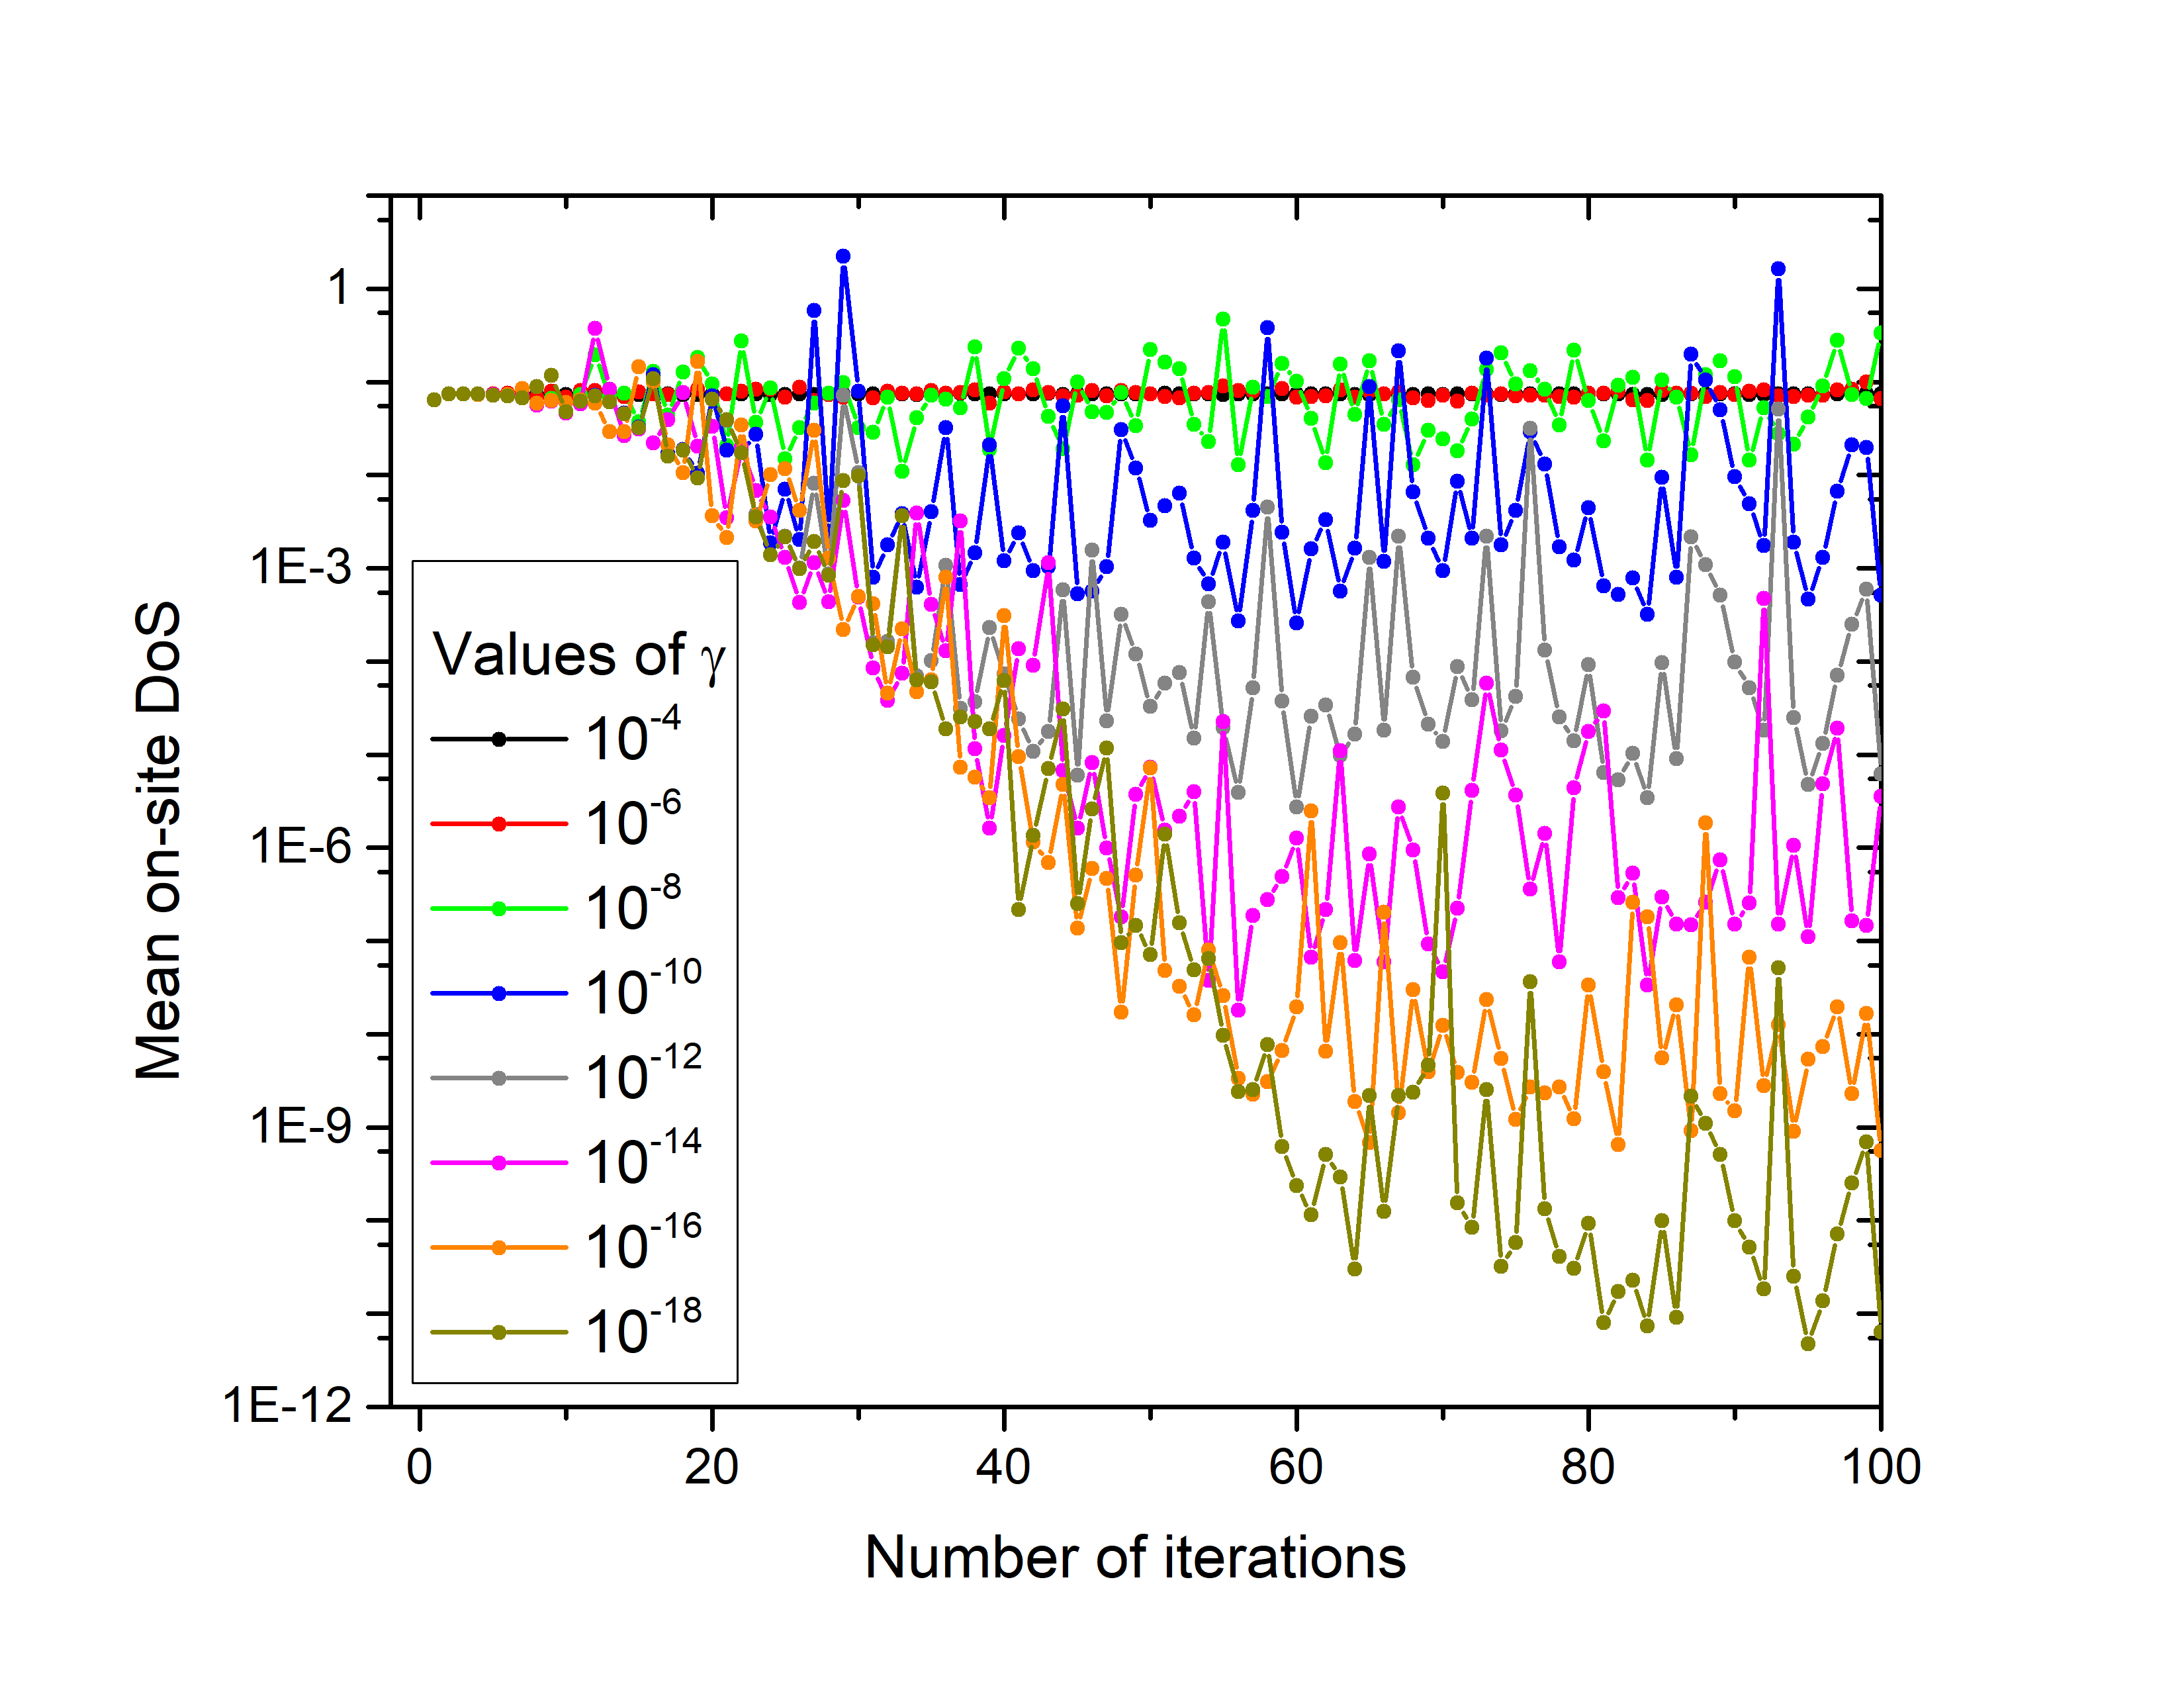
\includegraphics[width=0.85\textwidth]{Mean_convergence_various_gamma.png}
	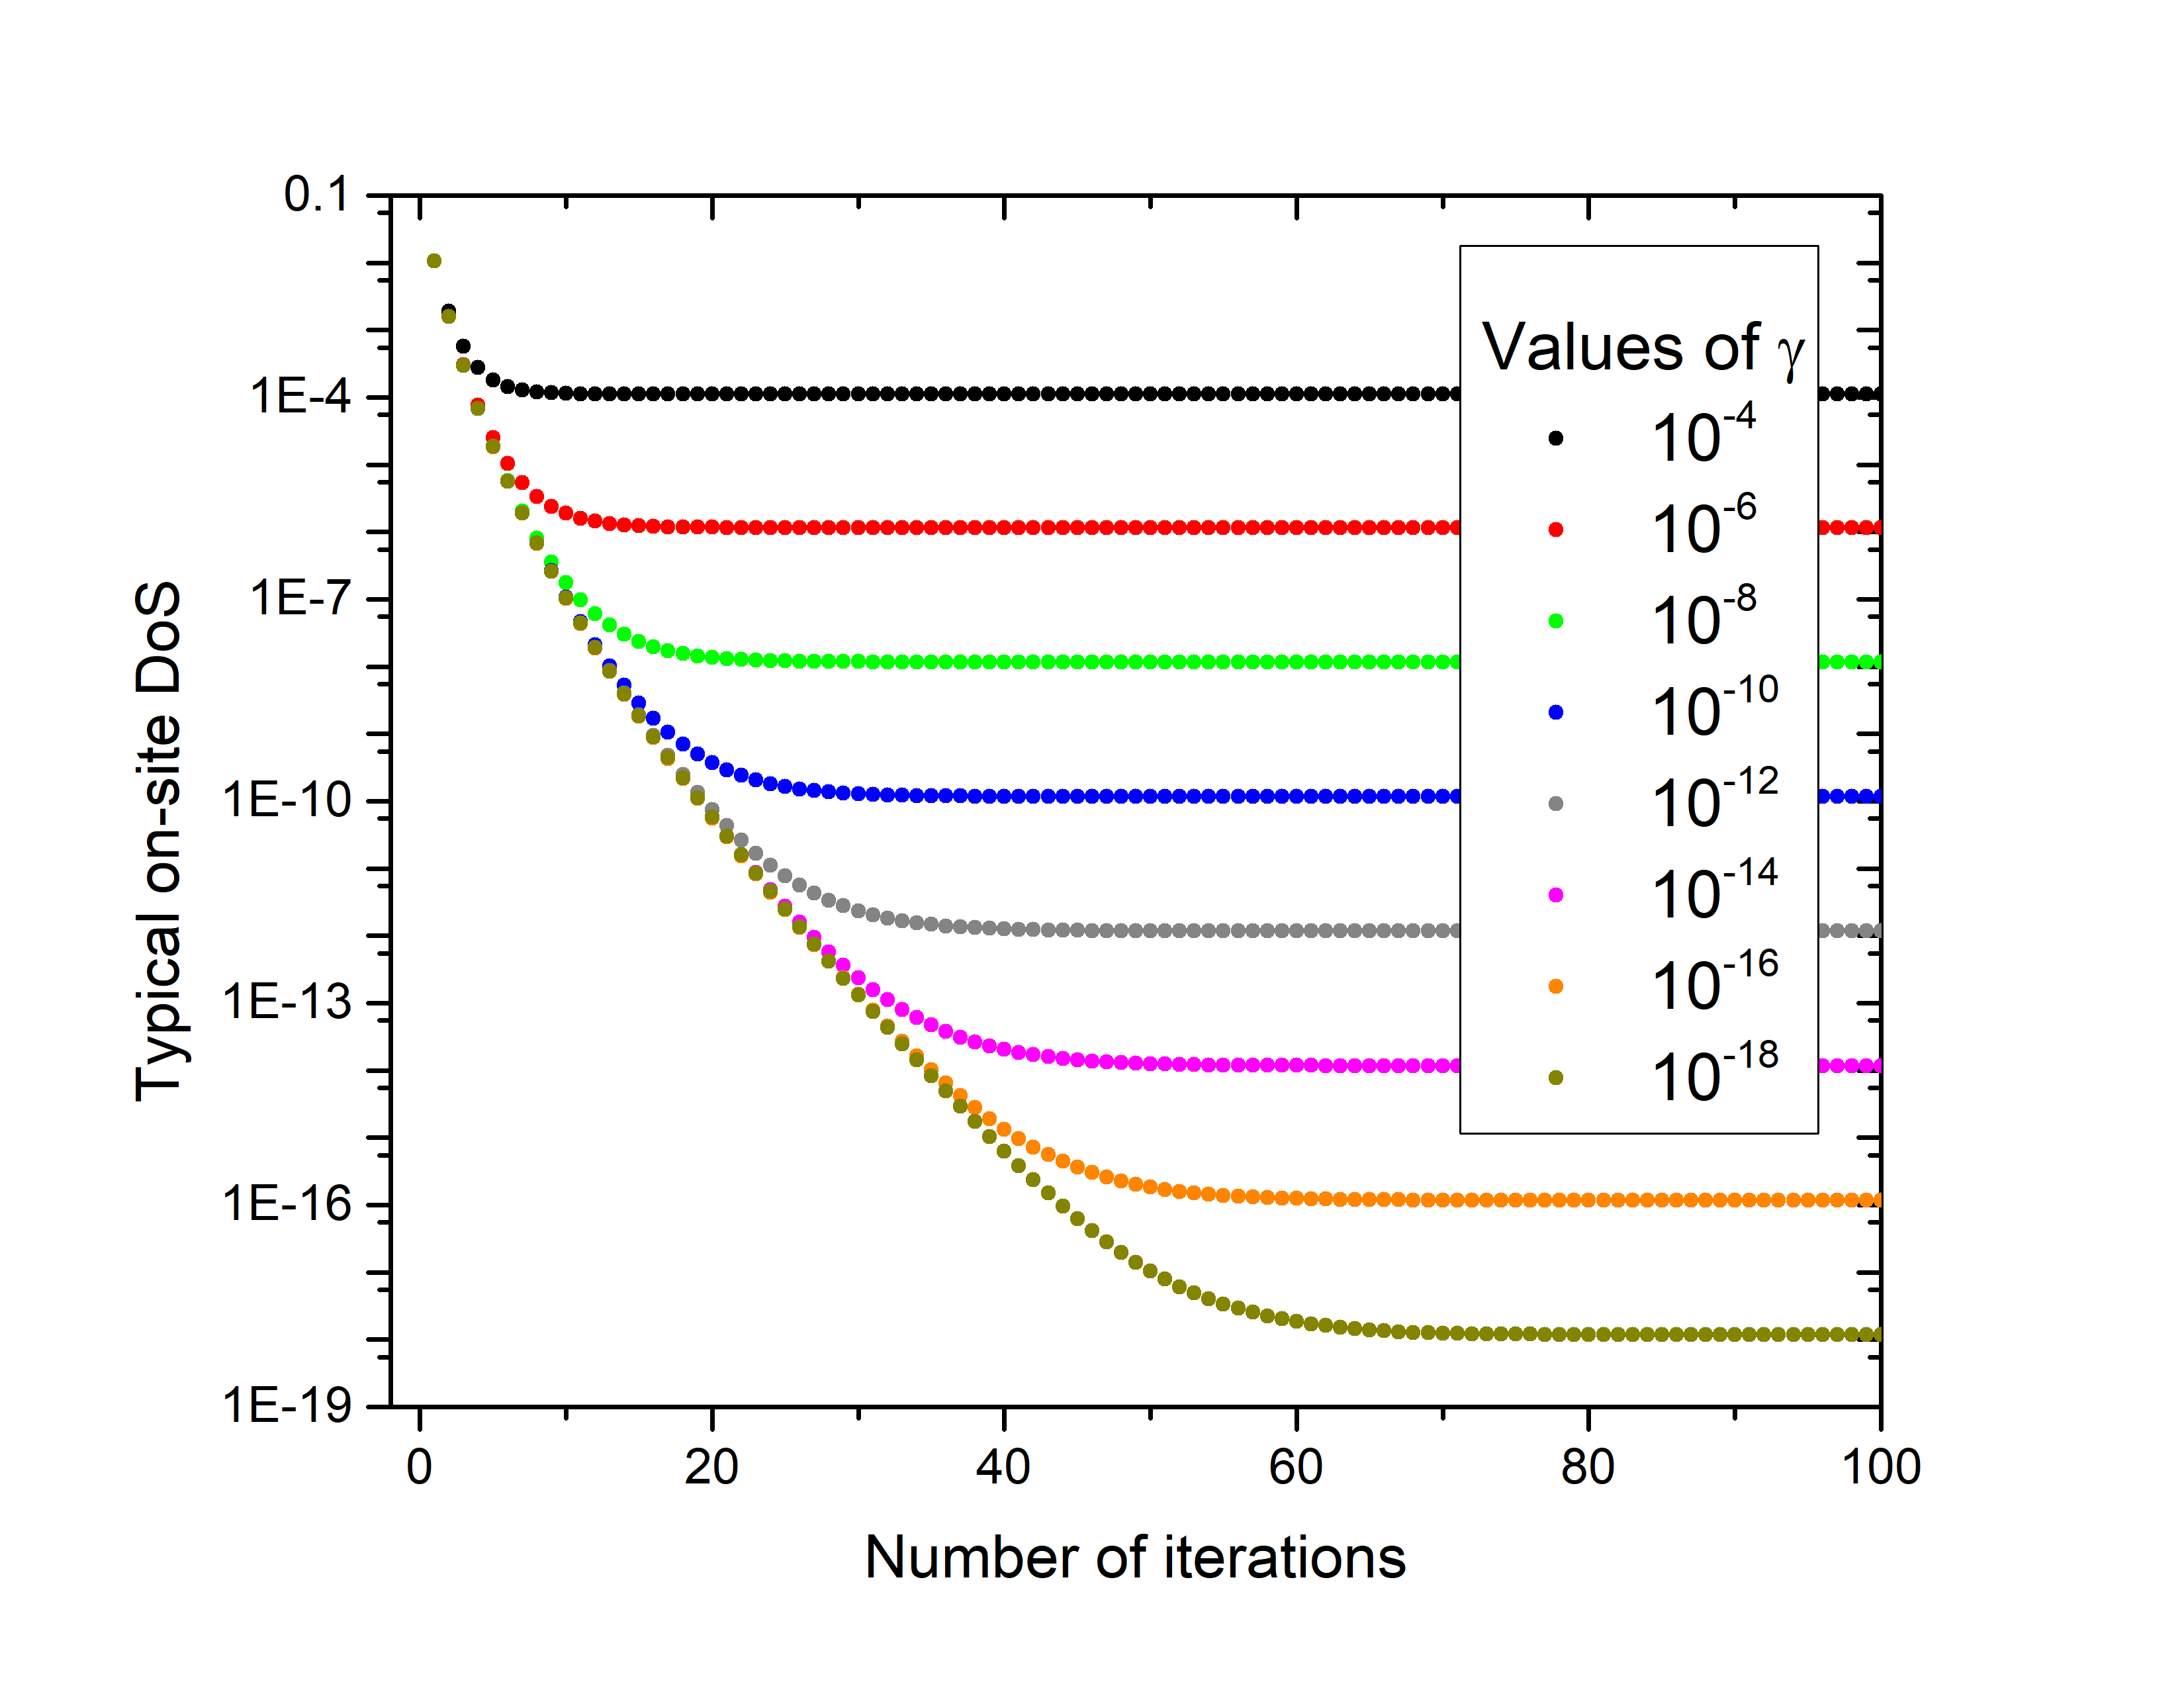
\includegraphics[width=0.85\textwidth]{Typical_convergence_various_gamma.png}
	\caption{Зависимость средней $\langle \rho \rangle$ (сверху) и типичной $\exp \langle \ln \rho \rangle$ (снизу) плотности состояний от числа итераций алгоритма при различных значениях $\gamma$. Размер выборки $M = 2^{26} \approx 6.7 \cdot 10^{8}$. Физические параметры симуляций см. в тексте.}
\end{figure}

\begin{figure}[h!p]
	\label{fig:Mean_convergence_for_various_M}
	\centering
	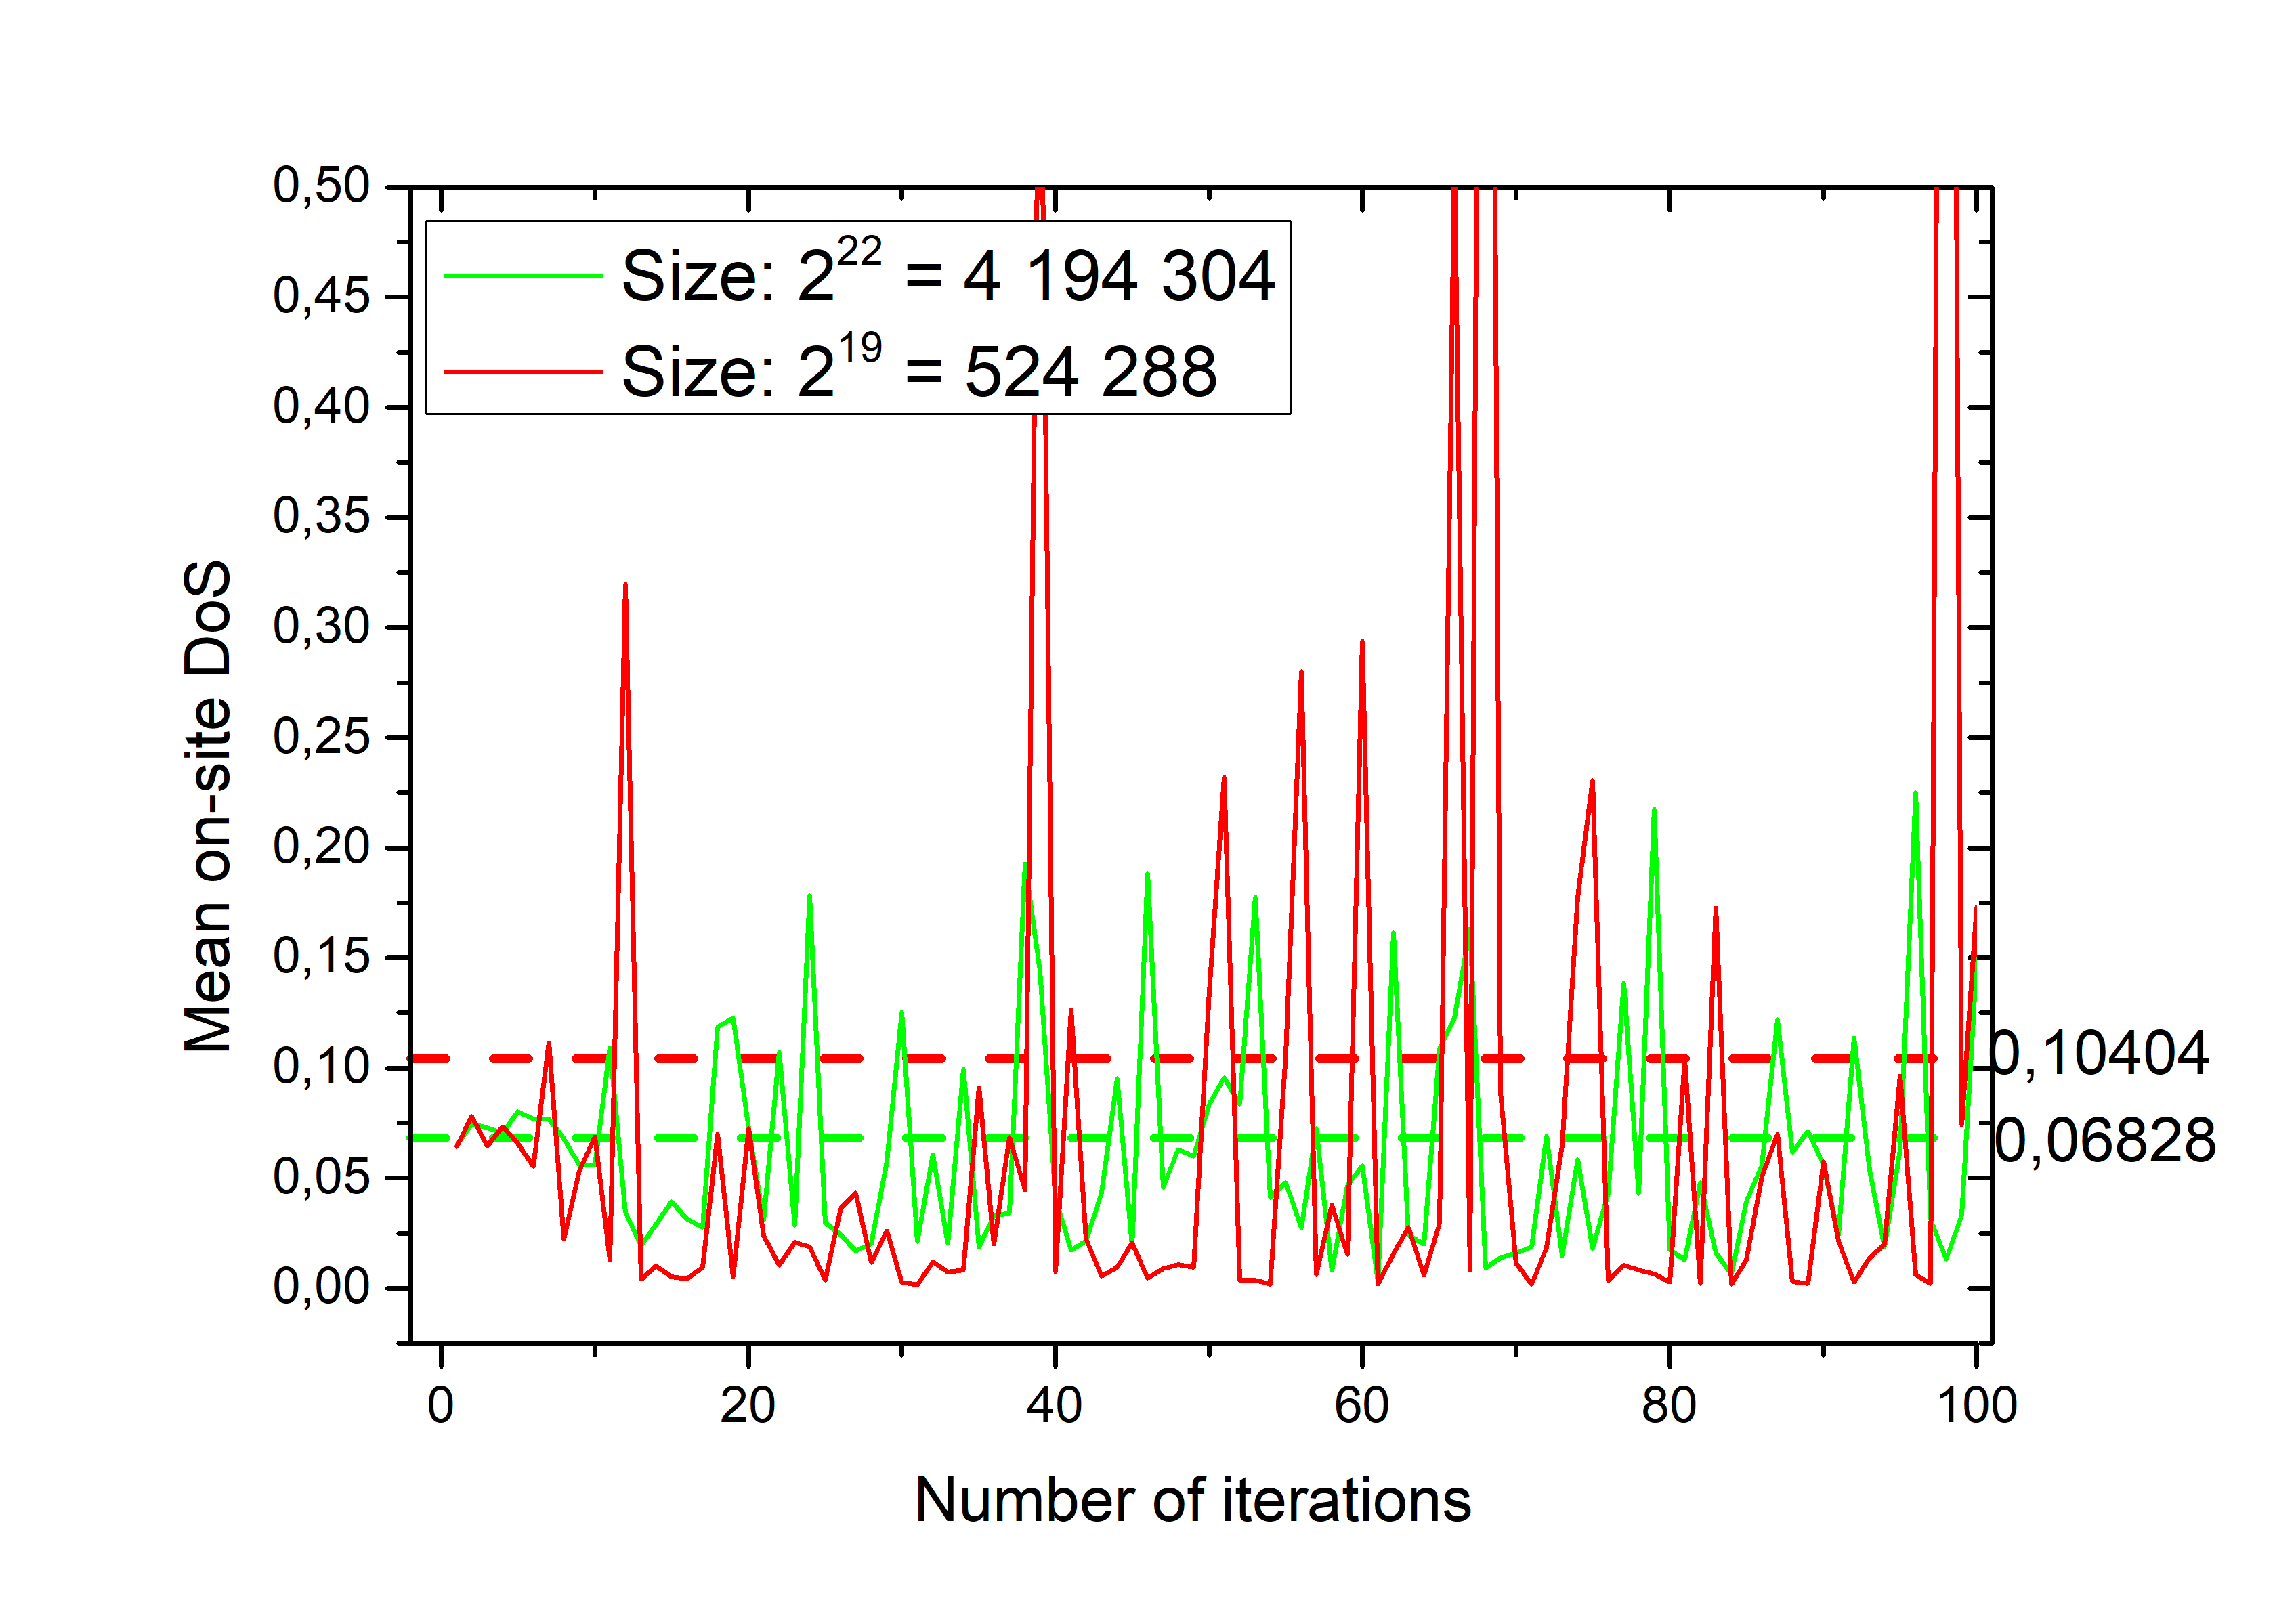
\includegraphics[width=0.8\textwidth]{Mean_convergence_for_various_M.png}
	\caption{Зависимость средней плотности состояний $\langle \rho \rangle$ от числа итераций алгоритма при двух различных значениях $M$ (указаны на рисунке). Значение регуляризации $\gamma = 10^{-7}$. Для сравнения на рисунке приведены также оценки для итерационного среднего вида $\overline{\langle \rho \rangle}$. Физические параметры симуляций см. в тексте.}
\end{figure}

Ключевые особенности приведённых зависимостей следующие:
\begin{itemize}
	\item имеется характерное время установления стационарного режима как для среднего, так и для типичного. Этот режим в неизменном виде наблюдается сколь угодно долго (в серии симуляций на Рис. \ref{fig:Convergence_for_various_gamma} максимальное число итераций составляет $N = 1000$).
	\item Факт совпадения времён установления среднего и типичного косвенно свидетельствует в пользу того, что данное время является характерным для установления всего распределения. Численные опыты с меньшим размером выборки (здесь не приведены) подтверждают это предположение.
	\item Время установления зависит от $\gamma$, причём зависимость на качественном уровне имеет степенной характер. Подробные исследования этой зависимости не проводились.
	\item В стационарном режиме среднее испытывает сильные флуктуации (в несколько порядков), амплитуда которых возрастает с уменьшением $\gamma$. На практике эти флуктуации означают, что среднее в этом алгоритме является плохо определённой величиной, поэтому для оценки первого момента распределения предлагается усреднять среднюю плотность состояний $\exp \overline{\ln \langle \rho \rangle}$ по итерациям.
	\item Значение среднего, около которого происходят флуктуации, и размах флуктуаций также сильно чувствительно к размеру выборки $M$. Более того, при малых размерах выборки стационарная динамика демонстрирует наличие резких пиков среднего, которые длятся ровно одну итерацию. Качественные комментарии, объясняющие это поведение, мы дадим чуть позже, когда разберёмся с влиянием параметров $\gamma, M$ на всё стационарное распределение.
	\item Напротив, типичное значение практически не испытывает флуктуаций и слабо чувствительно к размеру выборки, а потому является хорошо определённой характеристикой всего распределения. В купе с уже сказанным, это сильно облегчает задачу по выяснению степени сходимости алгоритма по числу итераций --- достаточно просто следить за установлением типичного (вместо того, чтобы хранить на каждой итерации всё распределение из $\sim 10^8$ значений). 
	\item Также важно заметить, что среднее и типичное являются сильно зависящими от $\gamma$. Это характерный признак отсутствия насыщения по $\gamma$. Поэтому в дальнейшем при предъявлении различного рода зависимостей будут приводиться версии этой зависимости при различных значениях $\gamma$, чтобы можно было судить о степени насыщения.
\end{itemize}

\subsubsection{Влияние параметров $M ,\gamma$  на форму стационарного распределения}
На Рис. \ref{fig:DOS_disribution_for_various_gamma} приведены формы стационарного распределения для двух различных значений $\gamma$, а на Рис. \ref{fig:DOS_disribution_for_various_M} --- для различных значений размера выборки $M$. Постоянные физические параметры всё те же: $K = 2, g = 0.15, \Delta = 2 \exp \left\{ -\frac{1}{g} \right\}$.
 
\begin{figure}[h!]
	\label{fig:DOS_disribution_for_various_gamma}
	\centering
	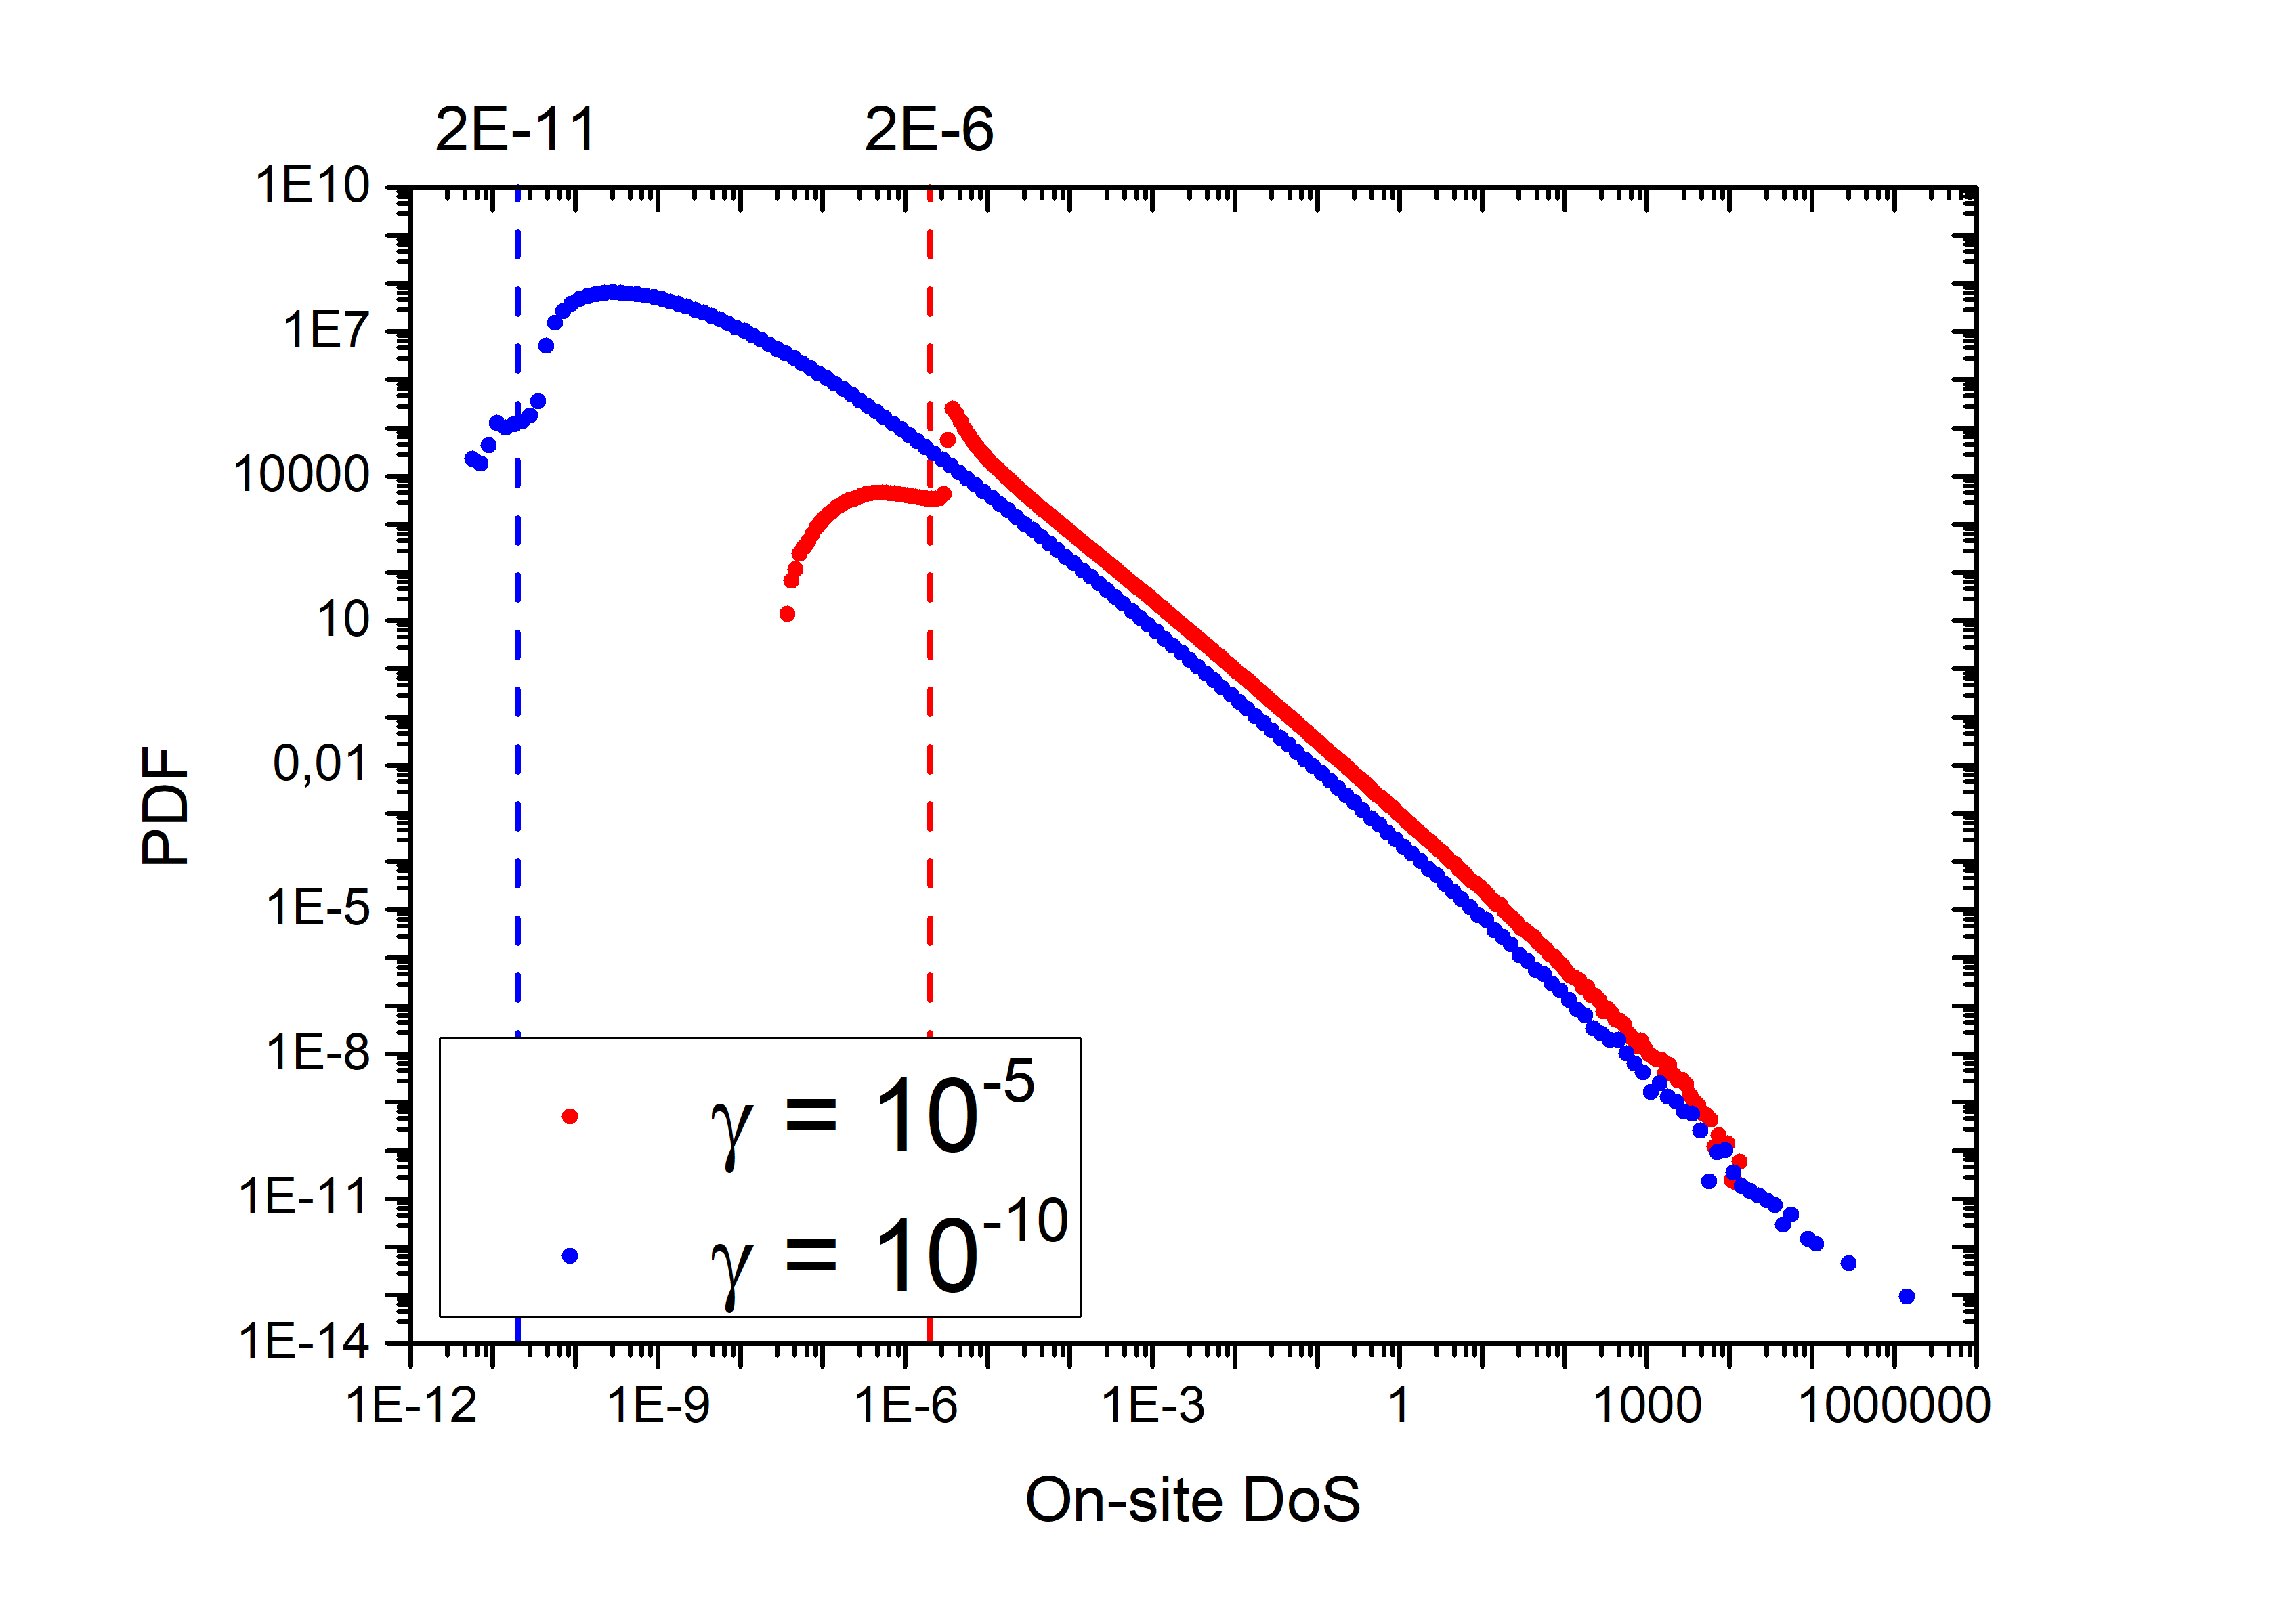
\includegraphics[width=0.8\textwidth]{DOS_disribution_for_various_gamma.png}
	\caption{Форма стационарного распределения при двух различных значениях параметра $\gamma$ (указаны на рисунке). Размер выборки $M = 2^{25} \approx 3.4 \cdot 10^8$. Значения физических параметров см. в тексте}
\end{figure}

\begin{figure}[h!]
	\label{fig:DOS_disribution_for_various_M}
	\centering
	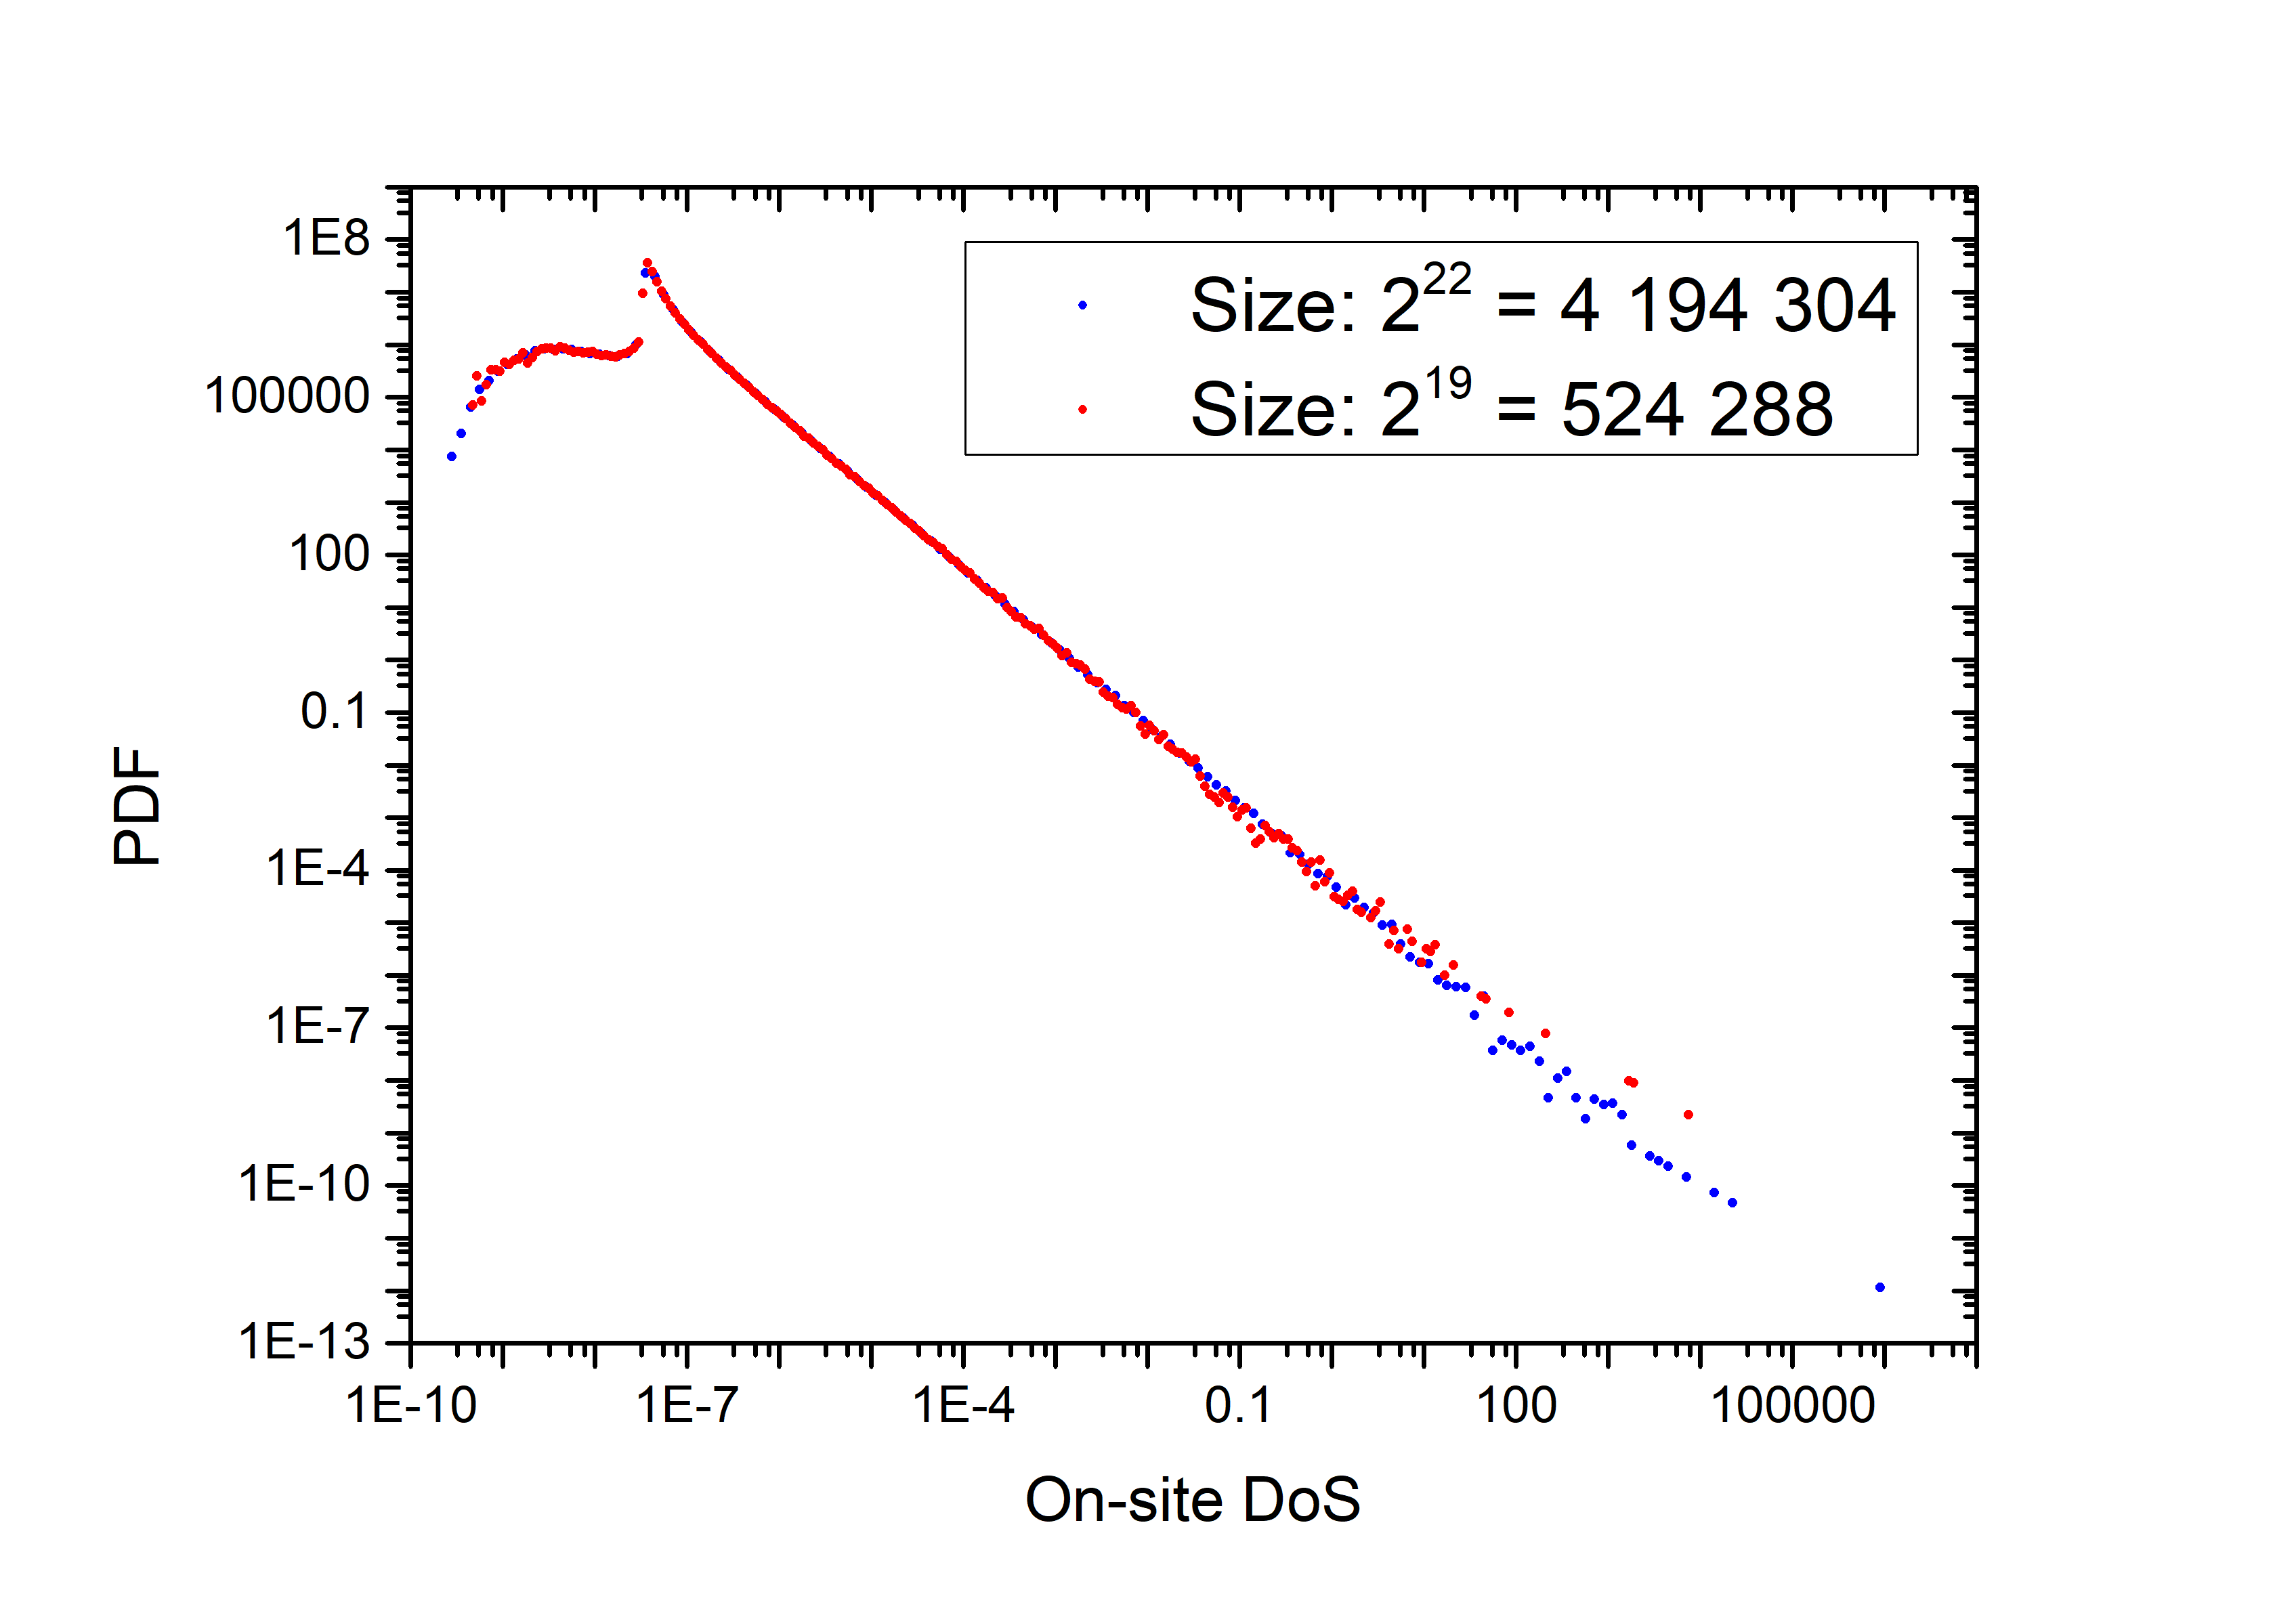
\includegraphics[width=0.8\textwidth]{DOS_disribution_for_various_M.png}
	\caption{Форма стационарного распределения при двух различных значениях параметра $M$ (указаны на рисунке). Значение параметра регуляризации $\gamma = 10^{-7}$. Значения физических параметров см. в тексте}
\end{figure}

Данные зависимости демонстрируют следующие качественные детали влияние параметров $M, \gamma$ на распределение:
\begin{itemize}
	\item При недостаточно малом $\gamma$ этот параметр создаёт резкую отсечку распределения на некотором значении, линейно зависящем от $\gamma$. Это легко понять, посмотрев непосредственно на формулы популяционной динамики \eqref{eq:Population_dynamics_final_equations} и сделав оценки для конкретных чисел:
	\begin{itemize}
		\item значений, больших по модулю, чем 
		$$\frac{g}{K \gamma \Delta} \sim 3 \cdot 10^{8}$$
		возникнуть не может в принципе (это соответствует строго нулевой действительной части и минимально возможному значению мнимой части знаменателя).
		\item В таком случае на следующей итерации значение модуля не может быть меньше
		$$ \left[ \frac{g}{K \gamma \Delta} K \right]^{-1} = \frac{\gamma \Delta}{g} \sim 2 \cdot 10^{-2} \gamma$$
		что мы и наблюдаем на практике с точностью до порядка.
	\end{itemize}
	Эти рассуждения также показывают, что среди экстремальных значений в выборке будет наблюдаться небольшое чередование по номеру итераций между большими и малыми значениями.
	\item Малый размер выборки, как и следует ожидать, оказывает обедняющее воздействие качество статистики на очень больших и очень малых значения плотности состояний. Как мы видели выше, статистика больших и малых значений в рамках этого алгоритма являются связанными: если размер выборки недостаточен для воспроизведения статистически значимых образцов одной области --- тоже самое произойдёт с другой. 
	\item Заметим, что поведение формы распределения объясняет характер поведения среднего и типичного по отношению к различным $\gamma, M$:
	\begin{itemize}
		\item как подсказывает степенная в широких пределах форма распределения (на ней мы ещё остановимся далее), в величину среднего дают доминирующий вклад экстремальные значения в выборке, а потому плохое воспроизведение очень больших значений плотности -- будь то по недостаточно малого $\gamma$ или небольшого $M$ -- приводит к неправильному значению среднего. Также описанные выше рассуждения о чередовании экстремальных значений очевидным образом объясняют наличие в стационарной динамике пиков длинной в одну итерацию.
		\item типичное значение, в отличие от среднего, нечувствительно к <<выбросам>> экстремальных значений, что объясняет слабую чувствительность типичного к размерам выборки.
		Однако, поскольку недостаточно малая $\gamma$ одинаково сильно обрезает оба масштаба, то простой оценкой вида:
		$$
		\rho_{typ} \sim \exp\left\{ \int \limits_{ x_{small} = \sharp \gamma }^{ x_{large} = \sharp \gamma^{-1} } \frac{dx}{x^n} \ln x \right\} \sim \gamma  \exp \left\{ \sharp x_{small}^{1-n} + \sharp x_{large}^{1-n} \right\}
		$$
		легко объяснять, почему типичное также чувствительно к регуляризации $\gamma$.
	\end{itemize}
\end{itemize}
\chapter{Ключевые результаты и их обсуждение} \label{Result}
В этой главе мы изложим результаты численного исследования задачи собственных мод локального оператора \eqref{eq:Local_operator_definition} с единичным собственным числом. Исследование проводилось с помощью подхода, развитого в \autoref{Numer}. В конце мы дадим интерпретацию полученных результатов в терминах изначально исследуемой нами задачи низкоэнергетических возбуждений. 
Нас будут интересовать следующие вопросы:
\begin{itemize}
	\item локальная плотность состояний $\rho$: форма распределения $P(\rho)$, зависимость среднего $\langle \rho \rangle$ и типичного $\exp \langle \ln \rho \rangle$ от параметра $K$ задачи.
	\item свойства локализации состояний: зависимость среднего IPR от параметра $K$ задачи.
\end{itemize}
Необходимые сведения о параметрах симуляций:
\begin{itemize}
	\item постоянные параметры $g = 0.15, \Delta = 2 \exp \left\{ -\frac{1}{g} \right\} \approx 2.55 \cdot 10^{-3}$
	\item Численные значения положения характерных точек, согласно формулам \eqref{eq:K1_definition}-\eqref{eq:K2_definition}:
	\begin{itemize}
		\item точка появления состояний: $K_1 \approx 2$,
		\item точка делокализации состояний: $K_2 \approx 30$
	\end{itemize}
	\item Диапазон доступных для изучения значений параметра $K$ составил $K \in [2, 200]$. При этом достоверные результаты (в обсуждённом ранее в \autoref{Numer} смысле) получены для $K \in [6, 130]$. 
\end{itemize}



\section{Свойства локализации состояний}
Результаты численного исследования показали, что при \textit{всех доступных значениях параметра $K$ состояния являются делокализованными}. Более подробно, результаты таковы:
\begin{itemize}
	\item проверялись значения $K \in [2, 200]$.
	\item факт делокализации устанавливался по зависимости IPR \eqref{eq:IPR_through_GF} от регуляризующего параметра $\gamma$. Пример такой зависимости представлен на Рис. \ref{fig:IPR_and_DOS_dependence_from_gamma} При этом, согласно описанным в \autoref{Numer} подробностям, необходимо следить за стационарностью зависимости локальной плотности состояний, так что пример последней также представлена на Рис. \ref{fig:IPR_and_DOS_dependence_from_gamma}.
	\item Полученные данные наподобие упомянутых позволяют утверждать, что в диапазоне $K \in [4, 130]$ состояния являются делокализованными. Более конкретно, численные свидетельствуют о том, что $IPR(\gamma) \propto \gamma$ во всём диапазоне параметров. В связи с этим, подобные Рис. \ref{fig:IPR_and_DOS_dependence_from_gamma} зависимости для IPR не приводятся --- они все выглядят идентично.
	\item Побочным наблюдением, подтверждающим локализацию, является факт насыщения зависимости типичного значения плотности состояний от $\gamma$, также свидетельствующий о делокализации \cite{AAT}.
	\item Данные явным образом противоречат предсказаниям статьи \cite{FI_microwave}. Причины этих расхождений мы разберём далее.
\end{itemize}

\begin{figure}[h!]
	\label{fig:IPR_and_DOS_dependence_from_gamma}
	\centering
	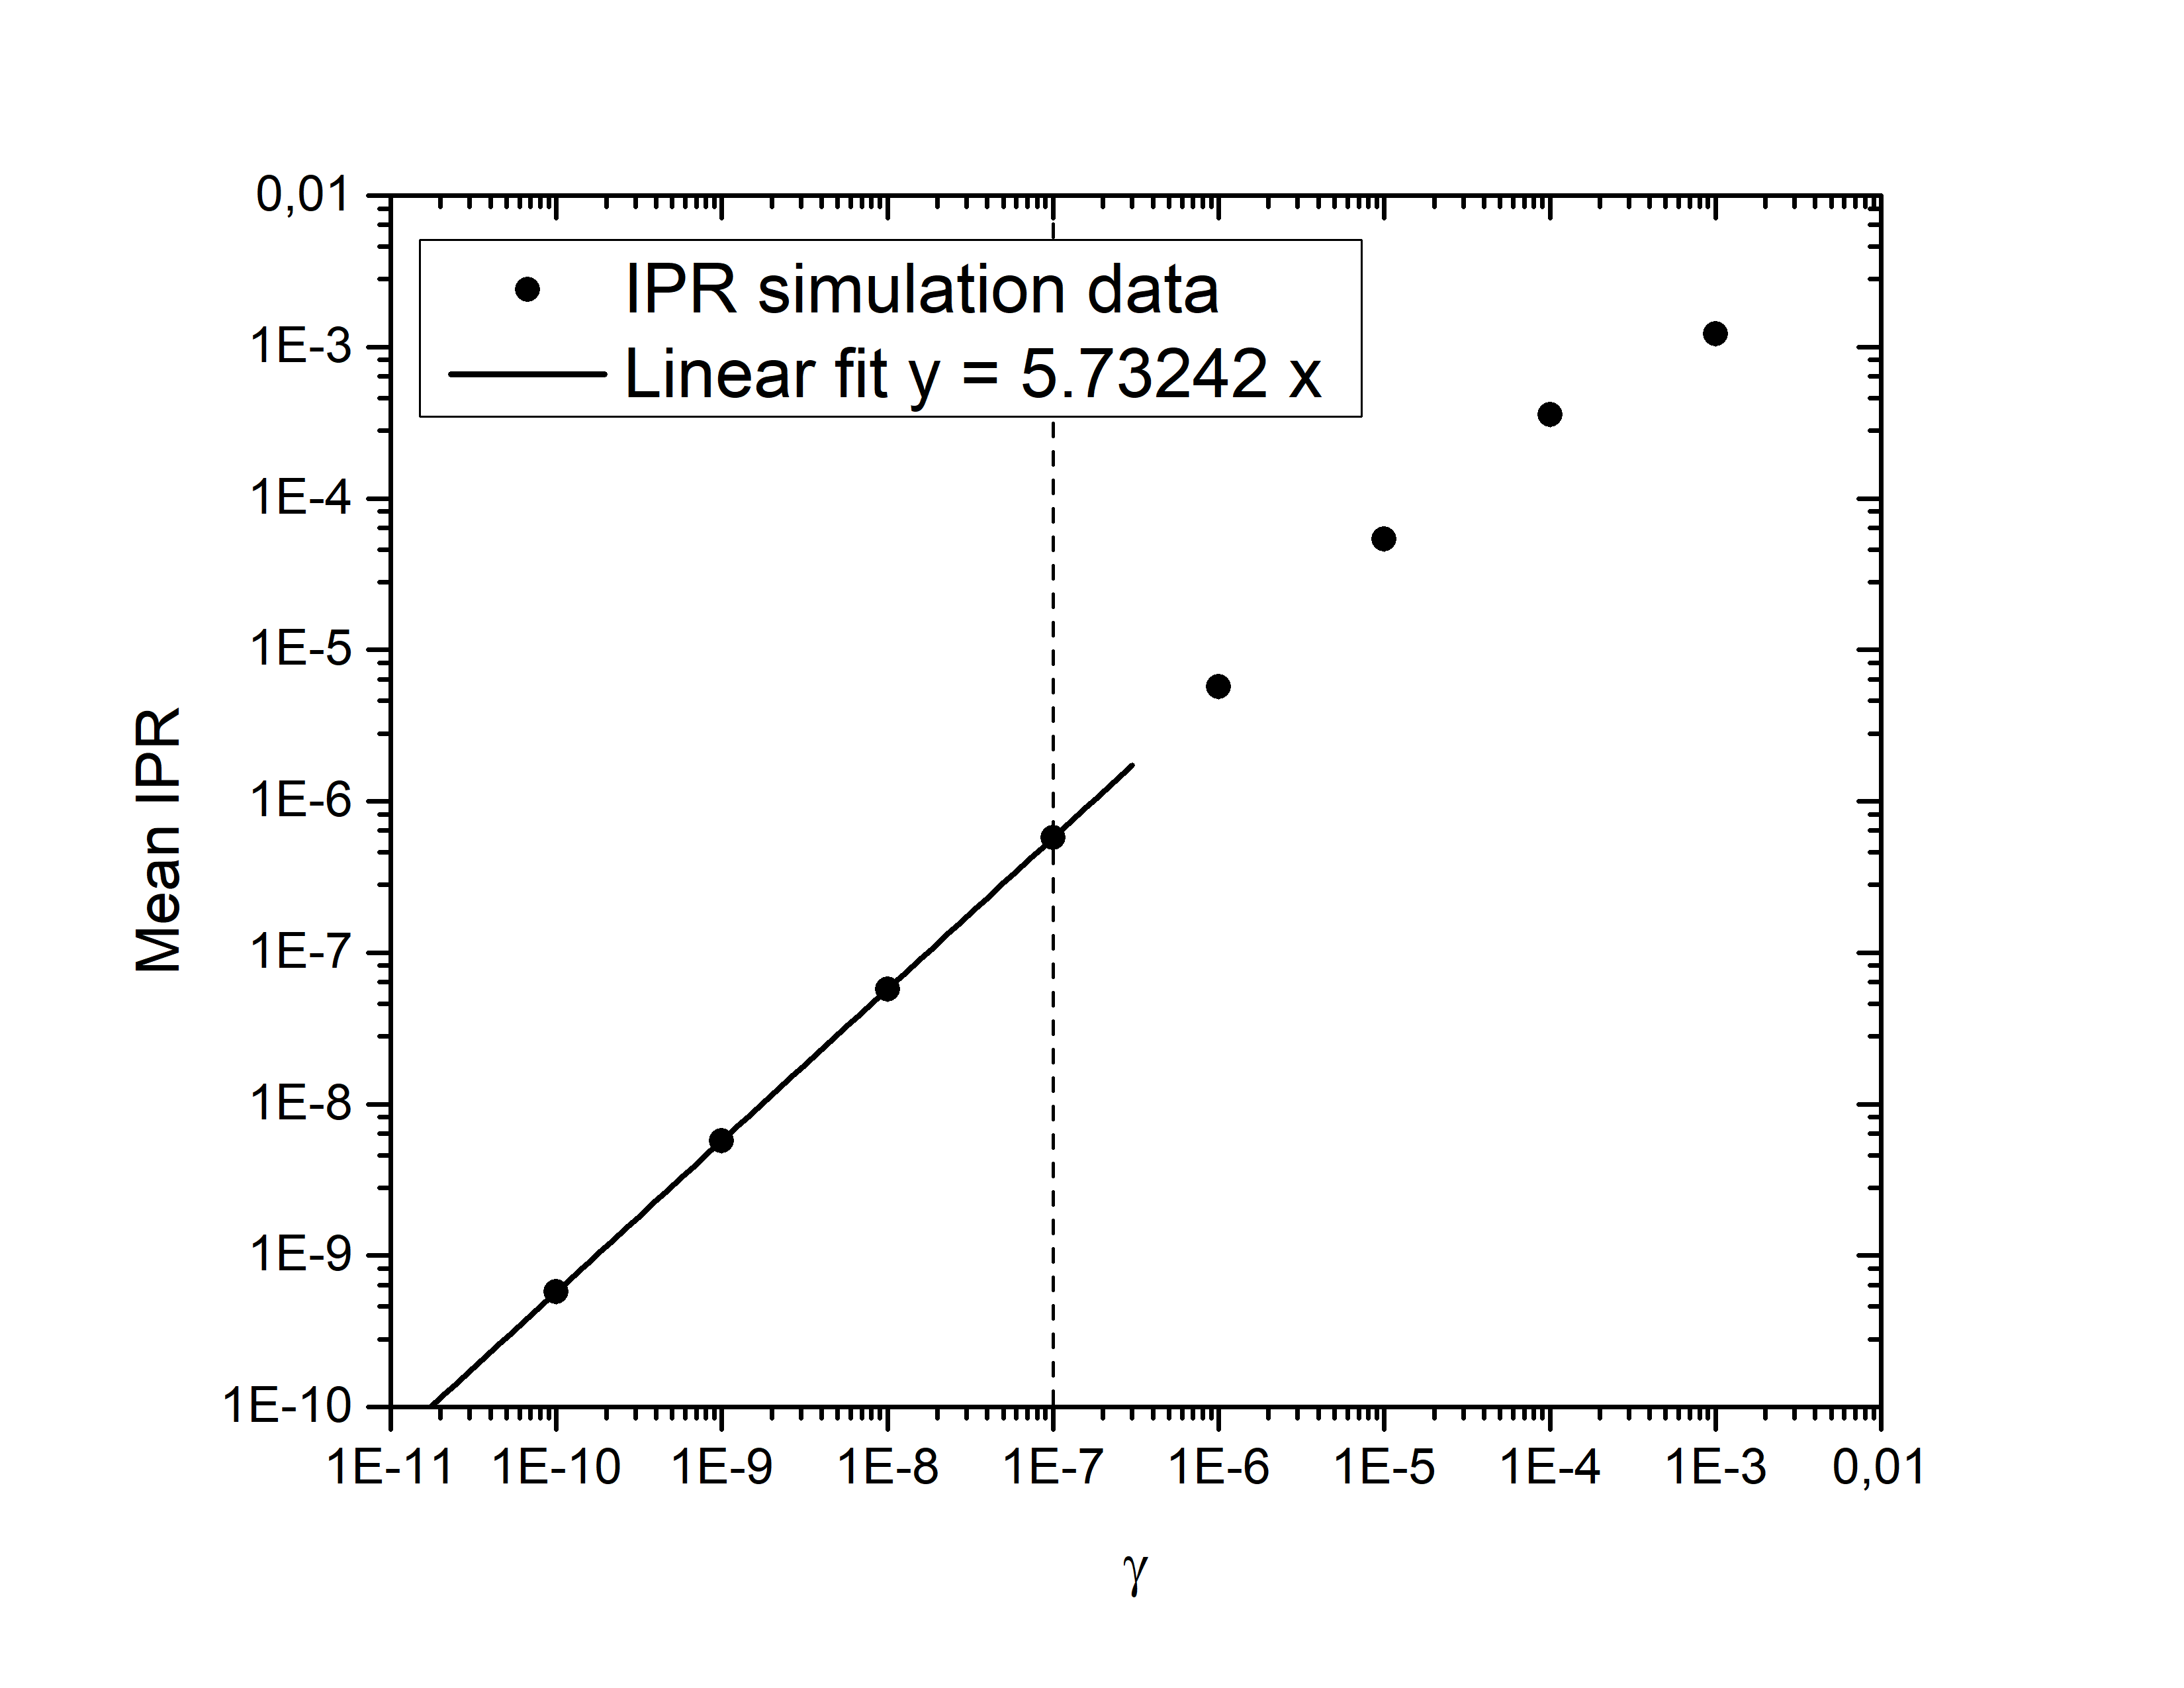
\includegraphics[width=0.49\textwidth]{Mean_IPR_gamma_dependence.png}
	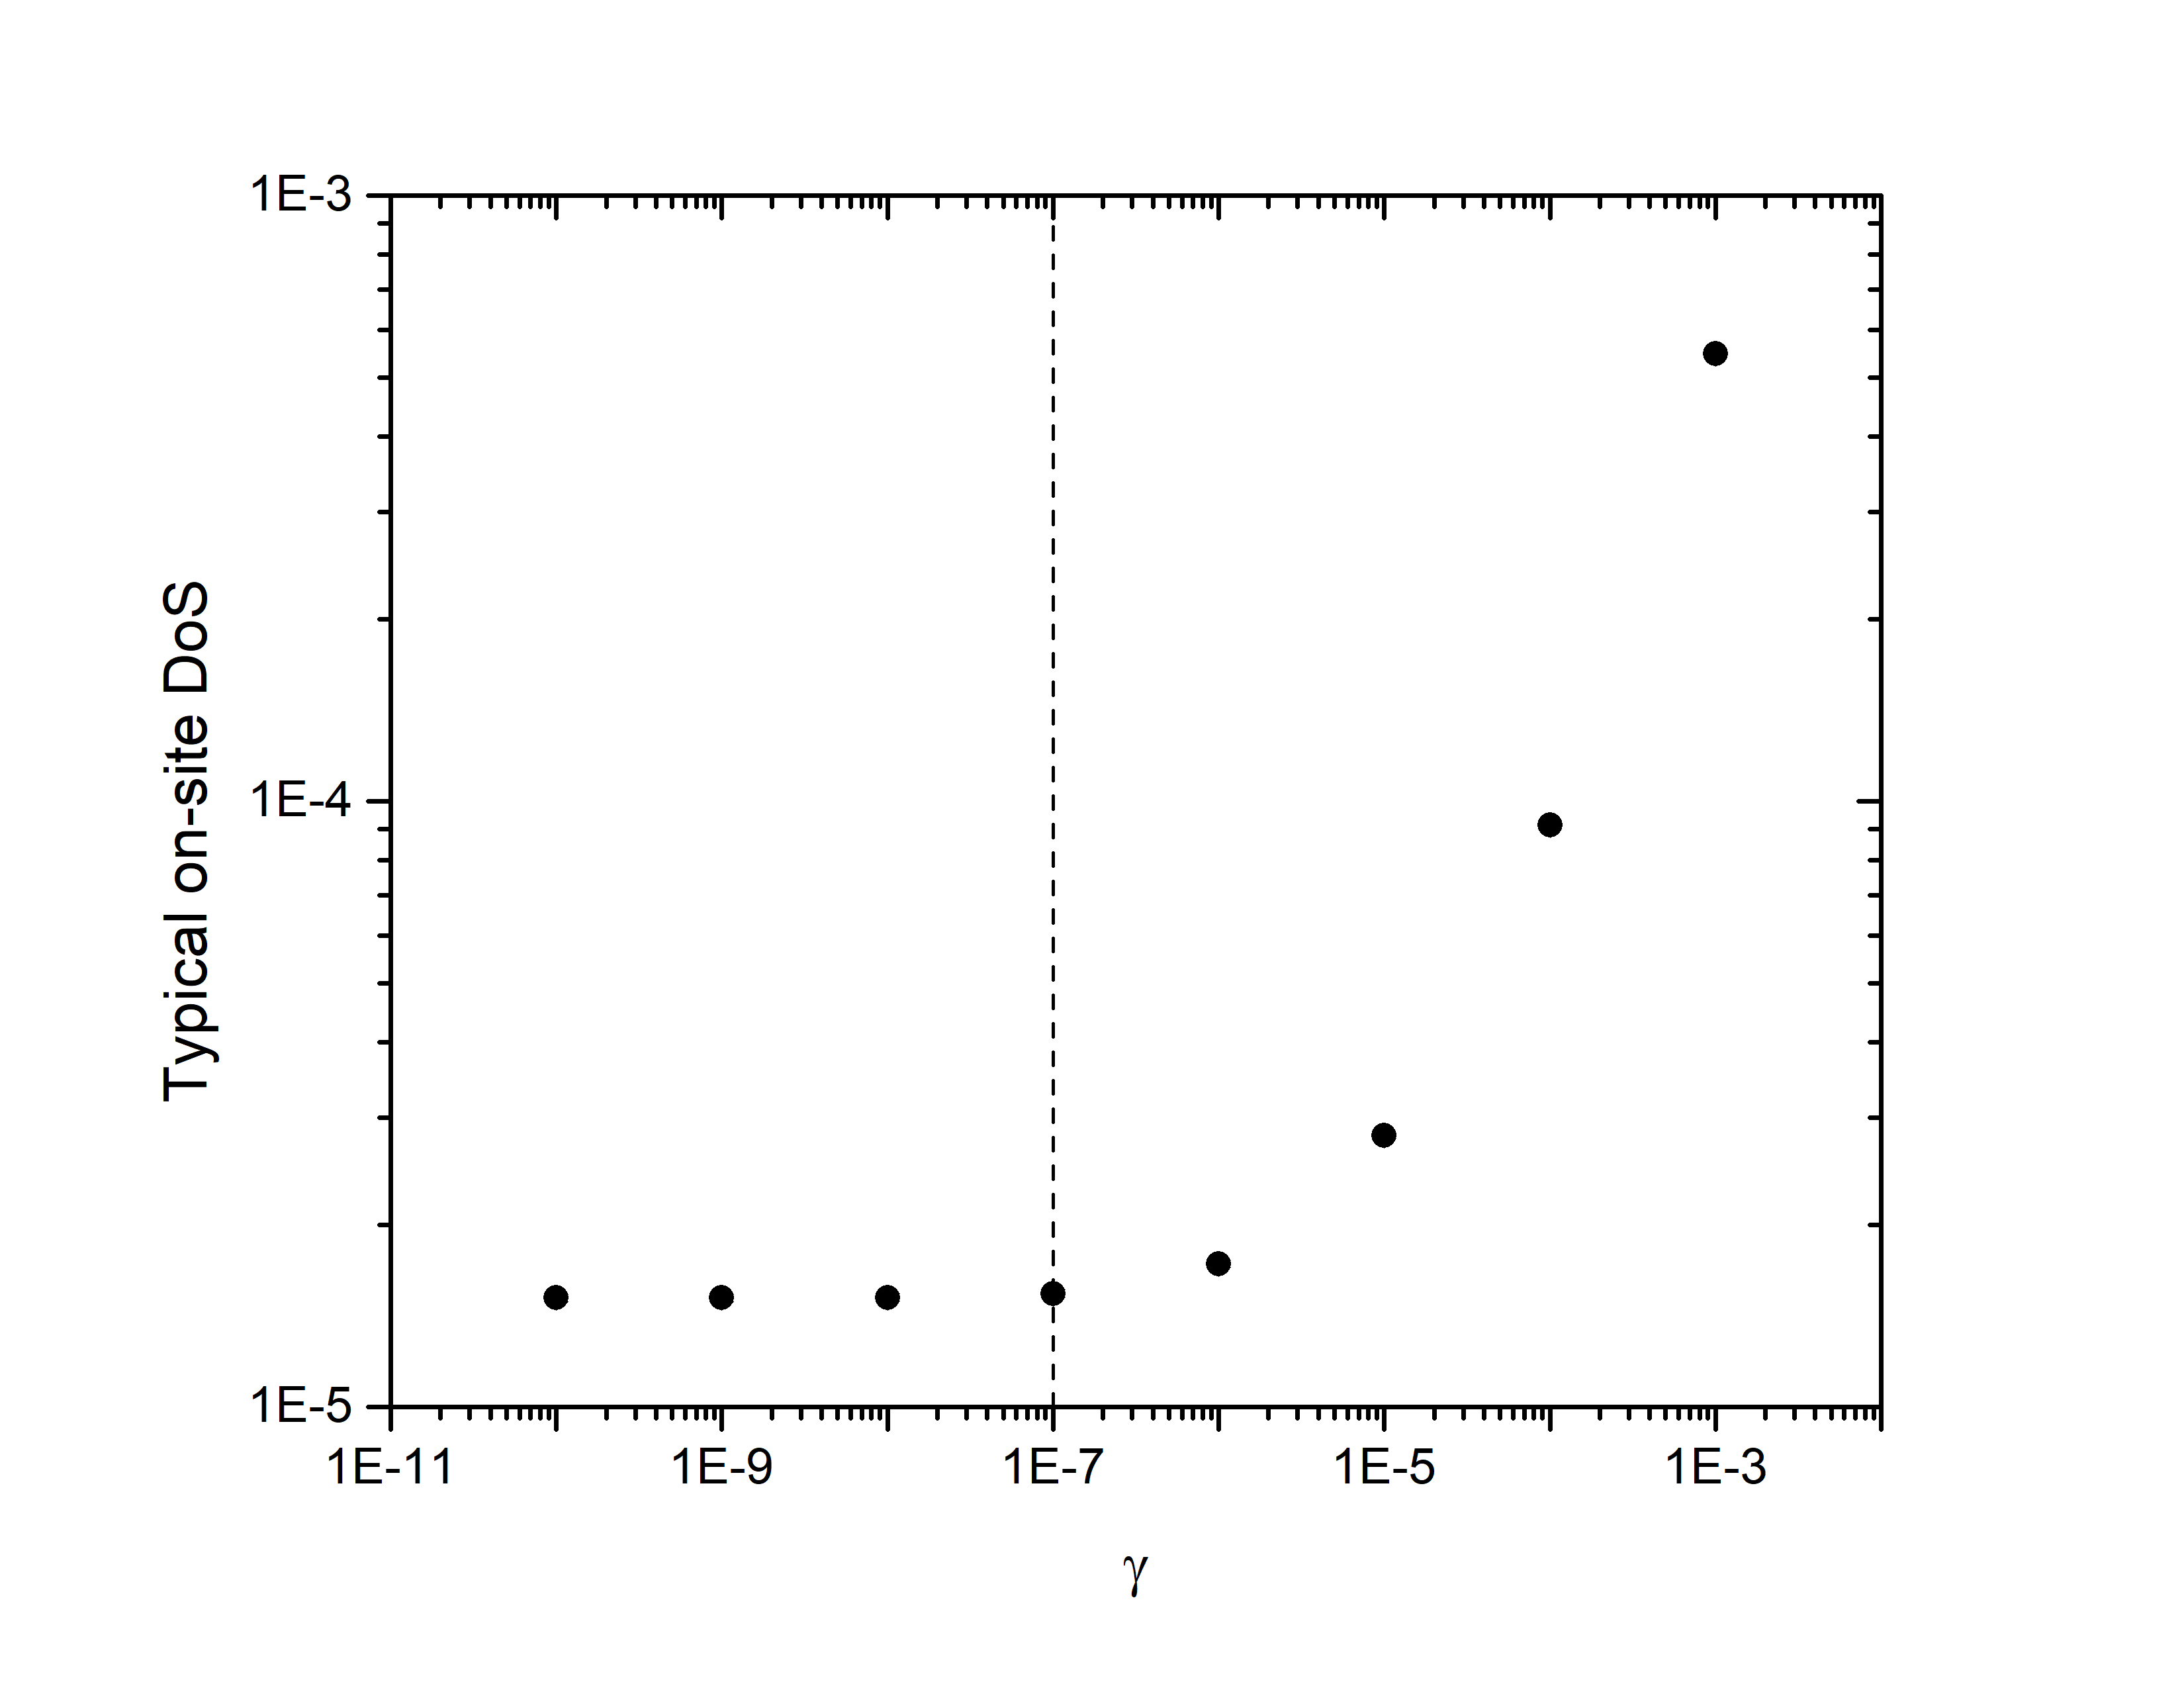
\includegraphics[width=0.49\textwidth]{Typical_DOS_gamma_dependence_for_IPR.png}
	\caption{Зависимость средней IPR (слева) и типичной плотности состояний (справа) от регуляризующего параметра $\gamma$. На обоих зависимостях пунктирной линией отмечено значение $\gamma$ насыщения типичной плотности состояний. Зависимость средней IPR от $\gamma$ сопровождается также графиков линейной аппроксимации в зоне насыщения. Параметры симуляции: $K = 30, M = 2^{25} \approx 3.4 \cdot 10^{8}$.}
\end{figure}



\section{Распределение мнимой части модельной функции Грина}
Рассмотрим далее уже не раз упоминавшуюся форму распределения плотности состояний. К обсуждению предлагается пример на Рис. \ref{fig:DOS_distribution_example} со следующими параметрами:
\begin{itemize}
	\item физические параметры $K = 15, g = 0.15, \Delta = 2 \exp\left\{ -\frac{1}{g} \right\}$;
	\item параметры алгоритма $M = 2^{25} \approx 3.4 \cdot 10^{8}, \gamma = 10^{-10}$.
\end{itemize}
Отметим, что в целом больших различий в качественных характеристиках этой формы при различных $K$ замечено не было, поэтому все важные особенности могут быть продемонстрированы на приведённом Рис. \ref{fig:DOS_distribution_example}. Также это означает, что показательным являются зависимости численных характеристик этого распределения, которые будут активно обсуждаться далее. 

\begin{figure}[h!]
	\label{fig:DOS_distribution_example}
	\centering
	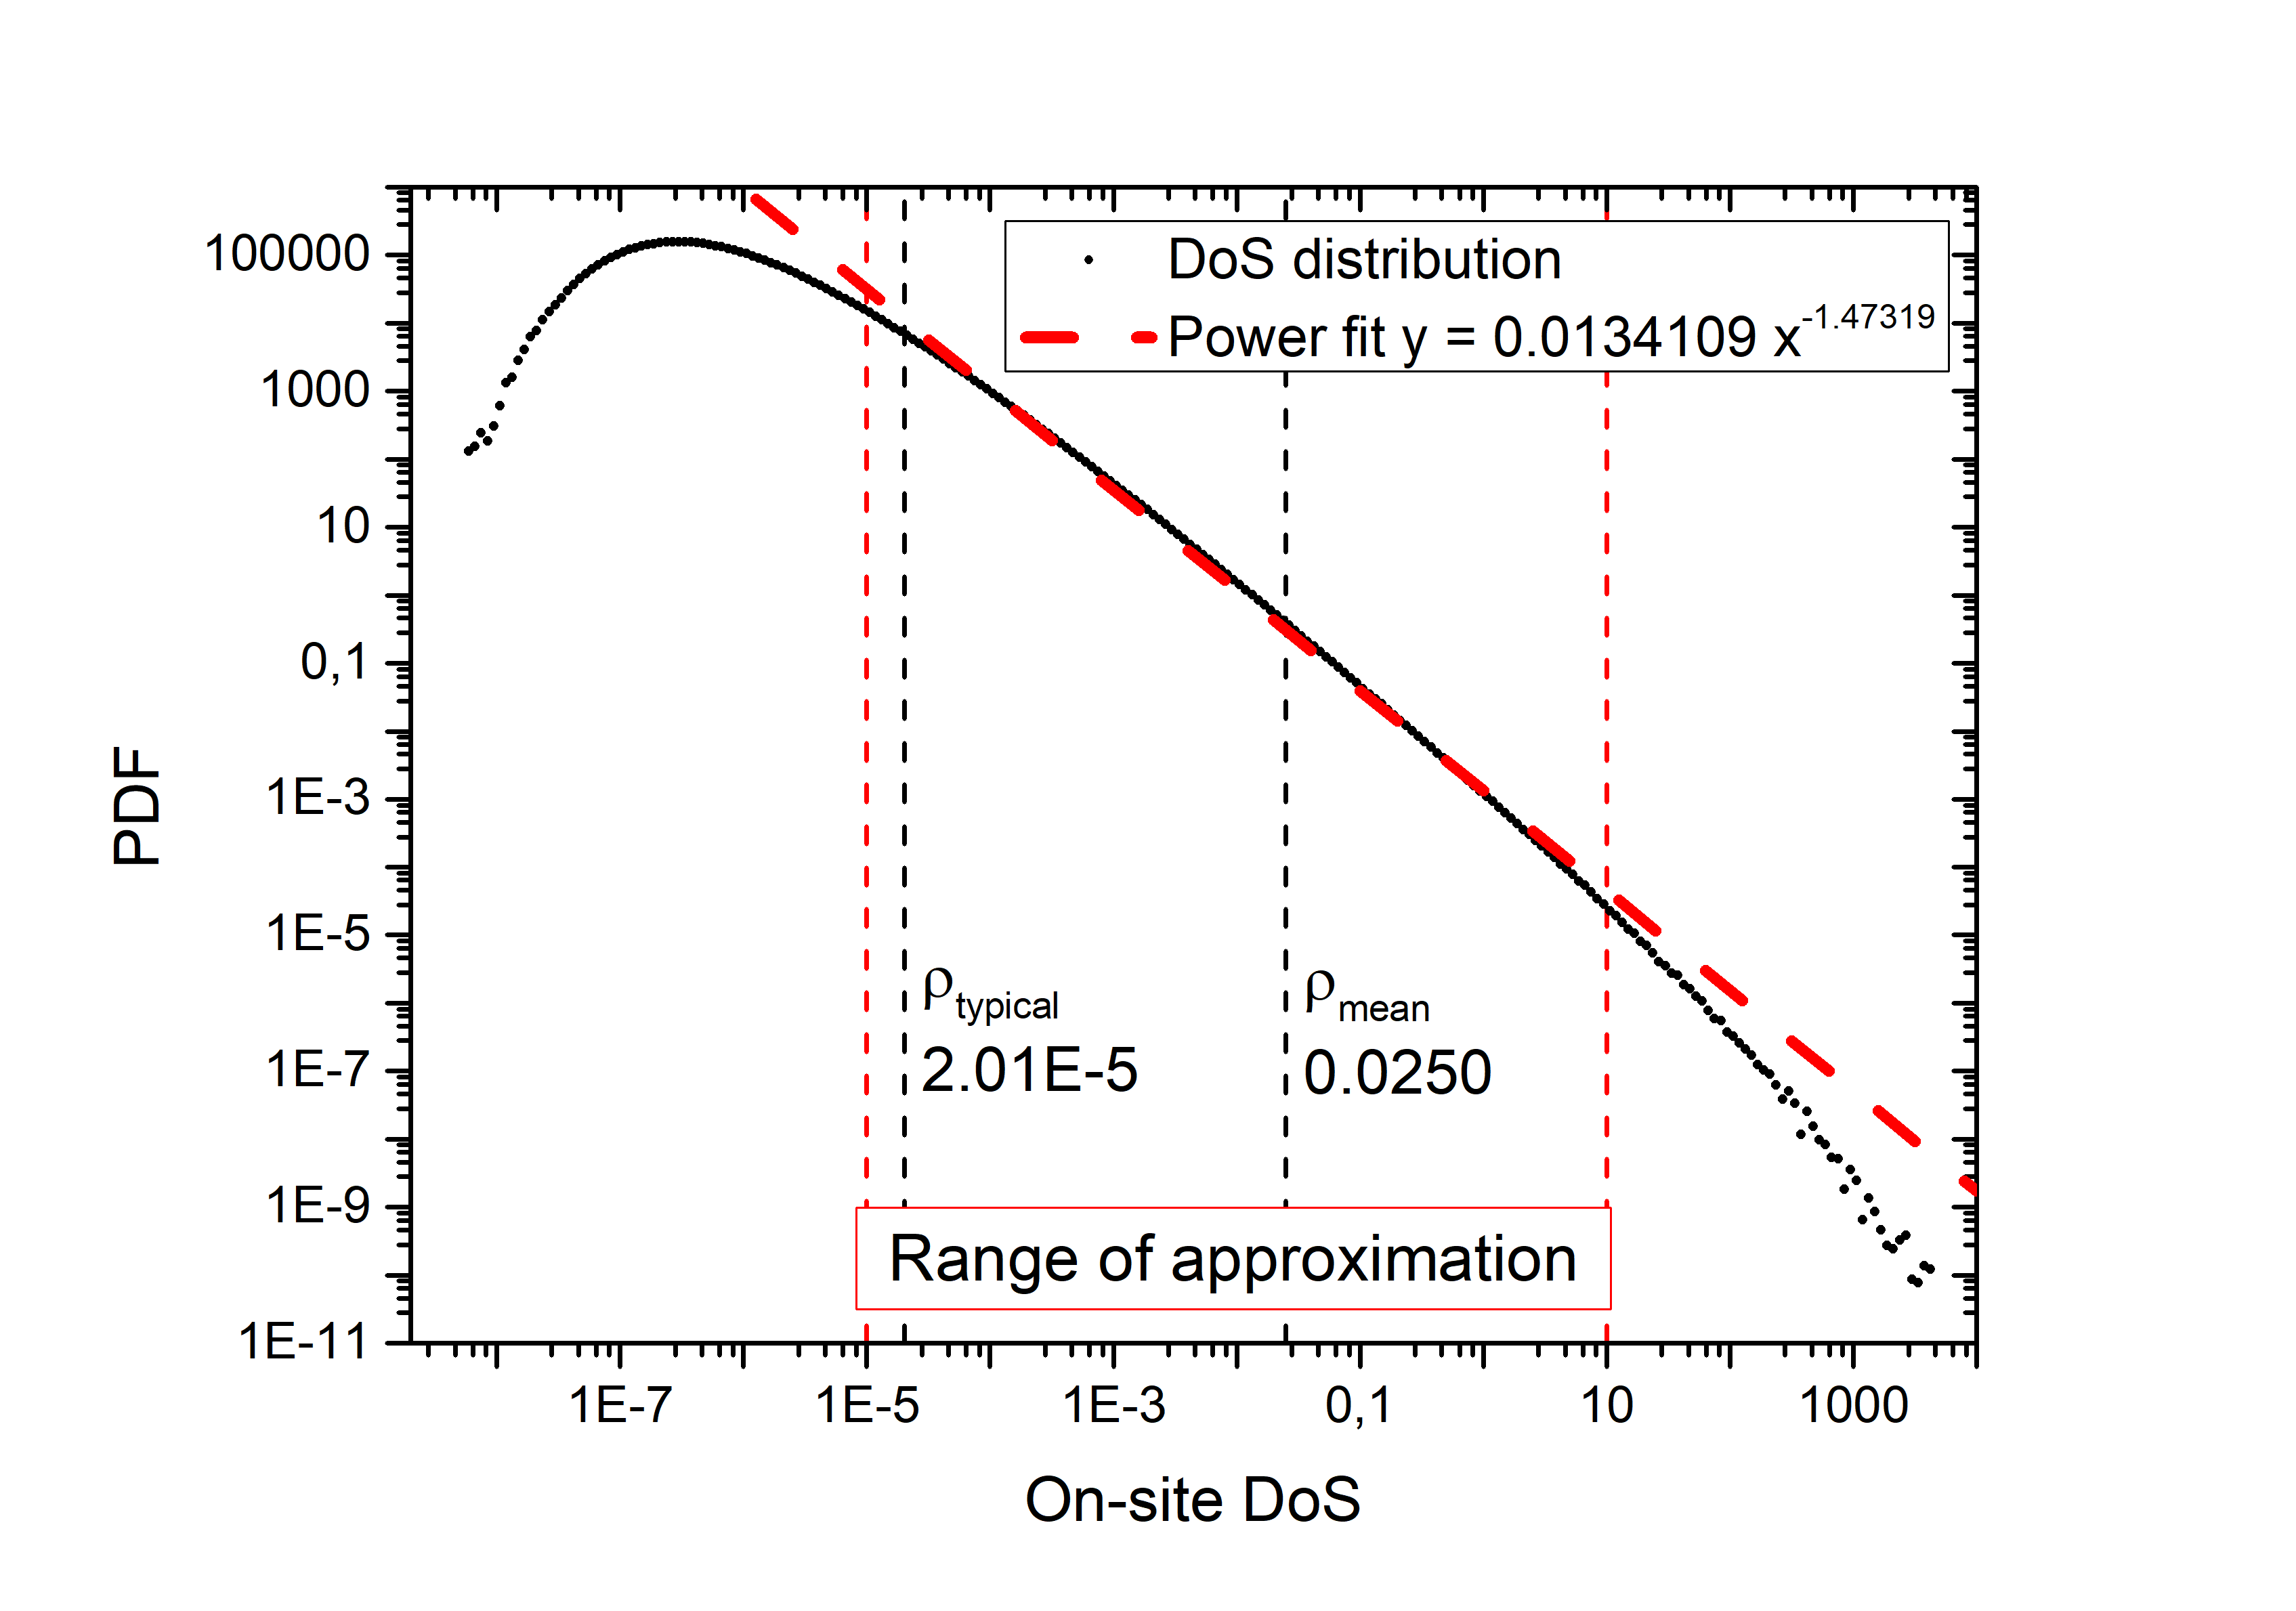
\includegraphics[width=0.9\textwidth]{DOS_distribution_example.png}
	\caption{Распределение локальной плотности состояний. Параметры см. в тексте. На графике также изображена степенная аппроксимация секции распределения, ограниченная красными пунктирными линиями. Вид зависимости для аппроксимации также указан на графике. Чёрными пунктирными линиями показаны характеристики распределения -- средняя и типичная плотность состояний с соответствующими численными значениями.}
\end{figure}

Зафиксируем наблюдаемые особенности распределения и следствия из них. Ещё раз подчеркнём, что эти особенности наблюдаются \textit{во всём диапазоне значений параметра $K$}:
\begin{enumerate}
	\item прежде всего, заметим, что в широких пределах поведение распределения является степенным, причём аппроксимация показывает значение показателя, близкое к $3/2$, т. е. распределение имеет <<длинный хвост>>.
	\begin{itemize}
		\item Важно заметить ещё одно обстоятельство, связанное с уже упомянутым соотношением рассматриваемой задачи с задачей Андерсона с диагональным беспорядком: наблюдаемый показатель степени очень близок к критическому показателю, наблюдаемым ровно на пороге локализации \cite{AAT}. Как мы продемонстрируем несколько позже, данное совпадение не случайно.
	\end{itemize}
	\item Степенное поведение реализуется в очень широких пределах: диапазон составляет минимум 6 порядков.
	\item Среднее $\langle \rho \rangle \approx 2.5 \cdot 10^{-2}$ и типичное $\exp \langle \ln \rho \rangle  \approx 2.5 \cdot 10^{-2}$  для данного распределения отличаются на три порядка. Данное поведение легко понять на основе уже упомянутого степенного поведения распределения:
	\begin{itemize}
		\item само распределение в широких пределах $\rho_{min} \ll \rho \ll \rho_{max}$ имеет степенной вид, из чего можно оценить его нормировку:
		$$
		P(x) \sim A x^{-3/2} \Rightarrow A \sim \left[ \int \limits_{ \rho_{min} }^{ \rho_{max} } \frac{dx}{x^{3/2}} \right]^{-1} \sim \frac{1}{2} \sqrt{\rho_{min}}
		$$
		Эта нормировка выходит чувствительной к нижней отсечке распределения, которая является наиболее часто выпадающей. По порядку полученная оценка хорошо описывает наблюдаемое поведение: $\frac{1}{2} \sqrt{ \rho_{min} } \sim 2 \cdot 10^{-3}$, что неплохо соотносится с результатами аппроксимации.
		\item В таком распределении среднее значение оценивается как
		$$
		\langle \rho \rangle \sim \int \limits_{ \rho_{min} }^{ \rho_{max} } \frac{A dx}{x^{1/2}} \sim 2 A \sqrt{\rho_{max}} \sim \sqrt{\rho_{max} \rho_{min}} 
		$$
		Результат показывает, что среднее набирается на экстремальных значениях распределения: частота выпадения больших значений довольно мала, и тем не менее, их обрезка явно входит в ответ. Данная формула находит отражение на \ref{fig:DOS_distribution_example}: в логарифмическом масштабе среднее находится примерно посредине между границами степенной зависимости, в соответствии с полученной оценкой. 
		\begin{itemize}
			\item Полученная оценка объясняет уже отмеченные ранее в \autoref{Numer} детали поведения этой величины в рамках численного счёта: при плохом выборе $\gamma, M$ обрезки диктуются не свойствами системы, а этими параметрами внутренними параметрами. При этом нижняя граница фиксированна величиной $\gamma$, а верхняя сильно флуктуирует из-за малого размера выборки, что приводит к появлению в динамике алгоритма уже описанных <<выбросов>>.
		\end{itemize}
		\item Для типичного подобные рассуждения приводят к уже анонсированному ранее результату
		$$
		\rho_{typ} \sim \exp\left\{ \int \limits_{ \rho_{min} }^{ \rho_{max} } \frac{A dx}{x^{3/2}} \ln x \right\} \sim \exp\left\{ 2 A \left( 2 + \ln \rho_{min} \right) \frac{1}{ \sqrt{\rho_{min}} } \right\} \sim \rho_{min}
		$$
		Такие оценки демонстрируют, что в отличие от среднего, типичное, как и нормировка распределения, набирается на малых значениях $\rho$, что можно усмотреть и на Рис. \ref{fig:DOS_distribution_example}: типичное по значению близко к границе степенного поведения.
		\item Можно оценить различие среднего и типичного:
		$$ \frac{ \langle \rho \rangle }{ \rho_{typ} } \sim \sqrt{\frac{ \rho_{max} }{ \rho_{min} }} $$
		Для видимого отношения обрезок $\sim 10^6$ получаем наблюдаемое отношение среднего и типичного $\sim 10^3$.
	\end{itemize}
\end{enumerate}



\section{Зависимость физических величин от параметра $K$}
Наконец, мы подошли к главному количественному результату нашей работы: в этом разделе мы приведём зависимости средней и типичной плотности состояний от $K$, и на основании этих зависимостей построим фазовую диаграмму для исследуемой модели. Неизменные параметры всё те же: $g = 0.15, \Delta = 2 \exp \left\{ -\frac{1}{g} \right\}$.


\subsection{Зависимости от параметра $K$}

\begin{figure}[h!]
	\label{fig:Mean_DOS_dependence_from_K}
	\centering
	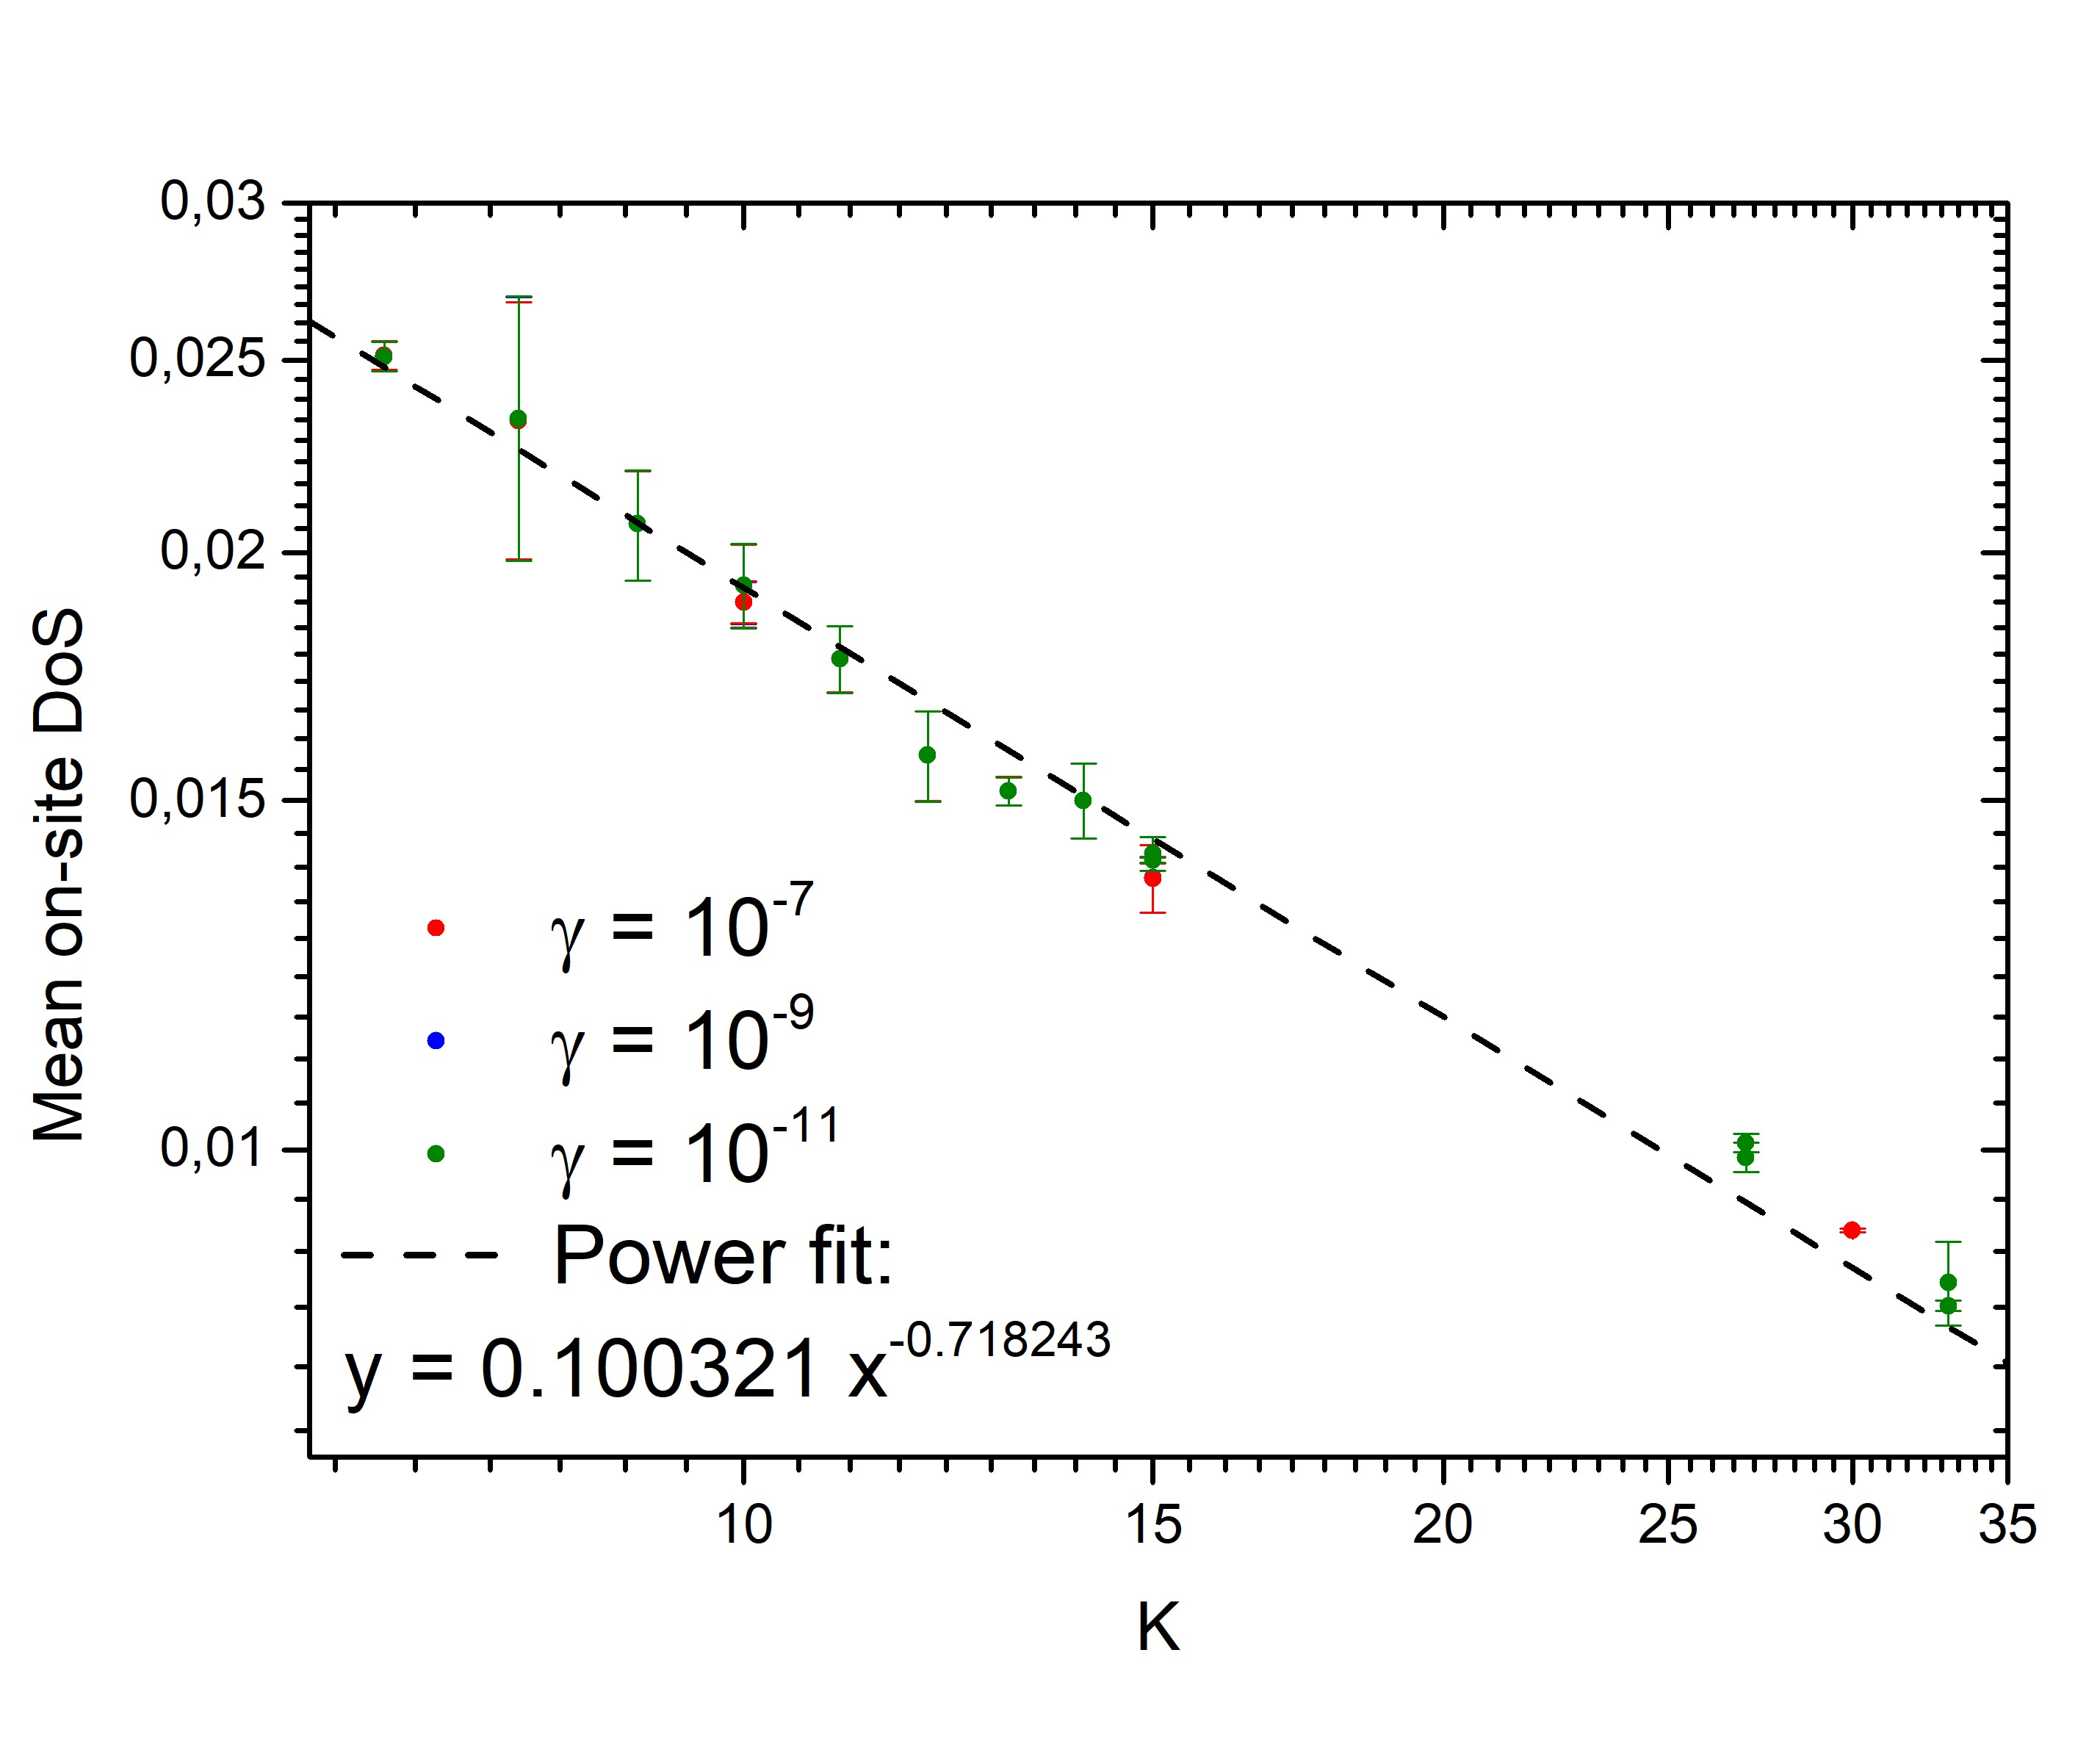
\includegraphics[width=0.49\textwidth]{Mean_DOS_dependence_K_small.jpg}
	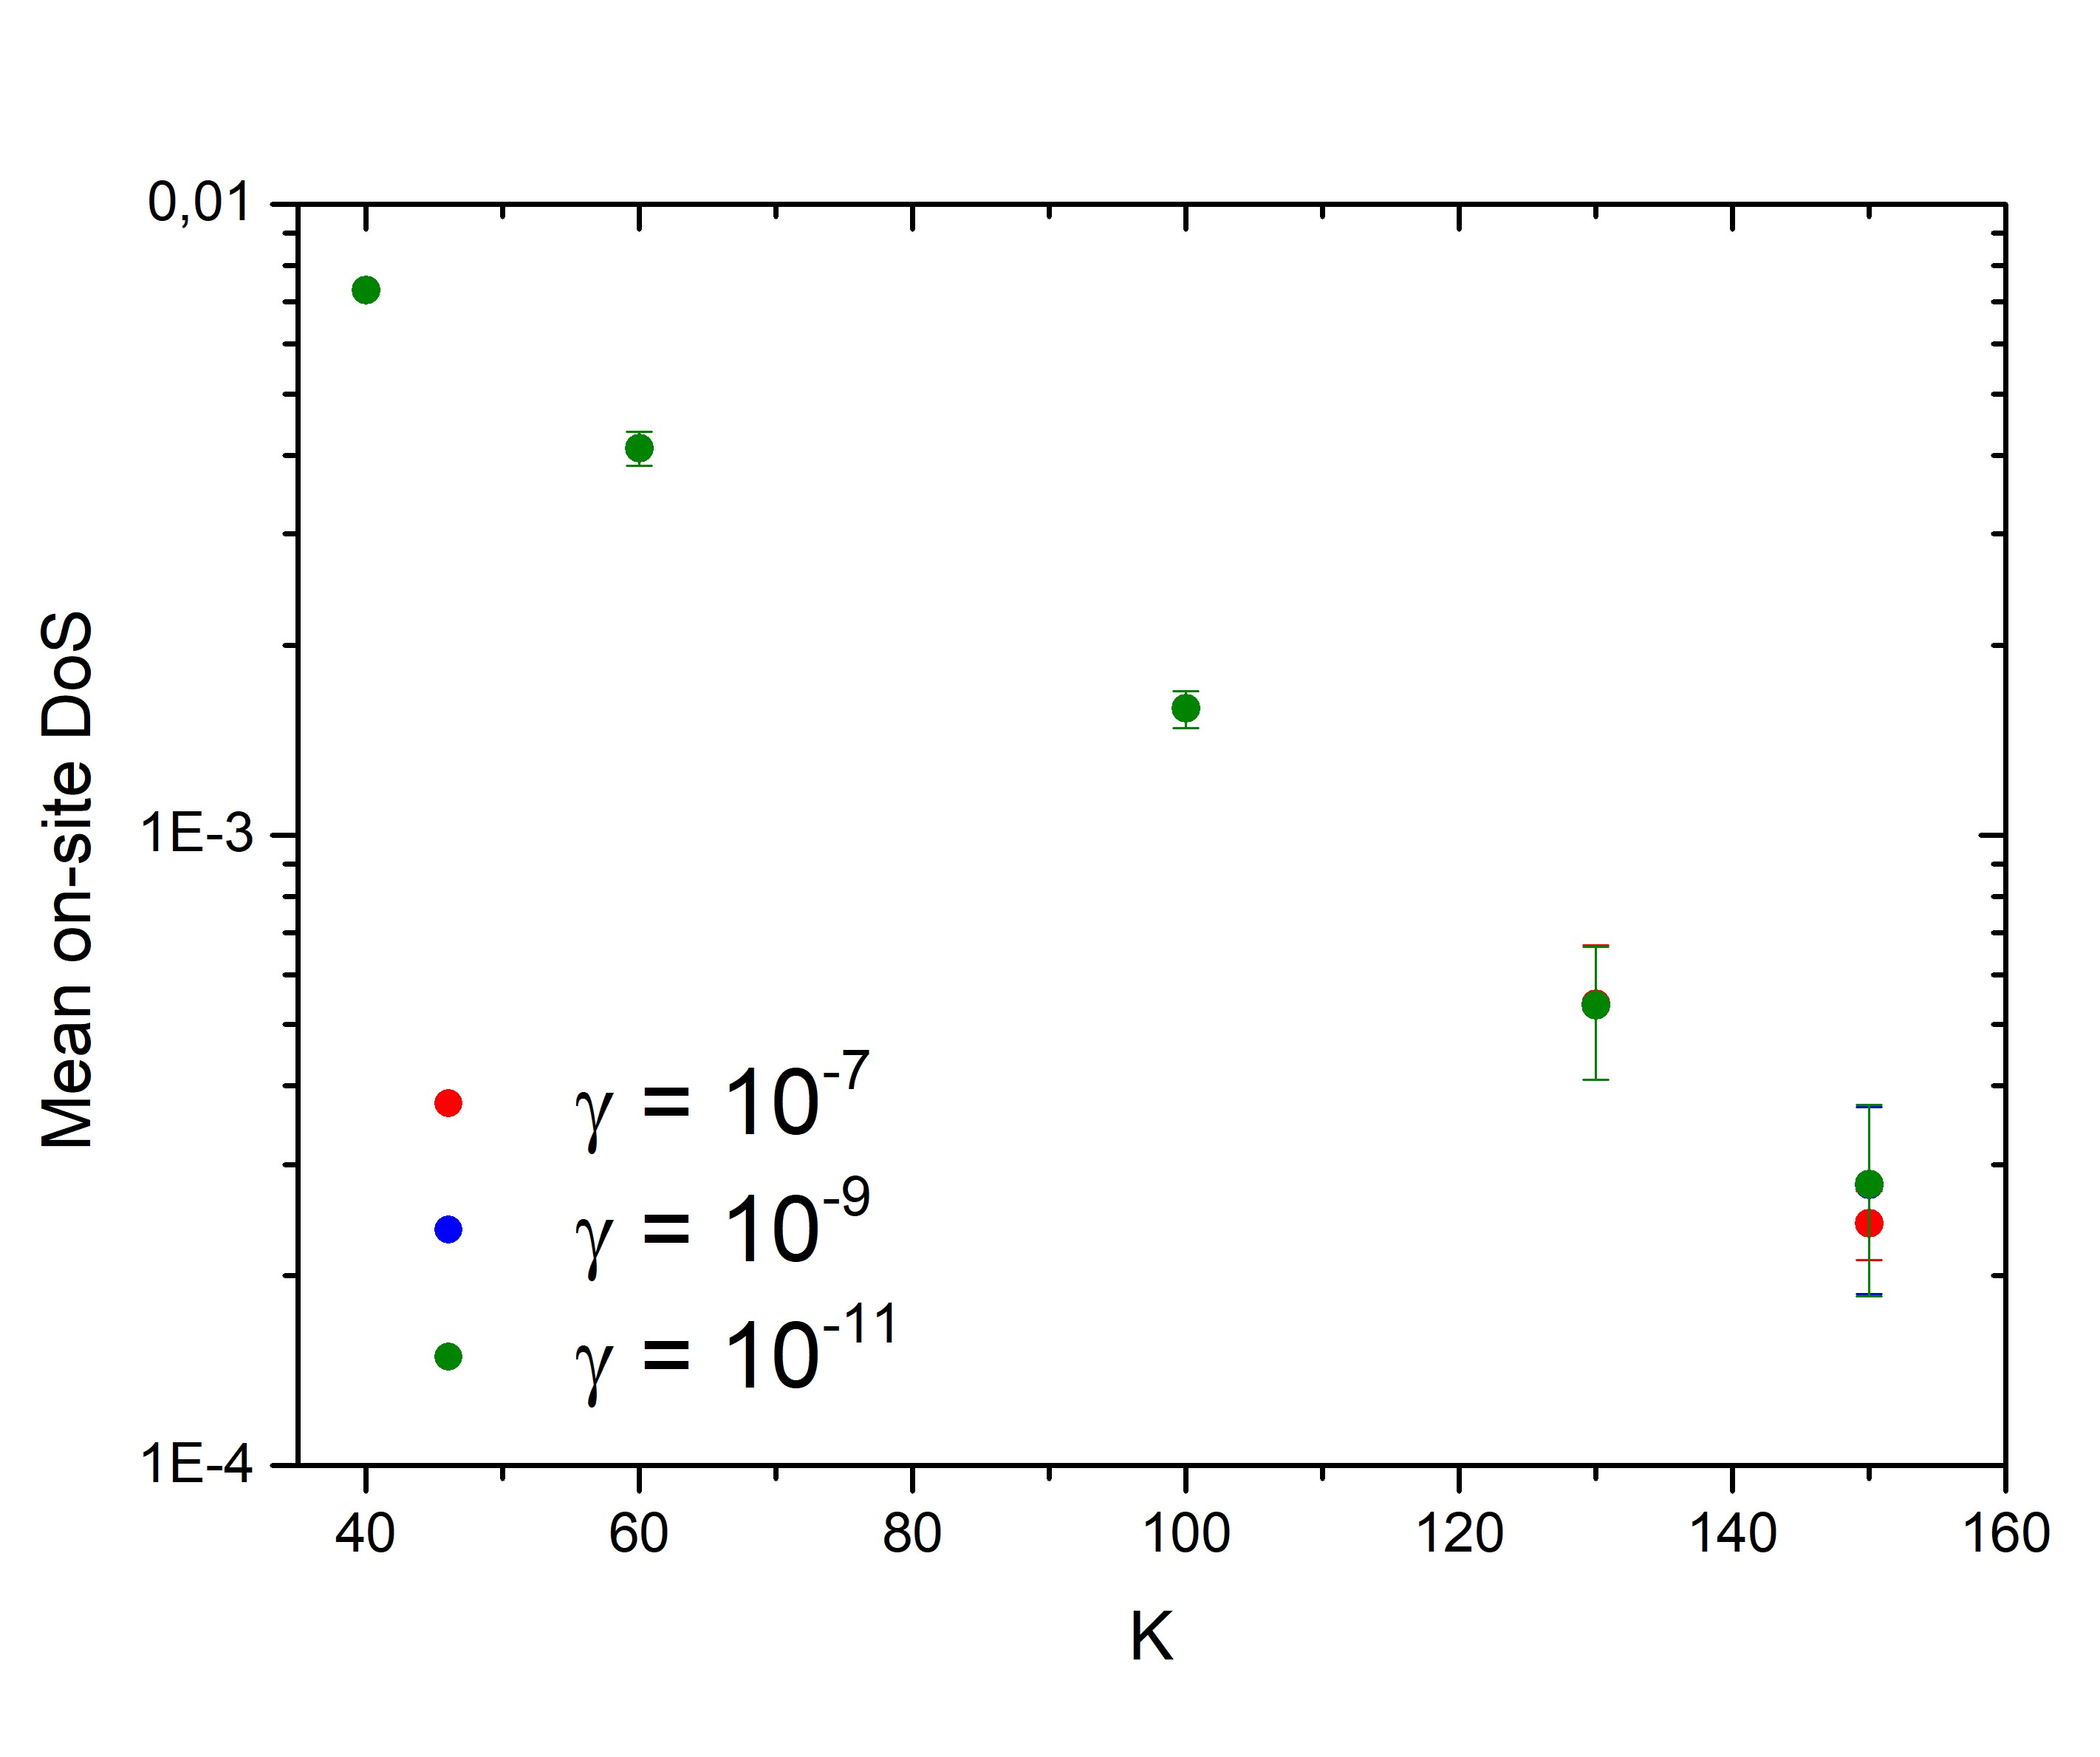
\includegraphics[width=0.49\textwidth]{Mean_DOS_dependence_K_large.jpg}
	\caption{Зависимость средней плотности состояний $\langle \rho \rangle$ от числа ветвления $K$. Данные разделены на две части, отображаемые в разных масштабах: малые $K < 35$ построены в масштабе $LogX, LogY$, а большие $K > 35$ --- $LinX, LogY$. На рисунке представлены версии зависимостей для трёх различных значений параметра $\gamma$. Наличие нескольких точек при данном значении $K, \gamma$ соответствует разным размерам выборки $M$. Область малых значений $K < 35$ также оснащена степенной аппроксимацией данных.}
\end{figure}

\begin{figure}[h!]
	\label{fig:Typical_DOS_dependence_from_K}
	\centering
	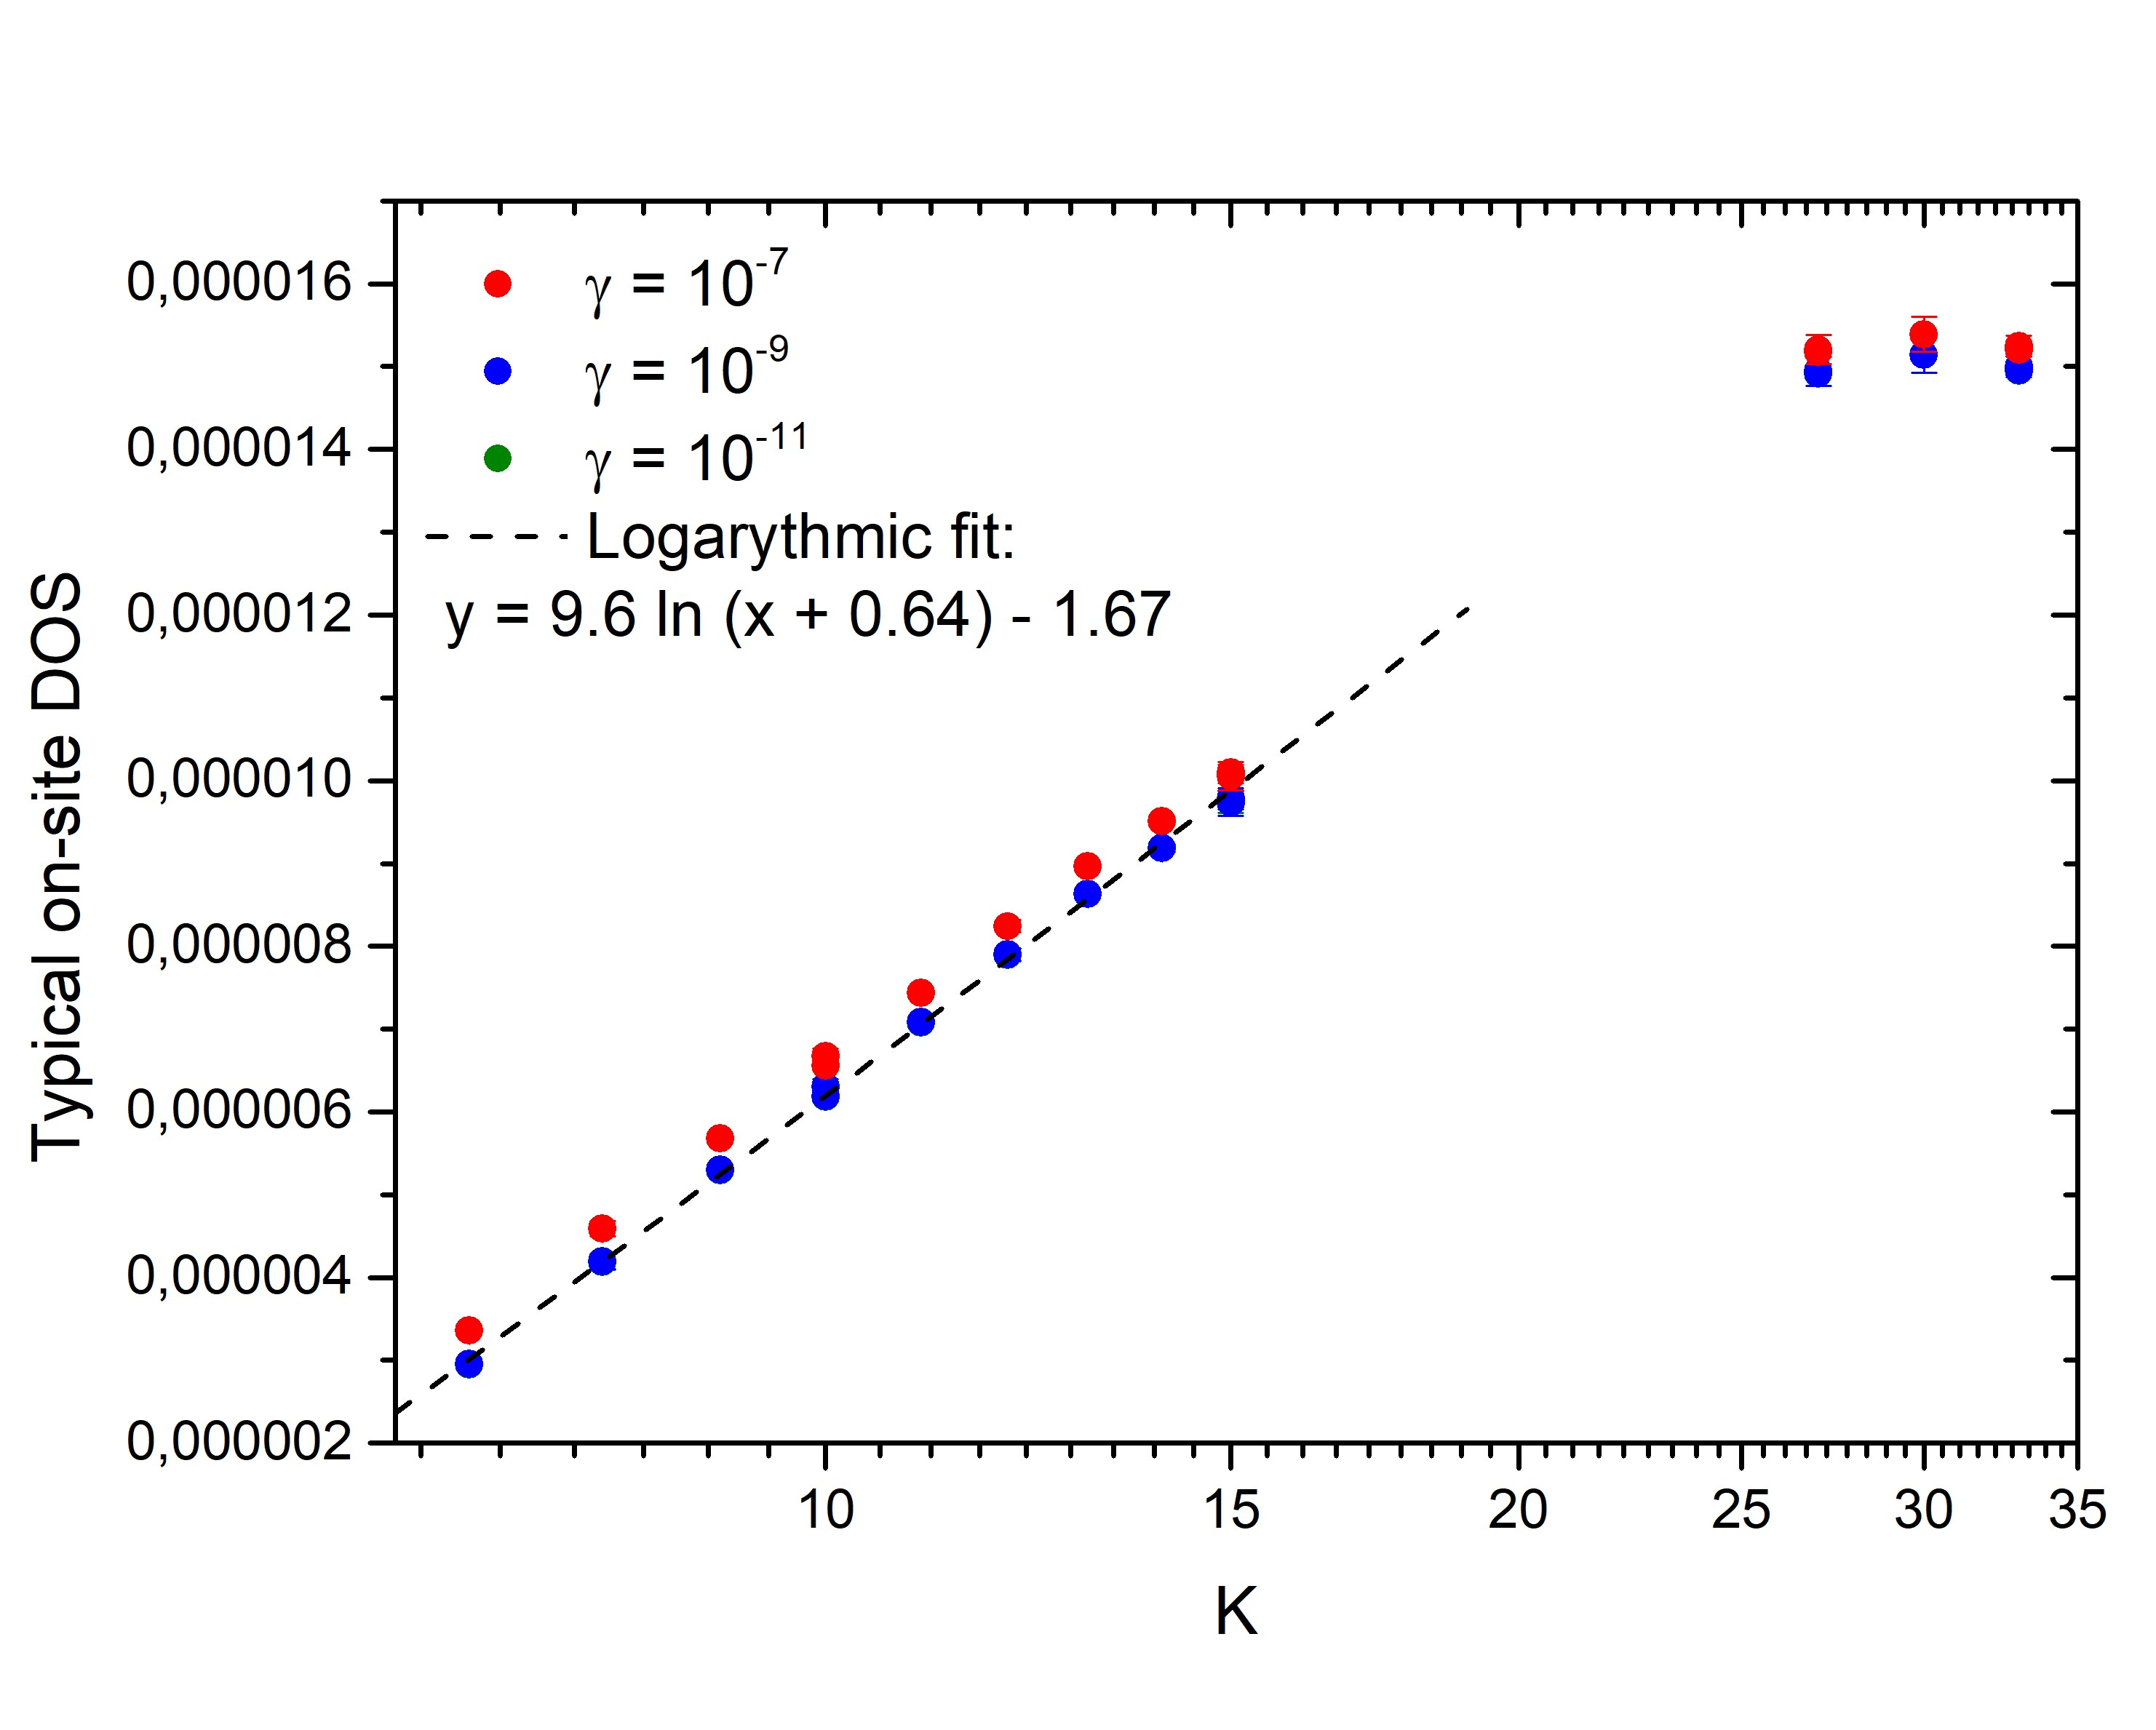
\includegraphics[width=0.49\textwidth]{Typical_DOS_dependence_K_small.jpg}
	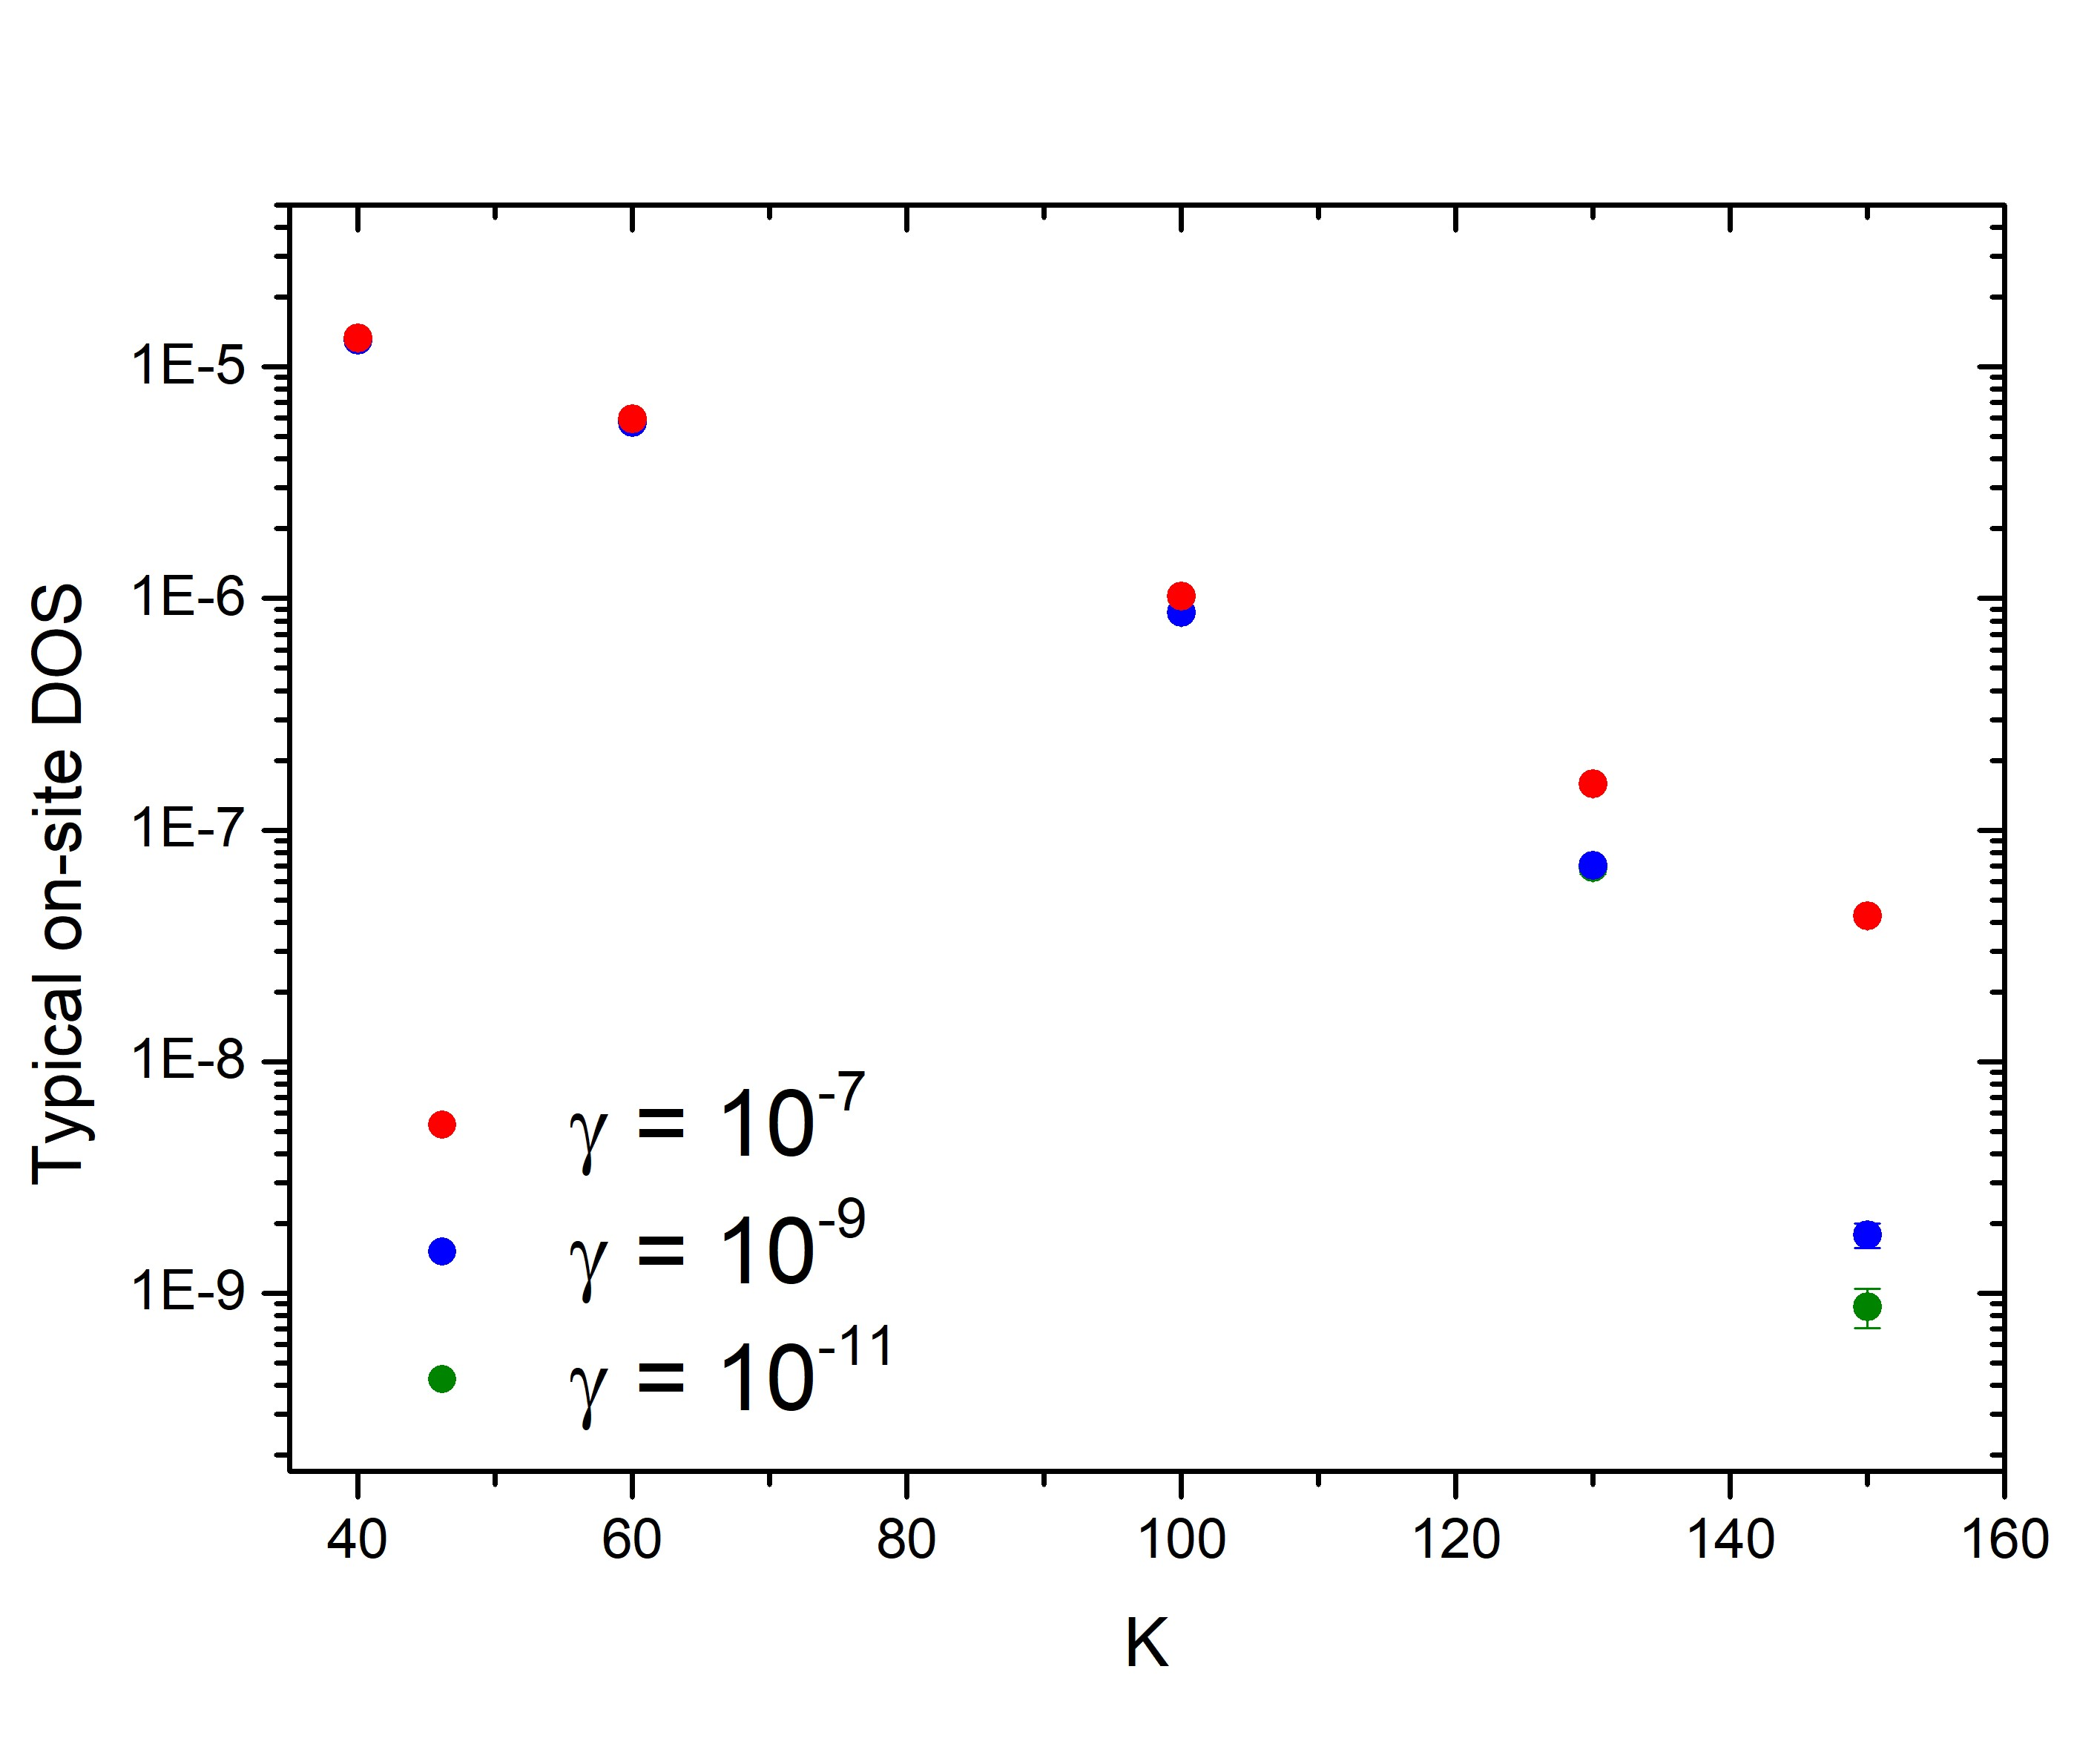
\includegraphics[width=0.49\textwidth]{Typical_DOS_dependence_K_large.jpg}
	\caption{Зависимость типичной плотности состояний $\exp \langle \ln \rho \rangle$ от числа ветвления $K$. Данные разделены на две части, отображаемые в разных масштабах: малые $K < 35$ построены в масштабе $LogX, LinY$, а большие $K > 35$ --- $LinX, LogY$. На рисунке представлены версии зависимостей для трёх различных значений параметра $\gamma$. Наличие нескольких точек при данном значении $K, \gamma$ соответствует разным размерам выборки $M$. Область малых значений $K < 35$ также оснащена логарифмической аппроксимацией части данных.}
\end{figure}

На Рис. \ref{fig:Mean_DOS_dependence_from_K} и \ref{fig:Typical_DOS_dependence_from_K}  представлены зависимости соответственно средней и типичной плотности состояний от числа ветвления $K$. Дадим ряд пояснений к интерпретации графиков:
\begin{itemize}
	\item Поскольку среднее значение, как мы уже отмечали ранее в \autoref{Numer}, является при некоторых значениях параметров сильно флуктуирующей величиной, то в этих случаях использовались данные стационарных итераций алгоритма популяционной динамики: среднее и его погрешность оценивались как, соответственно, среднее и дисперсия возникающего временного ряда. Видимое отсутствие погрешностей означает, что они меньше размера точки.
	\item Зависимости естественным образом разделены на две асимптотические области: малые $K < 35$ и большие $K > 35$. Обратим внимание на то, что в разных областях выбран разный масштаб осей для иллюстрации соответствующей асимптотики (см. подписи к рисункам). Для малых $K$ эти асимптотики явно продемонстрированы аппроксимациями. При больших $K$ данных для достоверных утверждений недостаточно.
	\item На всех картинках представлены версии зависимостей для разных значений параметра $\gamma$, что позволяет судить о степени достоверности данных. Отсутствие точек соответствующего цвета означает совпадение значений.
	\item Наличие нескольких точек с одинаковыми значениями $K, \gamma$ отображает различные размеры выборки $M$ (что, как мы проиллюстрировали в \autoref{Numer}, влияет на погрешность и значение средней плотности). Эти данные также призваны более полно отобразить степень однозначности интерпретации данных.
	\item Данные для $K \le 6$ и $K \ge 160$ не приводятся, поскольку являются недостоверными в указанном выше смысле.
\end{itemize}

Основные наблюдения касательно этих результатов следующие:
\begin{enumerate}
	\item во-первых, крайне любопытным выглядит появившаяся характерная точка $K = 35$, разделяющая набор данных на две части с абсолютно разным поведением. Физической интерпретации у этой точки на данный момент нет. Потенциальным кандидатом выглядит близко расположенная точка $K_2 \approx 30$, однако, согласно её определению, она имеет другой физический смысл. Чтобы проверить правдивость этой гипотезы, необходимо исследовать данные при других значениях констант $g$, и если эта точка будет ярко выражена --- изучить зависимость её положения от $g$ и сравнить с формулой \eqref{eq:K2_definition}. К сожалению, очевидный колоссальный объём для выполнения этой программы не выглядит выполнимым за разумное время.
	\item Обратимся к части данных с малыми $K < 35$. Здесь мы можем наблюдать следующие вещи:
	\begin{itemize}
		\item В целом здесь мы наблюдаем сравнительно слабые в смысле масштаба относительных изменений зависимости. Однако, они имеют хорошо выраженный вид, что отражено соответствующими аппроксимациями.
		\item Точка $K = 35$ характеризует для обоих зависимостью точку окончания асимптотики: график для среднего имеет в этом месте точку перегиба, а графи типичного --- точку максимума.
		\item Отдельно обратим внимание, что вид зависимости для типичного указывает на приближение к краю спектра, т. е. к области параметров, где физические состояния не присутствуют. К сожалению, эту гипотезу принципиально проверить сложно, так как при физическом отсутствии состояний алгоритм популяционной динамики будет демонстрировать поведение вида $\rho \propto \gamma$, что накладывает ограничения на его реальную разрешающую способность.  
		\item В качестве дополнения, не отражённого на приведённых данных, отметим, что данные для $K \le 6$ показывают наличие сильной чувствительных к значению $\gamma, M$. При этом уже теперь не наверняка имеющее конкретный физический смысл <<среднее>> продолжает расти, а типичное --- уменьшаться. Затем при $K = 4$ характер поведения резко меняется, и уже обе характеристики перестают демонстрировать какие-либо признаки насыщения по $\gamma$, продолжая убывать по ним, косвенно указывая на отсутствие физических состояний и пересечение края спектра.
	\end{itemize}
	\item Большие значения $K$ добавляют к уже сказанному лишь набор качественных, местами гипотетических сведений:
	\begin{itemize}
		\item У обеих характеристик зависимости от $K$ являются экспоненциальным, насколько позволяют судить данные. К сожалению, по имеющимся трём достоверным точкам установить это довольно проблематично.
		\item Важным наблюдением является то, что оценка \eqref{eq:K2_definition} на точку окончания физических состояний $K_2$ занижена не менее чем 4 раза.
		\item При $K > 130$ у данных появляется видимая зависимость от $\gamma$ и возрастающая погрешность, свидетельствующая о скором пропадании насыщения также и по размеру выборки $M$. Это говорит о том, что здесь тоже происходит приближение к краю спектра. Но здесь разрешить его проблематично ещё и по причине того, что время работы алгоритма линейным образом зависит от параметра $K$.
	\end{itemize}
\end{enumerate}


\subsection{Эмпирическая фазовая диаграмма}

\begin{figure}[h!]
	\label{fig:Phase_diagram}
	\centering
	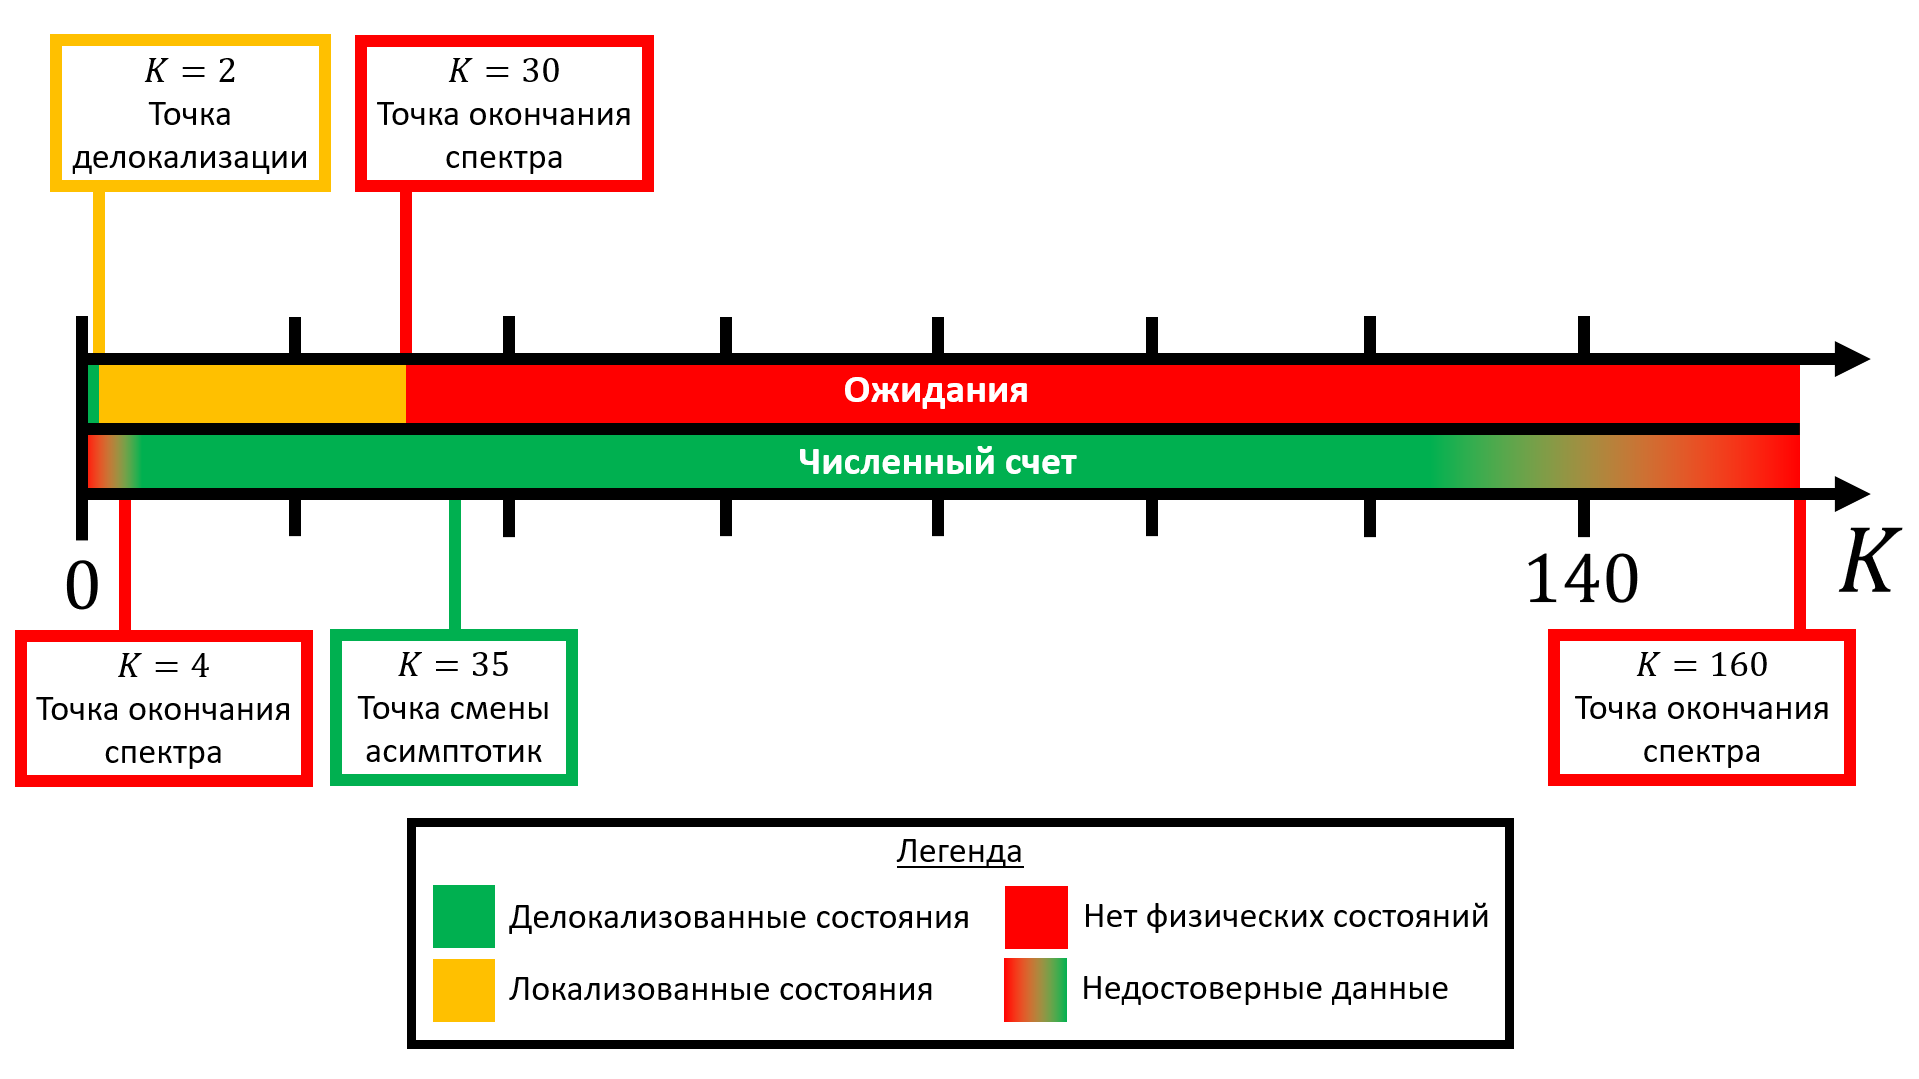
\includegraphics[width=0.9\textwidth]{Phase_diagram.png}
	\caption{Фазовая диаграмма на основании результатов численного счёта. Для сравнения над ней также приведена ожидаемая фазовая диаграмма по статье \cite{FI_microwave}. На диаграмме разным цветом качественно различные диапазоны значений параметров. Градиентной заливкой обозначены неточности в границах зон, вызванные конечной разрешающей способностью численного счёта. На рисунке также отмечены все характерные точки.}
\end{figure}

Чтобы кратко резюмировать качественные сведения, полученные из результатов численного счёта, предлагается фазовая диаграмма, изображённая на Рис. \ref{fig:Phase_diagram}. Для сравнения также приведена диаграмма, предсказанная в \cite{FI_microwave}. Главным выводом, очевидным исходя из этой диаграммы, является то, что эти предсказания \textit{совершенно не подтвердились}. Далее мы разберёмся в причинах этих расхождений.


\section{Основные выводы из результатов}
Подведём итоги увиденного в данных численного счёта: попробуем объяснить расхождения с теоретическими предсказаниями и дадим интерпретацию результата в терминах исходной задачи поиска низкоэнергетических возбуждений.


\subsection{Взгляд с точки зрения задачи Андерсона}
Прежде всего, дадим теоретические пояснения различий между реальной картиной и предсказаниями статья \cite{FI_microwave}. Объяснение можно извлечь из ранее упомянутого в \autoref{Numer} совпадения уравнений популяционной динамики \eqref{eq:Population_dynamics_final_equations} c таковыми для задачи локализации Андерсона на решётке Бете с диагональным беспорядком $\frac{K}{g} \eta^{-1}$ на узле в центре зоны (далее, просто <<задачи Андерсона>>). Авторами статьи \cite{FI_microwave} также неявно было использовано это соответствие, но только в приближённой редакции т. н. Anderson's Upper Limit Condition \cite{AAT}, что и приводит к расхождения с численными данными. Более детальные рассуждения следующие:
\begin{itemize}
	\item Положение точки локализации $K_1$ в работе \cite{FI_microwave} находилось из следующего условия, эквивалентного оценке Anderson's Upper Limit:
	\begin{eqnarray}
		\label{eq:IF_condition}
		\exp \left\{ f(x) \right\} \equiv K \int \limits_0^1 d\xi \left[ \frac{g}{K} \eta\left(\omega|\xi\right)^{-1} \right]^{2 x}= 1, \frac{\partial f}{\partial x} = 0
	\end{eqnarray}
	С точки зрения буквально задачи Андерсона, решение этого уравнения эквивалентно наличию распределения плотности состояний со степенным поведением с показателем $x + 1$. Приближение же состоит в том, что при выводе происходит пренебрежении статистикой действительной части функции Грина. Однако, более аккуратный анализ точного интегрального уравнения, возникающего на распределение плотности, позволяет показать \cite{AAT}, что строго в точке перехода величина $x$ \textit{всегда равна критическому значению $x_c = 1/2$}. С учётом этой поправки, уравнение даёт правильный ответ в лидирующем порядке по $1/K$. Однако, с этой точностью при подстановке правильного значения $x = 1/2$ сам параметр $K$ \textit{из уравнения полностью исчезает}, что означает отсутствие какого-либо перехода по параметру $K$ c точностью $1/K$. Заметим, что описанная согласно \cite{AAT} картина полностью подтверждается численным счётом, в том числе количественно:
	\begin{itemize}
		\item состояния делокализованы при всех $K$, при которых они вообще наблюдаются.  
		\item Однако, если подставить в уравнение \eqref{eq:IF_condition} правильное значение $x = 1/2$, то при $\omega = 0$ мы получим \textit{буквально уравнение самосогласования теории БКШ \eqref{eq:Order_parameter_self_consitency_BCS_limit}}, которое в нашей модели всегда выполнено. Следовательно, наша модель \textit{всегда} находится близко к порогу локализации. Это прекрасно согласуется с наблюдаемой картиной: мы всегда наблюдаем критическое значение показателя степени у распределения плотности состояний и значительное отличие между средним и типичным.
		\item В связи с этим фактом также существует вероятность, что в областях, которые не удалось разрешить численным счётом, состояния локализуются перед тем, как исчезнуть. Это предположение не лишено смысла, так как при ненулевом беспорядке в стандартной задаче Андерсона на дереве между краем спектра и точкой локализации есть область конечного размера по энергии с локализованными состояниями \cite{Biroli_2010}.
	\end{itemize}
	\item Значение точки исчезновения состояний $K_2$ ранее находилось с помощью того же приближенного уравнения \eqref{eq:IF_condition} в предположении, что состояния локализованы перед тем, как пропадут. Однако, как мы убедились, эти предпосылки изначально неверны, а потому положение края спектра для данной модели также найдено неверно. 
\end{itemize}

Развитая на данный момент теория задачи Андерсона позволяет сделать ещё ряд качественных и количественных заключений, важных для понимания полученных результатов. Далее мы будем активно опираться на статью \cite{Biroli_2010}.
\begin{itemize}	
	\item \textit{С математической строгостью} можно найти точное значение края непрерывного спектра (того, что даёт конечный вклад в плотность состояний в термодинамическом пределе). Далее мы приведём рассуждения физического уровня строгости, которые могут быть аккуратно доказаны. Край спектра задачи Андерсона определяется исключительно случаями <<резонансного>> поведения беспорядка, когда в образце образуется большая область с одинаковым значением случайных величин, задающих беспорядок. Такой области соответствует значение энергии
	\begin{equation}
		\label{eq:Edge_energy_Anderson_model}
		E_* = 2 \sqrt{K} - \frac{K}{g} \frac{1}{\eta_{min}} = 2 \sqrt{K} - \frac{\Delta K}{g}
	\end{equation}
	где первое слагаемое -- максимальное собственно значение непрерывного спектра оператора Лапласа на решётке Бете, а второе слагаемое -- максимальное значение беспорядка. Нас интересует собственное число $E = 0$, а потому край спектра определяется условием $E_* = 0$, откуда получаем:
	\begin{equation}
		\label{eq:Edge_of_the_spectrum_in_Anderson_model}
		K_* = \left( \frac{2 g}{\Delta} \right)^2 = g^2 \exp\left\{ \frac{2}{g} \right\}
	\end{equation}
	\item Однако, при использованных в численных симуляциях значениях $g$ край спектра находится в точке $K_* \approx 1.4 \cdot 10^4$. Возникает резонный вопрос: почему же полученная нами оценка на положение края спектра $K \sim 160$ даже по порядку величины неверна? На сей раз, строгого ответа у автора данной работы не имеется, но возможно дать убедительное полуколичественное рассуждение: как уже упоминалось, край спектра находится в точке \eqref{eq:Edge_of_the_spectrum_in_Anderson_model} за счёт областей, в которых величины беспорядка все приняли близкие значения. Вклад в плотность состояний, соответствующую таким областям, можно оценить на основе вероятности такого совпадения значений. Следуя методике, предложенной в \cite{Biroli_2010}, для нашей системы получаем, что зависимости плотности состояний от расстояния до края спектра по энергии $\delta E$ есть
	\begin{equation}
		\label{eq:DoS_near_edge_estimation}
		\rho(\delta E) \sim \exp \left\{ -\frac{K+1}{K} K^{\pi K^{1/4} / \delta E^{1/2} } \ln \frac{1}{ \sqrt{2 \Delta \delta E} } \right\}
	\end{equation}
	Далее, поскольку в терминах задачи Андерсона мы интересуемся плотностью состояний на энергии $E = 0$, то $\delta E \equiv E_*$ -- некоторая плавная функция $K$. С другой стороны, функция \eqref{eq:DoS_near_edge_estimation} является \textit{очень резкой}, так что при приближении к краю спектра эта плотность состояний очень быстро принимает микроскопические значения. На практике полученная величина \eqref{eq:DoS_near_edge_estimation} является оценкой снизу, в то время как реальная плотность состояний обеспечивается и другими механизмами кроме вышеописанной схемы <<резонансов>>. Поэтому в момент, когда все прочие механизмы теряют свою эффективность, плотность состояний практически мгновенно принимает значения, не отличимые от нуля никакими практическими методами, в том числе и численными. Именно этот факт и отражает найденная нами точка $K \sim 160$.
	\item Наконец, ещё одно важное следствие приведённых рассуждений состоит в том, если описанное поведение в духе уравнения \eqref{eq:DoS_near_edge_estimation} действительно имеет место, то край спектра задачи \textit{не имеет никакого физического значения}: если им задаётся какая-то реальная физика, то столь малая плотность состояний не обнаружима никакими доступными экспериментальными методами.
\end{itemize}


\subsection{Интерпретация в терминах исходной задачи низкоэнергетических возбуждений}
Наконец, дадим некоторые комментарии по поводу значения полученных результатов для исходной задачи описания низкоэнергетических возбуждений в сверхпроводнике. Изначально она ставилась в терминах спектральных свойств некоторого, вообще говоря, нелокального оператора \eqref{eq:Investigated_linear_operator}, после чего было показано, что конечная плотность состояний и свойства локализации собственных мод в этой задаче связаны некоторой гладкой ненулевой функцией с таковыми для локального оператора \eqref{eq:Local_operator_definition} в собственном значении $1$. На основании этих рассуждений и полученных нами результатов можно сделать главные на данный момент выводы по проделанной работе: 
\begin{itemize}
	\item поскольку плотность состояний локального оператора вблизи края спектра ведёт себя негладки образом, то такого же неаналитического поведения следует ожидать и от плотности возбуждений. А значит, и для исходного оператора \eqref{eq:Investigated_linear_operator} вопрос края спектра также не имеет глубокого смысла, поскольку такая ничтожная плотность состояний не может быть обнаружена никакими физическими опытами.
	\item Поскольку свойства локализации у двух задач совпадают, а для локальной задачи наши результаты состоят в том, что моды всё время делокализованы, то тоже самое верно и для возбуждений в рамках изучаемой модели. В частности, результаты потенциально означают диссипативное поведение во всей области параметров, что уже прямо противоречит экспериментальной картине.
\end{itemize}
Резюмируя, \textit{построенная модель не отображает реальной физики низкоэнергетических возбуждений}. Укажем несколько возможных причин и следующие из них пути улучшения построенной модели.
\begin{itemize}	
	\item Главной причиной автор работы считает приближение, связанное с игнорированием распределения параметра порядка по узлам системы. Как мы видели в обсуждении полученных зависимостей, локализация в данной задаче не наступает с точностью $1/K$. Единственным эффектом порядка $1/K$, который был выкинут при построении модели, являются отклонения параметра порядка от своего среднеполевого значения \eqref{eq:Order_parameter_BCS_limit}. Напомним также, что это приближении лишает локальный оператор \eqref{eq:Local_operator_definition} собственного состояния с собственным числом $1$, являющегося Голдстоуновским возбуждением нарушенной фазовой $U(1)$-симметрии. 
	
	\item Далее, важно упомянуть, что строго говоря, в \autoref{Theor} был установлен лишь факт совпадения положения характерных точек обеих моделей. При этом никаких утверждений касательно количественной связи плотности состояний в двух моделях не делалось. Поэтому в общем случае необходимо также исследовать, как связаны количественные характеристики двух моделей.ы
\end{itemize}


\subsection{Планы дальнейших исследований}
Как следует из обсуждения выше, дальнейшее направление развития построенной модели следующее:
\begin{itemize}
	\item изучить более подробно решение уравнения самосогласования \eqref{eq:Order_paramter_self_consistency} в следующем порядке по $1/K$ и, в частности, исследовать возникающее совокупное распределение полей $\eta_i$, в которые входит значение параметра порядка на узле, тем самым делая величины $\eta_i$ также коррелированными.
	
	\item По итогам исследования структуры решения уравнения самосогласования необходимо поставить задачу, учитывающую найденные корреляции и пригодную для численного и/или аналитического исследования.
	
	\item С другой стороны, вполне вероятно, потребуется модификация существующей численной процедуры, учитывающая корреляции на узлах. В частности, метод популяционной динамики в исходной редакции не приспособлен к исследованию коррелированного беспорядка.
	
	\item Отдельным пунктом можно упомянуть исследования степени количественной схожести спектральных задач для операторов \eqref{eq:Investigated_linear_operator} и учитывающего корреляции варианта оператора \eqref{eq:Local_operator_definition}, так как на данный момент продемонстрирована лишь соответствие их качественного поведения.
\end{itemize}

\chapter{Заключение} \label{Concl}
В данной работе рассмотрена общая теория описания микроскопически неоднородных сверхпроводников вблизи перехода <<сверхпроводник-изолятор>>, и на основе представленного формализма приведён подход к описанию низкоэнергетических коллективных возбуждений в рассматриваемом классе систем.

Мотивацией исследования выступили многочисленные экспериментальные данные оптической спектроскопии, свидетельствующие о наличии в грязных сверхпроводниках коллективных возбуждений с энергией меньше ширины сверхпроводящей щели.

В \autoref{Theor} работы приводится подробный обзор уже имеющихся феноменологических, экспериментальных и теоретических сведений, существенных для построения общей модели сверхпроводников вблизи перехода <<сверхпроводник-изолятор>>. Далее на основе развитого формализма строится желаемая модель низкоэнергетических возбуждений и обсуждаются аспекты её применимости. 
\begin{itemize}
	\item Роль центрального объекта в этом описании играет псевдоспиновый гамильтониан \eqref{eq:Ham_final}, описывающий многочастичную квантовую механику преформированных электронных пар. В соответствующей части приводится полная феноменологическая база, приводящая к данной модели. Ключевыми феноменами, позволяющими рассматривать задачу таки образом, являются комбинация эффектов локализации одночастичных состояний за счёт сильного беспорядка и феномен преформирования электронных пар, сводящий динамику системы в релевантном диапазоне энергий к туннелированию электронных пар. Формулировка модели также требует принять ряд чисто качественных упрощений, призванных максимально упростить вызванную эффектами локализации сложную структуру одночастичных состояний и их перекрытий.
	\item С помощью семионного представления Попова-Федотова и методов функционального интегрирования приводится вывод основных уравнений сверхпроводимости --- уравнения самосогласования \eqref{eq:Order_paramter_self_consistency} и оператора, определяющего квадратичную часть функционала Гинзбурга-Ландау \eqref{eq:Order_parameter_fluctuation_inverse_propagator_explicit}. Существенным плюсом используемого подхода является имеющаяся возможность последовательно выяснять границы применимости стандартного среднеполевого формализма на основе нескольких вариантов диаграммной техники.
	\item В терминах квадратичной части функционала Гинзбурга-Ландау сформулирована задача, описывающая низкоэнергетические возбуждения в рассматриваемой системе.
	\item Сделано ключевое предположение о нерелевантности отклонения распределения параметра порядка от своего среднеполевого предела, которое позволяет свести задачу к изучению устройства спектра локального оператора \eqref{eq:Local_operator_definition}. Существенным является то, что использованное приближение лишает систему возбуждения Голдстоуна, являющегося следствием нарушения $U(1)$-симметрии.
\end{itemize}

В \autoref{Numer} описывается численный метод популяционной динамики, пригодный для изучения широкого класса задач локализации. 
\begin{itemize}
	\item Описаны теоретические аспекты устройства больших $K$-регулярных графов, связывающие их локальные свойства со свойствами этих величин на решётке Бете.
	\item В терминах производящего функционала представлен вывод метода популяционной динамики. Установлено, что данный метод является эквивалентном замкнутого интегрального уравнения на распределение диагональных элементов функции Грина линейного оператора на графе.
	\item Обсуждён правильный предельный переход для исследования спектральных характеристик именно задачи на $K$-регулярном графе. Порядок пределов определяется отсутствием у регулярного графа границы и вытекающими из этого условиями самосогласования.
	\item Продемонстрировано, что исследуемая задача благодаря конкретной структуре беспорядка в рамках используемых приближений эквивалентна хорошо изученной задаче локализации Андерсона.
	\item В работе также подробно обсуждены особенности поведения алгоритма популяционной динамики применительно к конкретной задаче. В частности, отмечено влияние внутренних параметров алгоритма, определяющее границы численной применимости всего метода.
\end{itemize}

Наконец, в \autoref{Result} приведена сводка полученных результатов численного исследования задачи, приведено подробное обсуждение этих результатов и намечен план дальнейших исследований.
\begin{itemize}
	\item В рамках проведённого исследования модель демонстрирует наличие делокализованных возбуждений во всём диапазоне параметров. Существенно, что этот факт расходится с утверждениями в работе \cite{FI_microwave}, предсказывавшими существования точки локализации состояний. Расхождения объясняются с привлечением задачи Андерсона, а именно, некорректно использованным приближением Anderson's Upper Limit. 
	\item Полученное распределение плотности состояний демонстрирует степенной хвост в широких пределах с характерных показателем степени $3/2$. Данное поведение приводит также к отличию средней и типичной плотности на три порядка. Результат находится в полном согласии с теории локализации Андерсона, так как при указанном выборе параметров модель всё время находится вблизи точки перехода c делокализованной стороны.
	\item Изучены зависимости характеристик распределения от числа ветвления графа $K$, на основании результатов построена фазовая диаграмма на Рис. \ref{fig:Phase_diagram}. Основными особенностями является видимое исчезновение состояний при очень малых $K \le 6$ и очень больших $K \gtrsim 160$ значениях параметра, а также явно присутствие точки смены асимптотик $K = 35$, степень физической значимости которой осталось невыясненной. Поведение модели на больших $K$ снова расходится с предсказаниями статьи \cite{FI_microwave}. Причиной расхождений является уже упомянутое приближение Anderson's Upper Limit, привёдшее к неверному предположению об устройстве состояний перед исчезновением.
	\item Проведена математически строгая оценка точного положения края спектра для данной задачи. Однако, численно значение оказывается на два порядка полученного численными методами. Расхождение объясняется конечной разрешающей способностью и метода и, что более важно, очень резким неаналитическим убыванием плотности состояний при приближении к краю спектра.
	\item В терминах исходной задачи низкоэнергетических возбуждений полученные результаты означают несостоятельность изучаемой модели, а значит, сделанных при её получении допущений. Ключевым предположением, приводящим к несостоятельным результатам, признано пренебрежение распределением и корреляциями параметра порядка на различных узлах.
	\item На основе полученных данных построены дальнейшие планы исследований. Основным направлением деятельности выделяется более тщательное изучения устройства распределения параметра порядка и связанные с этим модификации модели.
\end{itemize}

Автор данной работы выражает искреннюю благодарность своим научным руководителям Михаилу Викторовичу Фейгельману за многочисленные и в высшей степени информативные обсуждения данной задачи и Константину Сергеевичу Тихонову за неоценимую помощь в освоении всех технических аспектов теоретической и численной части данного исследования.

% список литературы
\bibliographystyle{unsrt}
\bibliography{Thesis_bibliography}

% Приложения
%\begin{appendices}
	\chapter{Семионное представление конечномерной алгебры Ли} \label{App_Semion}
	\section{Гомоморфизм представлений}
	\section{Вопроизведение статсуммы}
\end{appendices}

\end{document}